\documentclass[twocolumn]{article}
\usepackage{preprint}

\usepackage[utf8]{inputenc}
\usepackage[T1]{fontenc}
\usepackage{amsmath}
\usepackage{amssymb}
\usepackage{graphicx}
\usepackage{array}
\usepackage{booktabs}
\usepackage{multicol}
\usepackage{longtable}
\usepackage{xcolor}
\usepackage[colorlinks=true,linkcolor=cyan,urlcolor=blue,citecolor=cyan,anchorcolor=black]{hyperref}
\urlstyle{same}
\makeatletter
\g@addto@macro\UrlBreaks{\do\-\do\a\do\b\do\c\do\d\do\e\do\f\do\g\do\h\do\i\do\j\do\k\do\l\do\m\do\n\do\o\do\p\do\q\do\r\do\s\do\t\do\u\do\v\do\w\do\x\do\y\do\z\do\A\do\B\do\C\do\D\do\E\do\F\do\G\do\H\do\I\do\J\do\K\do\L\do\M\do\N\do\O\do\P\do\Q\do\R\do\S\do\T\do\U\do\V\do\W\do\X\do\Y\do\Z\do\0\do\1\do\2\do\3\do\4\do\5\do\6\do\7\do\8\do\9}
\makeatother
\hypersetup{pdftitle={Long-Horizon AI-Augmented Engineering under Complexity}}
\usepackage[numbers,square]{natbib}
\bibliographystyle{unsrtnat}
\usepackage{authblk}
\makeatletter
\renewcommand\AB@authnote[1]{}
\renewcommand\AB@affilnote[1]{}
\makeatother
\renewcommand\Affilfont{\footnotesize}

\setlength{\leftmargini}{0.5\leftmargini}
\setlength{\leftmarginii}{0.5\leftmarginii}
\setlength{\leftmarginiii}{0.5\leftmarginiii}
\setlength{\leftmarginiv}{0.5\leftmarginiv}
\setlength{\leftmarginv}{0.5\leftmarginv}
\setlength{\leftmarginvi}{0.5\leftmarginvi}

\makeatletter
\def\@halvelistgap{\topsep0.5\topsep \partopsep0.5\partopsep}
\g@addto@macro\@listI{\@halvelistgap}
\g@addto@macro\small{\g@addto@macro\@listi{\@halvelistgap}}
\g@addto@macro\footnotesize{\g@addto@macro\@listi{\@halvelistgap}}
\makeatother

\title{Long-Horizon AI-Augmented Engineering\\under Complexity\\[0.08in]{\large\normalfont\itshape An Inquiry into Principles and a Framework for Keeping Complex Work Coherent Across Time}}
\author[1]{Franz Bruckhoff}
\affil[1]{\href{https://stratington.com}{stratington.com} \textbar{} \href{https://think-bigger.org}{think-bigger.org}}
\day=25 \month=9 \year=2026

\begin{document}

\lhead{\scshape Preprint \textperiodcentered{} Long-Horizon AI-Augmented Engineering under Complexity \textperiodcentered{} Franz Bruckhoff}

\twocolumn[
  \begin{@twocolumnfalse}
  \maketitle
  \begin{abstract}
  \begin{multicols}{2}
  Until recently, the development of highly complex engineered systems was usually reserved for large organizations. What those organizations supplied was not only labor, but the structure that held their work together across many years. The emergence of powerful agentic AI has redefined the scale of what one person, or a small team of two to three, can realistically attempt and accomplish.

  However, complex work over long horizons depends on explicit structure, including bounded components, contracts, verification, and human authority that survive the intervals between decisions and their consequences.

  This paper develops the Framework for Keeping Complex Work Coherent Across Time from mechanisms found in recorded engineering practice.
  Its domain-general core comprises five principles and the separately issued Specification, whose 106 clauses state the structure needed to preserve coherence and name their grounds in a generalized pattern, a principle, or a stated goal.

  The paper reprints the principles and the clauses in an appendix.
  It gives the reasoning behind them, explains their derivation, and analyzes the resulting artifacts for internal coherence and traceability.

  A semantic graph represents the clauses, their grounds, their terms, and their relations to stated goals.
  It supports static analysis of the framework's internal coherence. An internal rebuild from fixed inputs and recorded decisions matched the recorded relation graph exactly.

  The problem is the coherence of a complex project across years: whether its purpose, its contracts, its authority, and its terms of acceptance still hold when most of the work is carried out by AI agents under human direction.
  Stronger execution at each step does not produce that coherence.
  The framework makes the structure once supplied by large organizations explicit and durable for one person or a small team working with AI agents.
  \end{multicols}
  \end{abstract}
  {\footnotesize\centering\textcopyright\ 2026 Franz Bruckhoff. This work is licensed under a Creative Commons Attribution-ShareAlike 4.0 International License (CC BY-SA 4.0):\newline\url{https://creativecommons.org/licenses/by-sa/4.0/}\par}
  \vspace{0.35cm}
  \end{@twocolumnfalse}
]

\section{Introduction}

\subsection{Problem and scope}

As of September 2026, long-horizon AI-assisted engineering without adequate supporting structure and methodology is vulnerable to gradual loss of coherence. Such degradation can be difficult to detect early.

While individual tasks may complete correctly, the relationships binding them eventually erode in various ways: They become incorrect, inconsistent, ambiguous, stale, detached or are lost entirely.

For example, a contract might be misread, causing the implementation of an interface against a behavior that was never authorized by the specification. Multiple specifications might state different acceptance criteria targeting the same system behavior with unclear prioritization. Stale requirements might keep interfering long after the underlying decisions have been reversed. Stale tests may keep passing while the criteria to be verified had been changed quietly.

This decay accelerates, and one reason for this is that AI agents operate without institutional memory. While humans absorb unwritten history and implicit consensus into tacit knowledge, AI agents presently only evaluate the bounded context provided to them at execution time.

Each isolated session produces locally optimal work that can remain completely oblivious to the project's accumulated decisions, the grounds and authority behind them, and the cross-cutting commitments made weeks, months or years earlier. As people turn over and tooling evolves, this lack of institutional machine-accessible memory compounds into drift that is effectively irreversible.

To resolve these problems, it is necessary to externalize transient conversational instructions and tacit human knowledge into durable, machine-readable structure, contracts, methods, and records. The key to keeping long-horizon systems coherent across time is to anchor the project's governing invariants and contracts through human authority in a machine-readable way, while automated verification continuously checks that local changes remain consistent with those explicit constraints and do not silently undermine the project's global intent.

There are six primary classes of failure that can break the relationships underpinning complex, long-horizon projects: late feedback, design obsolescence, loss of purpose, contract loss, loss of evidence, and loss of authority.

When feedback arrives late, wrong decisions may be repeated before their result becomes visible.

When the implementation changes, knowledge bound to the old design is lost silently while the requirement it served may remain in force without anything left to explain it.

When the purpose behind a requirement is forgotten and nothing in the project can explain why it exists, later work may treat it as arbitrary and delete it as unnecessary.

When a contract between two system components is lost from the context of the work that modifies these components, changing one component can break the other in a way that goes unnoticed by either.

When the evidence for an earlier acceptance is lost, later work may be unable to correctly infer which checks justified that acceptance, and may end up verifying against different criteria than the ones originally used, thereby silently drifting the definition of done without anyone deciding that it should.

When the record of who may have authority to approve a change is lost, an AI agent may approve it without a recorded decision, or the change may be pending indefinitely because it is unclear who holds approval authority.

All of these failures tend to go unnoticed, allowing potentially catastrophic systemic errors to propagate long before anyone detects them.

Each occurrence erodes the ability of the humans and AI agents working on the project to detect a mistake before it is repeated, reconstruct the project's prior decisions, understand why the current design and its requirements exist, anticipate what a change will break, reconstruct what had been verified against what, verify present work, or establish who may authorize the next change. These blind spots allow localized mistakes to compound silently into systemic failure that is hard to resolve.

The six classes of failure discussed in this paper are structural, domain-general, and not unique to software. They generally tend to recur in every domain where complex long-horizon work is being done.

Across all kinds of these domains, the essence of these classes of failures stays constant while the conditions under which they occur may vary.

In the software domain, iteration tends to be cheaper in time and effort than in the hardware domain. Verification is relatively fast, and a change to a software component can usually be reversed more easily than a change to a physical one. The difference across domains is the degree to which iteration is cheap, verification is fast, and changes are reversible. The domain sets the default, while detection speed and reversal cost set the outcome.

To illustrate, imagine a coordination platform for autonomous wildfire-response drones, built and operated over the course of many years by a small team of two, with AI agents carrying out most if not all of the heavy implementation work. In year one, the founders commit to the regional fire authority. Their platform retains decision provenance for five years, such that every decision their platform makes during an incident can be fully reconstructed from raw telemetry.

That commitment requires that raw telemetry is safely stored for five years. The replay tool must deterministically reconstruct any intervention from that telemetry, while any change in telemetry format or operating procedure over time keeps old records replayable. Everything is fine until one day three routine tasks touch those areas. One deletes raw telemetry older than six months and keeps only summaries immediately available. Another task rewrites the replay system to run from those summaries. And finally, a task is executed which migrates the telemetry format but converts only live data, leaving the archived data incompatible. Each task passes its tests, while the commitment has been broken three times because it belongs to no single component. The decision behind it sits in a Decision Record from 2025, and no task in 2029 gains awareness of it. One day, the authority investigates a fatal crash of one of the firefighting drones. As it turns out, it is not possible to reconstruct the platform's decisions from eight months before, because the raw telemetry data was deleted and only summaries were kept.

None of the contracts for telemetry data storage, replay, and format stated the commitment to the regional fire authority: The requirement to retain five years of raw telemetry data, deterministic replay under any circumstance, and compatibility across format and operating procedure changes. No contract required the three changes to keep the commitment, therefore they broke no contract.

The solution is to state the commitment in each of the contracts for telemetry data storage, replay and data format, so that any later change to any of them meets it.

In the separately issued framework, such a commitment is a contract under the principle Specifications as Contracts \citep{tbf2026}. A contract here fixes the behavior and acceptance conditions that humans have approved for other components to rely on \citep[Section~\hyperlink{nss-2}{2}]{pss2026}.

But simply restating the commitment in three contracts is not enough. The commitment needs one authoritative source, and the contracts that must uphold it need to point back to that source. Otherwise each contract carries a copy of the commitment, and copies drift.

The commitment to the regional fire authority belongs at the System level. It is one commitment, owned by one named human, and it is the source that the telemetry data storage, replay, and format contracts all serve. Each of those contracts then carries the specific obligation it must preserve. The storage contract carries five-year retention of raw telemetry. The replay contract carries deterministic reconstruction of any retained incident. The format contract carries continued replayability of old records across format and procedure changes. Each of those contracts points back to the same top-level commitment, so none of them can be satisfied locally while the commitment is broken globally.

Under Verification-First Engineering, the commitment must be checkable before any of the three changes begin. An independent verifier takes a past incident, replays it from stored raw telemetry, and records whether the reconstruction is deterministic and complete. After a format or operating procedure change, the same check must show that old records still replay. If the check fails, the change is not done. The six-month deletion cannot pass as a storage detail, because the check is against the recorded commitment, not against the local tests of the storage component. The same holds for the replay rewrite and the format migration.

This is what the framework for keeping complex work coherent across time requires of every commitment: a durable record of the purpose it serves, and relations that let a proposed change be traced to everything it can affect.

In the fire-authority example, the storage, replay, and format contracts would each point back to the commitment and the verification that checks it. A proposed change would point forward to every contract, check, and record it can affect.

A task that deletes raw telemetry data after six months would point forward to the storage contract, the fire-authority commitment, and the replay check that depends on the retained data. The AI agent would see that the deletion weakens a commitment it is not authorized to change, and the change would stop before it is accepted. The same would happen for the replay rewrite and the format migration. None of the three could pass on its own tests alone, because its own tests were never written against the commitment it was about to break.

The commitment to the fire authority is then a single commitment, not three. It has one named human owner, and every contract that must uphold it can reach it.

Human authority applies across all five principles. In the example, a change may compress telemetry, change how it is stored, or migrate its format within the recorded commitment. Only the responsible human may shorten the five-year retention period or approve replay from summaries, because those changes weaken a commitment made to the fire authority \citep[Sections~\hyperlink{nss-1.3}{1.3} and~\hyperlink{nss-15.2}{15.2}]{pss2026}. Passing the tests of a single task does not authorize a change to a commitment those tests never checked.

I use two requirements to examine these commitments.

The first is \emph{standing grounds}: each requirement has a durable record of the purpose or prior commitment it serves, with relations that can be followed in both directions. For the platform, the retention requirement would carry the fire-authority commitment it serves, and that commitment would name every requirement that rests on it.

The second is \emph{traversable consequence}: recorded relations let a check find the commitments, records, and tests that need review before a proposed change. For the six-month deletion, those relations would lead from telemetry storage to the fire-authority commitment, its replay check, and the format contract that relies on it.

The five principles organize the work; these two requirements concern the grounds of its commitments and the consequences of changing them.

The same coordination question arises when a physical system changes: which requirements must still hold after a part is replaced, and what evidence will establish that they hold? The form of the evidence differs; the requirement that work is incomplete until verified does not. A software component test and a physical inspection produce different Verification Artifacts. Rules shared across domains must preserve that difference while keeping purpose, interfaces, verification, and authority explicit. The framework places those relations in five domain-general principles, and domain practice supplies the methods used to check a particular system \citep{tbf2026}.

\subsection{Questions and contributions}

Existing engineering practice provides mechanisms for keeping these commitments available: component boundaries, specifications, verification records, and controlled changes. The mechanisms examined in this paper come from public engineering material of organizations that build complex systems, ISO and IEEE process standards, and the working practice of leading individual engineers.

A generalized pattern states a mechanism without tying it to one organization or tool.

In their source organizations, the mechanisms are carried by review bodies, process groups, and people who remember why a rule exists. An individual or small team and multiple AI agents have no such carrier around them. For that individual or team, the mechanisms must survive as written rules and records that humans and agents can follow.

The separately issued Specification turns the generalized patterns and the five principles into requirements for project records and their relations \citep{pss2026}.
It separates what a record must contain from the file or format that holds it. An optional software profile illustrates one filesystem layout that a project can adapt.

Two questions follow.

How can mechanisms already used in practice become engineering rules that apply across domains while giving a project specific requirements to follow?

What do the recorded grounds and relations of those rules reveal about missing support, conflicting requirements, and the effects of a proposed change?

The measurements in this paper examine the issued documents.
Whether their rules keep other projects coherent remains a separate empirical question.

The Specification must itself retain the grounds and change relations it requires of projects \citep{goal2026}. A machine-readable copy of its requirements, linked to their source text, records those relations for inspection.

The inspection shows where grounds are recorded, where relations to goals are missing, and which requirements need review together.
Section~\ref{sec:results} reports the findings with the evidence and review decisions that support them.

Three contributions follow.

\begin{itemize}
\item \textbf{Formulation.} Five principles in a separately issued framework, with reasons for each rule, limits on its use, and a division of human and AI authority across all five.
\item \textbf{Artifact.} A separately issued Specification derived from recorded practice, with clause-level grounds and a machine representation linked to the source text.
\item \textbf{Measurement.} Methods and findings that explain how the recorded grounds were checked, where gaps and conflicts were found, and how the recorded relations were used to trace the effects of a change.
\end{itemize}

\section{Background and Related Work}
\label{sec:related}

\subsection{Decomposition and contracts}

A module earns its boundary by the design decision it keeps to itself, and not by the step of processing it performs \citep{parnas1972}. Its interface shows as little of that decision as it can, so a change inside the module stays inside it. The consequences claimed for that criterion are independent work, understandability, and room to change later. Three of the five principles rest on them.

A second line reads the same split as an economic one. A system divides into visible rules that every part obeys and hidden parts that may then vary on their own, and the value of the division is the freedom it leaves for later \citep{baldwinclark2000}.

Contract specification supplies the other half of the boundary: a routine states what its caller must satisfy before the call, what it guarantees in return, and what stays true across its whole life \citep{meyer1992}. What carries is not the checking but the address of a broken promise: an unmet precondition is the caller's defect, and an unmet postcondition is the supplier's.

A component should depend only on components at least as stable as itself \citep{martin2002}. The dependencies themselves can be written as a matrix \citep{steward1981} and measured across real systems, where recurring core and periphery shapes appear \citep{baldwin2014}.

Much of this work assumes a human developer who reads one module, remembers another, and carries the unwritten reasons between them. An AI agent starts a session with only what the project records hand it. The boundary therefore has to bound what the agent may touch, and it has to be recorded where a machine can read it, which is a requirement the prior work had no reason to state.

Contract specification also leaves open who may change a contract, because in its setting the owner of the class does. Where an agent can draft and implement, the Specification answers that question with a recorded authority rather than with code.

\subsection{Systems and requirements engineering}

Life-cycle process standards fix the groups of process an engineering effort must cover: agreement, organizational project-enabling, technical management, and technical \citep{iso15288}. The separately issued Specification adopts those four groups by name at every level of the system \citep{pss2026}.

Scaling such a standard down is established too: one life-cycle standard was built for very small entities rather than assumed to fit them \citep{laporte2008}.

A kernel language describes the practices a working method is assembled from and tracks their state \citep{essenceomg}, and a process metamodel does the same for process content and its compliance points \citep{spem2}.

Traceability separates into the part that runs forward from a written requirement to design, code, and tests, and the part that runs back to the need and the reasoning that produced it. Practitioners report the backward part as the missing one \citep{gotel1994}.


A requirements smell is a cheap static indicator that one sentence may be defective, a vague quantifier or an actor hidden by a passive, and it asks a human to look rather than returning a verdict \citep{femmer2017}.

Goal-oriented requirements engineering attaches requirements to the goals they serve, and the resulting model is examined for goals with nothing to realize them and for the ways a goal can be obstructed \citep{vanlamsweerde2001, horkoff2017}. The goal-path measurement of Section~\ref{sec:results} descends from that analysis.

These standards assume an organization with separate bodies: a board that controls changes, a verification authority independent of the design authority, and professionals whose training fills what the text leaves unsaid. One person, or a team of two or three, has none of those bodies. Independence then has to come from separating the agent that produces a result from the agent that verifies it, and the text has to carry what a trained professional would otherwise infer.

\subsection{Normative text and automated compliance}

Institutional analysis decomposes a written rule into its parts: the actor it binds, the operator that compels or permits, the action, the context in which it applies, and the consequence of breach \citep{crawford1995}. A revised specification, a coding guide, and parser tooling carry that decomposition to scale \citep{frantz2021, frantz2020codebook, frantz2025parser}.

That grammar is the nearest recorded ancestor of the proposition schema used later. Applying it is not free: coding two statutes under it surfaced the reliability problems of hand encoding \citep{basurto2010}.

Norms can travel with their provenance, their temporal scope, and a link back to the passage they were drawn from \citep{legalruleml}, and legal documents have a machine-readable vocabulary for their structure \citep{akomanotoso, palmirani2011}.

A nationality statute was expressed as a logic program in 1986 \citep{sergot1986}, and the principle that a representation should follow the structure of its source, rather than a structure convenient to the tool, was named shortly after \citep{benchcapon1992}.

A recent form binds the two together, with executable semantics written beside the legislative text they implement \citep{catala2021}. Of the located work, that is the closest to the source binding adopted in Section~\ref{sec:checks}.

Most of the field points outward, from the rules to something governed by them. Formalized norms are used to check a business process or an artifact for conformance \citep{governatori2016, hashmi2015}, and a review of compliance checking for software processes reports the same direction throughout \citep{castellanos2022}. Building regulations are turned into structured rules and annotated corpora, and the design is what gets checked \citep{hettiarachchi2025}.

A smaller group points at the normative document itself. Typed relations have been built over a requirements document to make its structure analyzable \citep{grosser2022}. A language specification has been mechanized, and the mechanization surfaced defects in that specification \citep{watt2018}. Statutory text has been encoded with model assistance and then checked deterministically for inconsistency \citep{yadamsuren2026}. A governing catalogue of security controls has a machine-readable form built to support assessment \citep{piez2019}. Table~\ref{tab:relatedwork} sets that group beside the outward-facing one.

In most of this work the text belongs to another body, changes relatively infrequently once issued, and is read by a profession trained to interpret it. The text examined in this paper is the project's own and is under revision, so a proposed edit has to be traced to everything it can affect, which a pipeline checking artifacts against a settled regulation rarely needs.

Model-assisted formalization reports how far it can be trusted: its accuracy holds under guided prompting, direct one-step formalization and fine-tuning produced no measurable gain, and each encoding stays an interpretation whose reference standard may itself be unavailable \citep[Sections~5.1 and~6]{horner2025}. Where the evidence does not settle a question in this paper, no proposition is produced and a classified gap is recorded instead.

\subsection{AI agents and instruction files}

Surveys now organize the use of language models, and of agents built on them, across software engineering tasks \citep{hou2024, liu2024}. These taxonomies do not explicitly address the structure of the project an agent works inside.

Degradation over a long horizon is measured rather than assumed. A study of production decision-making reports task success falling as the number of dependent steps grows \citep{mittal2026}, and a benchmark measures reward hacking in long-horizon coding agents \citep{specbench2026}. Both are preprints, and the first is a single study.

The repository instruction file is the practice closest to the governance documents the Specification requires. It is widespread: one study locates 2,303 agent context files across 1,925 repositories \citep{chatlatanagulchai2025readme}, and an earlier one locates 253 such files over 242 repositories \citep{chatlatanagulchai2025manifests}.

Its measured effect is mixed, and the mixture is the useful part. One study associates the presence of such a file with lower runtime and reduced token use \citep{lulla2026}. An evaluation on real tasks reports no general gain in task success and more than 20 percent higher inference cost \citep{gloaguen2026}.

Two further results find nothing at all. A two-agent ablation on existing repositories reports no measurable effect on correctness \citep{khatri2026}, and a factorial study reports no detectable effect from the file-structure variables it tested, and associates longer sessions with lower adherence \citep{mcmillan2026}.

Priority between instructions has been trained into models \citep{wallace2024} and has been shown to fail even under simple instruction conflicts \citep{geng2025}. A rule an agent is meant to obey is therefore not a control on its own.

These studies measure a single session on a bounded task in a repository that already exists. Whether a project record keeps a multi-year effort coherent is a different question, and none of them answers it.

I do not claim that an instruction file improves the performance of an agent. The adverse results argue for limiting what such a document carries and for routing from it into a versioned structure, which is what the Specification requires of it \citep{pss2026}, and they leave the durable record untested.

\subsection{What is prior art and what is not}

Every mechanism named above is prior art, and I claim none of it as new. Decomposition by hidden decision, interface obligations and invariants, life-cycle process groups, traceability, goal coverage analysis, and standards scaled to small organizations are established practice, as is binding a normative document to a machine-checkable graph. The derivation record names where each one was found.

Three properties stand together in this work, and I claim only their combination as new.

The first is a derivation of a normative document from a mixed and largely practitioner-authored evidence base, with a recorded decision for every candidate at every stage.

The second is one domain-general normative document in which every clause names its grounds, with the completeness of that naming checked by machine in both directions.

The third is the application of that machinery to the governing document itself rather than to an artifact governed by it, under a requirement of an exact source span for every represented unit, an evidence policy that abstains and records a classified gap rather than resolving a disagreement, and a boundary that keeps every finding, traversal, and change calculation free of model calls.

That combination was not found in the searched literature. The search used two working scholarly indexes and the primary records of the publishers and standards bodies involved, so it bounds what was located and not what exists.

\begin{table*}[t]
\centering
\small
\setlength{\tabcolsep}{4pt}
\caption{The traditions this work draws on, the unit each one represents a rule in, the check that unit supports, and the part of this work it grounds. Representative works only; the text names the rest. The last row reports the setting rather than an adopted mechanism.}
\label{tab:relatedwork}
\begin{tabular}{>{\raggedright\arraybackslash}p{1.15in}>{\raggedright\arraybackslash}p{1.35in}>{\raggedright\arraybackslash}p{1.25in}>{\raggedright\arraybackslash}p{1.35in}>{\raggedright\arraybackslash}p{1.40in}}
\toprule
\textbf{Tradition} & \textbf{Representative work} & \textbf{Unit of representation} & \textbf{Check it supports} & \textbf{What it grounds} \\
\midrule
Decomposition and contracts
& \citet{parnas1972}; \citet{meyer1992}; \citet{baldwinclark2000}
& Module, routine, visible design rule
& Interface conformance; precondition and postcondition
& Component-Oriented Decomposition, Layered System Architecture, Integrated Modularity First, Specifications as Contracts \\
\addlinespace
Systems and requirements engineering
& \citet{iso15288}; \citet{gotel1994}; \citet{femmer2017}; \citet{vanlamsweerde2001}
& Process group, requirement, trace link, goal
& Process coverage; traces in both directions; static defect indicators; goal coverage
& The required records, the grounds named by every clause, and the goal-path check \\
\addlinespace
Normative text and automated compliance
& \citet{legalruleml}; \citet{frantz2021}; \citet{catala2021}; \citet{governatori2016}
& Norm with provenance, institutional statement, statute bound to code
& Conformance of a process or artifact to formalized norms
& The proposition schema, the source-bound representation, and the conflict check \\
\addlinespace
Checks on a normative document
& \citet{grosser2022}; \citet{watt2018}; \citet{yadamsuren2026}; \citet{piez2019}
& Requirements document, specification prose, statute, control catalogue
& Structural relations, mechanized semantics, inconsistency detection, assessment support
& Application of the checks to the Specification itself \\
\addlinespace
AI agents and instruction files
& \citet{mittal2026}; \citet{chatlatanagulchai2025readme}; \citet{gloaguen2026}; \citet{wallace2024}
& The session, the repository context file
& Task success, instruction adherence
& The setting, and the limits on what a governance document carries \\
\bottomrule
\end{tabular}
\end{table*}

\section{Construction and Review Method}\label{sec:method}

\subsection{Design and screening}

A source statement is one recorded practice claim taken from one document. A pattern, called an adopted form once generalization accepts it, is a domain-general rule derived from one or more source statements. A clause is a numbered normative sentence of the Specification. The construction runs in that order, and each step keeps the record of the step before it.

The corpus is practice-first. Engineering practice supplies the candidate rules, because the six failure classes appear in project records long before they appear in papers. The literature enters later, and only to name mechanisms and to bound claims.

Five collection rounds produced 219 source statements. Each round dispatched isolated collectors, twenty in total, and each collector recorded what its assigned sources stated without judging the statement. Filtering was forbidden at this step, so that a later gate could act on a stable population. The orchestrator did not independently refetch every source, so a recording error by a collector survives into the screened population.

Screening then read each of the 219 candidates in isolation. One classifier saw one candidate and one fixed decision block, and saw no other candidate and no running tally. The block asked five questions. Four are hard gates: the statement must generalize beyond its own domain, must strengthen decomposition, contracts, or verification, must preserve human authority over purpose, invariants, risk acceptance, and the definition of done, and must reduce rather than multiply mechanisms. The fifth question assigns a stability class and rejects nothing. Every answer was recorded verbatim, and no answer was later overridden.

The screen kept 113 statements and rejected 106. Of the kept statements, 110 are stable and 3 are volatile. Five rejected statements were then readmitted by a separate and narrower rule: the recorded rejection reason had to name domain specificity as the primary failure, and the statement had to carry a transferable idea that the kept set did not already hold. Each readmission carries its written justification. The two populations stay distinct: 113 statements passed the screen, and 118 statements entered generalization. Figure~\ref{fig:funnel} carries the whole flow.

\begin{figure*}[t]
\centering
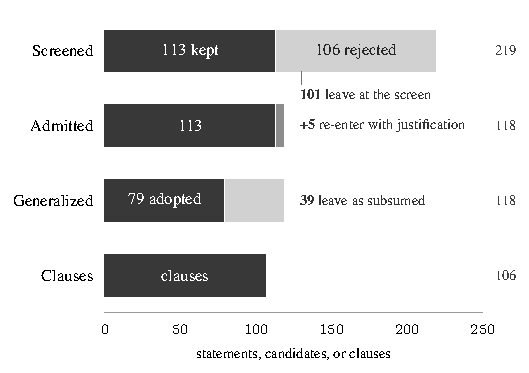
\includegraphics[width=\textwidth]{figures/f01/f01-funnel.pdf}
\caption{The construction funnel. Collection produced 219 source statements. The isolated screen kept 113 and rejected 106. Five rejected statements were readmitted under the secondary rule, giving 118 inputs to generalization. Generalization adopted 79 forms and discarded 39 as subsumed, with none parked. The adopted forms were expressed as 106 numbered clauses; the last row counts clauses, not candidates.}
\label{fig:funnel}
\end{figure*}

The design follows the design-science cycle of \citet{peffers2007}, which builds an artifact against a stated problem and then evaluates it, and it treats practice documents as admissible evidence in the manner of the multivocal review \citep{garousi2019}. The reporting follows the empirical-standards guidance for design-science and methodological work \citep{ralph2021,baltes2026}, and the construction of a method from named, reusable fragments follows method engineering \citep{brinkkemper1996}. Three departures from those frames are recorded. The protocol was not registered before collection. The screening decisions received no independent human validation, and the correction and review passes described below are the substitute. I stopped collection when I judged that the sources supplied no further mechanisms, not when a measured coverage threshold was met.

\subsection{Generalization and correction}

I established the vocabulary used to generalize the 118 candidates in one pass. Isolating each candidate, as the screen did, would have been the consistent choice, and it fails here for a structural reason: the risks of this step are dilution and duplicate mechanisms, and neither is visible from one candidate. The vocabulary was fixed before the first restatement, and software-specific nouns were excluded from every restatement.

Each candidate received the same five-part record: the original form, an abstract mechanism stated without domain-specific nouns, a domain-general restatement, an explicit answer to three tests, and one decision of adopt, discard, or park. The three tests repeat the three substantive gates of the screen, now applied to the restatement rather than to the source: it must still strengthen decomposition, contracts, or verification, must still preserve human authority, and must still reduce rather than multiply mechanisms.

Duplicates were resolved by subsumption rather than by deletion. Where several candidates carried one mechanism, one restatement was adopted as the canonical form, and every other candidate was discarded with an explicit pointer to the form that absorbed it. Distinct facets of a discarded candidate were folded into the canonical restatement when they added force. Decision records show the shape: \hyperlink{gp-60}{GP-60} is the adopted form, six candidates are discarded as subsumed by it alone, and a seventh names it among the forms that absorb it. A discard at this step never reopens the screening decision; it states only that the candidate is not a separate clause.

The pass adopted 79 forms, grouped into 12 mechanism families, discarded 39 as subsumed, and parked none. No candidate carried value that applied to software alone.

Verification then ran as a separate pass with a different model, against 101 distinct source pages. It applied six criteria and two mechanical checks, and it reported findings without editing the file it checked. The pass recorded 58 forms as correct and 21 as needing revision, and failed none. Revision was therefore needed for 21 of the 79 adopted forms at first writing. This observed first-pass defect rate characterizes this execution of the method and should not be interpreted as an estimate of the method's general error rate.

Correction ran after verification and was bound to its findings. All 21 forms were revised. The fixed terminology block grew from 13 to 21 terms, because load-bearing terms had no definition and the relation between specification and contract was not used consistently. Four conflicts between adopted forms were resolved by narrowing exactly one form of each pair, so that no pair was left mutually exclusive. A third model then ran the final check and confirmed that all 21 corrections were present in the file.

Expression as clauses followed. The adopted forms were rewritten as numbered normative sentences with their actor, modality, and object made explicit, which produced the 106 clauses of the Specification. A clause may carry more than one form, and each clause names the forms it carries in its grounds. Section~\ref{sec:standard} states their structure.

Each clause was then reviewed on its own. One reviewer saw one clause and a fixed set of criteria, and wrote one findings report for that clause, with a replacement wording where the criteria were not met. I reviewed every report and every rewrite, and applied the corrections. The reports are committed, one file per clause.

\subsection{Production protocol and source attribution}

The designed evidence policy of the extraction stage is a fail-safe rule, not a majority rule. Two isolated lanes process the same unit under the same pinned prompt, and the unit is accepted only when both lanes return an identical semantic fingerprint. Any disagreement makes the unit abstain and records a classified gap. No arbiter runs, no vote is taken, and no third call is made, so the policy cannot convert a disagreement into an answer.

The fingerprint is computed, not compared by eye. Each lane returns a set of propositions, and each proposition carries its actor, modality, action, target, its precondition and exception trees, and the byte range of the sentence it came from. The trees are normalized first: nested conjunctions and disjunctions flatten, operands sort by their canonical bytes, exact duplicates drop out, and a one-armed operator collapses to its operand. No rule moves an operand across a negation. The set then sorts by a fixed tuple of byte range, actor, modality, action, target, canonical conditions, and source quote, and ordinals are assigned after that sort. The fingerprint is the SHA-256 of the RFC 8785 canonical bytes of the schema version and that sorted set. Confidence, model identity, timestamps, rationales, and run provenance are excluded from the payload. Two lanes therefore agree only when they read the same obligations out of the same bytes, and differences of wording, order, or self-reported confidence neither create agreement nor destroy it.

That policy was calibrated before it was used. A ratified oracle of 21 cases, carrying 37 propositions taken from the Specification with their source byte ranges, fixed the expected output. The lanes ran in isolated sessions with cross-lane access to output prohibited, at temperature 0, seed 0, and one shared prompt hash. Both lanes ran one pinned model in separate sessions. The designed control asks for two independently trained lineages, and the recorded configuration decision permits isolated sessions of one model instead, so the run shows exact agreement between isolated sessions of one model and not agreement between lineages. The calibration compiled all 21 cases and recorded no consensus failure. The policy identifier, the lane pinning, and every hash are written into the result file, and Appendix~\ref{app:repro} states the configuration that the reported results use.

Dual-lane execution approximately doubled model-call cost, and the available budget did not support its use across the full corpus. The two-lane policy governed calibration and did not govern production: of the five model-bound work programmes, one ran under it, and the corpus passes ran under named single-lane policies with layered independent review, with relation extraction under a reviewed policy with adjudication. I recorded the decision to defer the second production lane, with time and budget as the reasons.

The deferral changed no gate. The gate that requires dual-lane consensus across the corpus is still open; no artifact was relabeled to close it. Each single-lane pass carries the identifier of its own evidence policy in the database metadata, so a consumer reads the standing of a number from the artifact rather than from its surroundings. The clause-to-goal pass had a case-by-case delegated review and an independent audit of the frozen responses by a different model family, and the dependency pass had a blind review of every consequential answer, a rule-based adjudication, and seeded negative audits. Exact-fingerprint consensus governed calibration; layered independent review and adjudication governed production. Section~\ref{sec:results} reports every result against the policy that produced it, and no result in this paper is offered as dual-lane evidence.

The division of work is fixed and is the same throughout. AI agents performed collection, classification, extraction, and drafting under written rules. I fixed the rules, reviewed the records, resolved conflicts, and accepted or rejected the text. Delegated classification is treated as instrument output, in line with reported agreement between model and human coders on annotation tasks \citep{pangakis2023}, with the reported risk that model annotation changes the conclusions drawn from it \citep{baumann2025}, and with the reported limits of model judges and of run-to-run determinism \citep{shi2025,norman2026,atil2025}. Authority over purpose, invariants, risk acceptance, and the definition of done stays with the author, which is the same rule the screen applied to its candidates.

A rating scale for source strength was used and then withdrawn after review and failed controls; no score derived from it appears in this paper.

Source attribution follows the same separation. The literature named in Section~\ref{sec:related} entered after derivation, as positioning and as a bound on novelty. Only one work cited as related work also supplied a pattern: ISO/IEC/IEEE 15288, the source of \hyperlink{gp-16}{GP-16}. Every statement in this paper about an external work is bound to a verified citation record with its locator and its permitted use, and no claim exceeds that permitted use, because language models are known to fabricate references \citep{naser2026}. Appendix~\ref{app:sources} holds the two source sets apart and states what each one was used for. Table~\ref{tab:stages} states, for each stage, what entered it, what left it, the control that bounded it, and the artifact that records it.

\begin{table*}[t]
\centering
\caption{The construction stages, with the control that bounded each one and the artifact that records it. Counts are the populations shown in Figure~\ref{fig:funnel}.}
\label{tab:stages}
\begin{tabular}{>{\raggedright\arraybackslash}p{0.88in}>{\raggedright\arraybackslash}p{1.13in}>{\raggedright\arraybackslash}p{1.13in}p{1.56in}>{\raggedright\arraybackslash}p{1.47in}}
\toprule
Stage & Input & Output & Control & Evidence artifact \\
\midrule
Collection & Practice and standards sources, five rounds & 219 source statements & Isolated collectors; filtering forbidden & Collection log \\
\addlinespace
Screening & 219 source statements & 113 kept, 106 rejected & One candidate per classifier; one fixed decision block; four hard gates & Extraction log, with every decision verbatim \\
\addlinespace
Secondary admission & 106 rejected statements & 5 readmitted, giving 118 inputs & Recorded rejection reason must name domain specificity; written justification per case & Phase~3 methodology record \\
\addlinespace
Generalization & 118 candidates & 79 adopted in 12 families, 39 subsumed, 0 parked & One pass, fixed vocabulary, five-part record, three tests, subsumption pointers & Generalized patterns file \\
\addlinespace
Verification & 79 adopted forms & 58 correct, 21 needing revision, 0 failed & Different model; six criteria and two mechanical checks; reporting only, no edits & Verification log \\
\addlinespace
Correction & 21 flagged forms & 21 revised; terminology 13 to 21 terms & Bound to recorded findings; four conflicts resolved by narrowing one form each & Corrected patterns file \\
\addlinespace
Final check & Corrected file & All 21 corrections confirmed present & Third model, independent of verification and correction & Final verification record \\
\addlinespace
Clause expression & 79 adopted forms & 106 numbered clauses & Actor, modality, and object made explicit; every clause names its grounds & The Specification \\
\addlinespace
Clause review & 106 clauses & Corrected clause text & One clause per isolated reviewer; fixed criteria; I reviewed every report and rewrite & One findings report per clause \\
\addlinespace
Extraction & Clause text & Propositions and relations & Named evidence policy per artifact; calibrated fail-safe rule on 21 cases & Machine-readable result files with policy identifiers and hashes \\
\bottomrule
\end{tabular}
\end{table*}

\section{The Five Framework Principles}\label{sec:principles}

Five principles carry the separately issued framework: Component-Oriented Decomposition, Layered System Architecture, Integrated Modularity First, Verification-First Engineering, and Specifications as Contracts \citep{tbf2026}. None of them is new as a mechanism. What each one adds is a rule an agent can follow without the professional judgment that its source tradition assumed it could rely on.

One system carries all five in what follows. A floating city is built and operated over forty years, and its potable-water subsystem draws seawater, desalinates it, remineralizes it, stores it, and distributes it to the residential modules. Before construction begins, the operator commits to the maritime authority that granted the platform its operating permit: water at a stated quality standard, delivered continuously to 12,000 residents, with 72 hours of supply held in reserve against a stop of the desalination plant. That commitment holds for the life of the platform, and the platform outlives every membrane, pump, and control system installed in it.

\subsection{Component-Oriented Decomposition}

Work divides into components, each holding a bounded responsibility, a declared interface, and acceptance criteria that state when it is done \citep{tbf2026}.

The boundary is drawn around a design decision, and not around a step of processing \citep{parnas1972}. Everything a task needs in order to change that decision sits inside the boundary, and everything outside it depends on the declared interface alone. That arrangement was valuable when a developer had to hold the system in mind. It becomes especially important when the worker is an AI agent, which is given the specification of one component and the contracts of the components it declares a relation to, rather than the whole system description \citep[Section~\hyperlink{nss-6.3}{6.3}]{pss2026}.

The obvious way to divide the water subsystem is by the thing being built: one component per deck, per vendor package, per delivery contract. That division fails as soon as one responsibility crosses two packages. The quality guarantee is carried by the intake, the desalination trains, the remineralization stage, the reservoirs, and the distribution network together, and no vendor package owns it. Purpose defines the boundary; physical form, packaging, and supplier do not \citep[Section~\hyperlink{nss-5.2}{5.2}]{pss2026}.

Ownership follows the boundary rather than the organization chart. Each component has one named human owner, and every obligation inside it names one human who can be asked why the obligation exists. The Specification excludes a department or a role from that position \citep[Section~\hyperlink{nss-6.7}{6.7}]{pss2026}.

The rule fixes what must exist, not how much of it. Depth of record scales with the consequence of a failure, the complexity of the component, and the risk the project carries as a whole. The reason for a lighter or a fuller treatment is recorded with the component's assigned class \citep[Sections~\hyperlink{nss-1.6}{1.6} and~\hyperlink{nss-7.10}{7.10}]{pss2026}. Scaling never reaches zero. A required record is absent only through a recorded waiver that a named human accepted.

Decomposition also assumes a known deliverable, which investigative work does not have. Work that is looking for a contract rather than meeting one runs under a human-approved mandate with declared stopping criteria, and nothing it produces governs anything until a contract and its verification are approved \citep[Sections~\hyperlink{nss-5.7}{5.7} and~\hyperlink{nss-6.13}{6.13}]{pss2026}. The two modes are not degrees of rigor. They differ in whether the result can bind anything.

What the decomposition produces is inspectable. Dependencies between components can be written as a matrix and read as a structure \citep{steward1981}, which is what makes the next principle a checkable rule instead of an intention.

\subsection{Layered System Architecture}

A component may depend only on components at least as stable as itself, where stability means the expected rate of change \citep{tbf2026,martin2002}.

Purpose, invariants, and critical behaviors change rarely. Technologies, vendors, materials, control systems, and operating parameters change often. When the two are entangled, anyone reading the project has to work out which of the two a given statement is, and an agent does that work again in every session, from the bounded context it was given. The rule removes the question by fixing the direction in which dependencies may point.

In the water subsystem the 72-hour reserve is a property of the city and not of a membrane. The quality standard, the delivered volume, the reserve duration, and the rule that the reserve survives a plant stop are high-stability; the membrane model and its recovery ratio, the pump curves, the chlorination setpoints, and the control software are not.

The violation is easy to write and hard to see afterwards. If the reserve is stated as the volume the installed trains produce in 72 hours, a statement about the city depends on one vendor's recovery ratio. Replacing the membranes then changes the reserve, and nobody edits the reserve. Stating the reserve as an absolute volume, and holding the recovery ratio as an external parameter of the trains, points the dependency the other way and leaves the membrane free to change. Keeping the parameters of a less stable component explicit and external, rather than buried inside a more stable one, is the standing half of the same rule \citep[Section~\hyperlink{nss-6.12}{6.12}]{pss2026}.

Stability is a declared rank and not a measured one. Each project declares its stability classes and their order once, and each component specification declares its own class \citep[Sections~\hyperlink{nss-6.12}{6.12} and~\hyperlink{nss-14.3}{14.3}]{pss2026}. The declaration is a human judgment about expected change, recorded so that a check can act on it. It is not a coupling metric. Dependency structure can be extracted from a built system and measured \citep{baldwin2014}, but a measured structure describes what was built. The declared rank states what may depend on what next.

\subsection{Integrated Modularity First}

Internal boundaries come first. Hard separation comes only when a concrete need requires it \citep{tbf2026}.

A system splits into rules that every part obeys and parts that may then vary on their own, and the worth of the split is the freedom it leaves for later \citep{baldwinclark2000}. That freedom comes from the boundary. Independent ownership, physical isolation, independent fabrication, and independent evolution are a further step, bought with interfaces, coordination, and verification that has to cross them.

Taking that step early looks like prudence and behaves like debt. Every interface drawn before its need is known has to be maintained, verified, and renegotiated, and the need it was drawn for may never arrive. Premature hard separation is a defect, and an expensive one to reverse \citep[Section~\hyperlink{nss-5.4}{5.4}]{pss2026}.

The water subsystem therefore stays one coherent design with declared internal boundaries between intake, desalination, remineralization, storage, and distribution. Some separations are not discretionary: watertight compartments and fire zones are physical isolations required for safety, and they are drawn before anything else is arranged around them. Beyond those, a separation waits for a reason.

The principles recognize four kinds of need: parts that must evolve, be fabricated, or be operated at significantly different rates or under different constraints; failure isolation, so that a fault in one part cannot cascade into another; a regulatory, safety, security, or ownership boundary; and a geographic, environmental, or latency constraint that forces physical separation \citep{tbf2026}. That list is open, and membership in it is not the test. A separation is admissible when its benefit clearly outweighs the interfaces, coordination, and verification it adds, and a reason that cannot carry that argument is a preference.

The decision is recorded like any other binding decision, with the options, the reason, and the consequence accepted, and reversing it later needs a new record that supersedes the first \citep[Section~\hyperlink{nss-11}{11}]{pss2026}. The first record stays, because it is the evidence of what was known when the choice was made.

What varies across domains is the reversal cost. A service split out of one codebase can be folded back in, at the price of a migration. A second desalination plant on a separate hull cannot be folded back at all. The trade is the same in both, and the cost of undoing it is not, which is what sets how much evidence the decision needs before it is taken.

\subsection{Verification-First Engineering}

No unit of work is done until it has been checked against its acceptance criteria and corrected until those criteria are met \citep{tbf2026}. The checks for a unit of work are written before the work begins \citep[Section~\hyperlink{nss-7.4}{7.4}]{pss2026}.

The loop is fixed: draft against the stated criteria, verify against them, identify specific defects, correct only those defects, re-verify, and accept and freeze only when the criteria are satisfied \citep[Section~\hyperlink{nss-7.2}{7.2}]{pss2026}. Figure~\ref{fig:vloop} shows the loop and the boundary that runs through it.

\begin{figure*}[t]
\centering
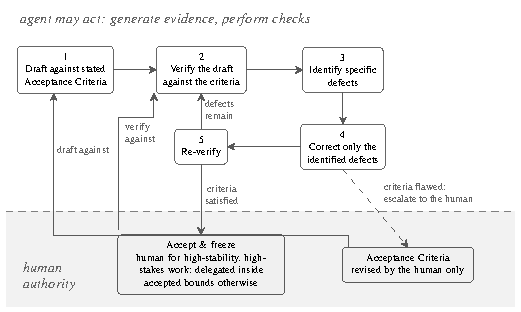
\includegraphics[width=\textwidth]{figures/f02/f02-verification-loop.pdf}
\caption{The verification loop of Verification-First Engineering, with the authority boundary drawn through it. Above the dashed line an AI agent may act: it drafts, verifies, identifies defects, corrects the identified defects, and re-verifies. Below the line sit the acceptance criteria and the accept-and-freeze decision. The human owner holds acceptance for high-stability or high-stakes work, and may delegate it inside accepted bounds otherwise. The criteria feed the draft and verify steps, and no step of the loop edits them: a criteria defect leaves the loop as an escalation to the human, who revises them.}
\label{fig:vloop}
\end{figure*}

Defining acceptance first fixes the target while it can still be stated plainly. Criteria written after a result exists are criteria the result has already shaped, and a failed check then returns a judgment rather than a named defect that correction can target.

The rule governs when acceptance is defined. It is not a claim that checking first produces better work: meta-analyses of test-first development in software report a small effect on quality, little effect on productivity, and mixed evidence overall \citep{rafique2013,munir2014}. The narrower claim is the one the principle carries. An artifact with no criteria written before it is an artifact whose definition of done can move.

Verification is performed by an executor or a context that did not produce the work \citep[Section~\hyperlink{nss-7.11}{7.11}]{pss2026}. That independence bounds a class of error and does not close it: independently produced versions of one program have been shown to fail together far more often than an assumption of independent failure predicts \citep{knight1986}. A second agent checking the first is a control with a known ceiling.

The reserve commitment is checkable before a single tank is sized. The criterion states an outcome the city must show: with the desalination plant stopped, the distribution network delivers water at the stated quality to every residential module for 72 hours. The method that will establish it is assigned when the obligation is written, and not after the design is underway \citep[Section~\hyperlink{nss-6.9}{6.9}]{pss2026}. It is chosen to fit the obligation, because the type of an obligation governs which method is admissible \citep[Section~\hyperlink{nss-6.6}{6.6}]{pss2026}. Where the physical check is expensive, slow, or irreversible, behavior is verified against a validated model first, and substituting the model for the check is a human decision recorded as one \citep[Section~\hyperlink{nss-7.16}{7.16}]{pss2026}.

Acceptance criteria and the definition of done belong to the human owner. An AI agent may draft against them, run the checks, produce the evidence, and correct the defects they identify. It may not alter them: disabling, deleting, or quietly weakening a criterion instead of satisfying it is a contract violation and not a shortcut \citep[Sections~\hyperlink{nss-7.2}{7.2} and~\hyperlink{nss-7.12}{7.12}]{pss2026}. An executor measured by a proxy for the thing that matters will move the proxy, which is a failure mode with a literature of its own \citep{skalse2022,manheim2018,specbench2026}. When the criteria are themselves wrong, the loop escalates and the human revises them.

Which artifacts need direct human acceptance is settled in advance rather than argued at the moment of change, and work sitting strictly inside already-accepted contracts and criteria may be accepted by automated checks \citep[Sections~\hyperlink{nss-7.10}{7.10} and~\hyperlink{nss-7.19}{7.19}]{pss2026}. Settling that list in advance is what makes the bound hold. Automation is misused or abandoned according to how well its limits are understood \citep{parasuraman1997}, and a limit settled at the point of change is a limit the change can argue with. Authority is granted the way a privilege is granted, at the least extent the work requires \citep{saltzer1975}, and it widens with the blast radius of the change \citep[Section~\hyperlink{nss-15.3}{15.3}]{pss2026}.

\subsection{Specifications as Contracts}

A specification that states required behaviors, interfaces, or acceptance criteria is a contract, and not advice \citep{tbf2026}.

The mechanism comes from design by contract, where a component's obligations are written as conditions that hold before a call, after it, and throughout its life \citep{meyer1992}. What the framework takes from it is the split rather than the notation: each component specification divides into a public contract, which is what other components may rely on, and a private design, which is how the component meets that contract and binds nobody else \citep[Sections~\hyperlink{nss-6.2}{6.2} and~\hyperlink{nss-6.3}{6.3}]{pss2026}.

That split decides which changes are local. Replacing the reverse-osmosis membranes with another vendor's is a private change, because the contract states the quality standard, the delivered volume, and the 72-hour reserve, and says nothing about which membranes produce them. Reducing the reserve from 72 hours to 48 is a changed obligation, whatever engineering argument supports it, because the 72 hours was committed to the authority that granted the permit.

The distinction does not follow the size of the work. A membrane replacement can take a year of fabrication and remain private, and an edit to one number in the reserve clause takes a minute and changes what the city owes. Effort is not the test. Whether anything outside the component was entitled to rely on the statement is the test.

A contract also carries the conditions under which it holds. An obligation that rests on an assumption states that assumption, so that a change in it surfaces as a reason to revise the contract rather than as a discovery years later. Each constraint is marked as externally imposed or internally owned \citep[Sections~\hyperlink{nss-6.5}{6.5} and~\hyperlink{nss-6.8}{6.8}]{pss2026}: the reserve duration is externally imposed and the reservoir siting is not, which is why one of them can be traded in a design review and the other cannot.

A contract is incomplete until it has been tested against cases meant to expose its gaps, its corner conditions, and its foreseeable misuse. Those cases are generated before acceptance, and the expanded contract binds on human approval and not before \citep[Section~\hyperlink{nss-6.14}{6.14}]{pss2026}.

Changing a contract requires a human decision. An AI agent may draft a revision and argue for it; it may not enact it. The authorities that no mechanism transfers are named rather than left to judgment: purpose, invariants and safety boundaries, acceptance criteria and the definition of done, risk acceptance, resource allocation, escalation, and any commitment with external consequences \citep[Sections~\hyperlink{nss-1.3}{1.3} and~\hyperlink{nss-15.2}{15.2}]{pss2026}. The commitment to the maritime authority is the last of those, which is why no local optimization of the water subsystem can reach it.

That division is carried by records and gates rather than by the wording of a standing instruction, because the priority of an instruction is not a control an agent can be relied on to preserve (Section~\ref{sec:related}). Each project names one responsible human for itself and for each component, and pairs that owner with an independent function charged with finding flaws \citep[Section~\hyperlink{nss-15.1}{15.1}]{pss2026}.

Taken together, the five principles put one demand on every unit of work: a boundary, a declared direction of dependency, a contract, criteria that decide when it is done, and a named human who owns the decisions those criteria encode. The cost of the set is writing. Every boundary, direction, separation, criterion, and commitment has to be recorded before a check can act on it, and a project that records none of them can still be built. What it cannot do is establish, three years later, which decision a proposed change is about to break. Section~\ref{sec:standard} turns these rules into the records and relations a project keeps, and states the checks that read them.

\section{Applying the Specification}\label{sec:standard}

\subsection{From patterns to clauses}

The 79 adopted forms were expressed as 106 numbered clauses, and every clause ends with a bracket that names the grounds it rests on.

Those brackets carry 183 links. Of them, 135 name an adopted form, 41 name one of the five principles, and 7 name a unit or a section of the goal document. A clause therefore stands on a mechanism, on a principle, or on the purpose I set for this work, and many stand on more than one.

The naming is structurally complete in both directions, and complete by computation rather than by assertion. Every one of the 106 clauses carries at least one link, at a mean of 1.73 and a maximum of 24. Every one of the 79 adopted forms is named by at least one clause, at a mean of 1.71 and a maximum of 6. Section~\ref{sec:results} reports the check that computes both.

The completeness is a property of the recorded grounding graph and nothing more. Every clause names grounds, and every adopted form is named by a clause. Whether a bracket names the right grounds is a separate question, settled by the clause-by-clause review of Section~\ref{sec:method} rather than by this count.

The clause carrying 24 grounds is the one that makes the minimum check set mandatory, and that spread is the point. A check set is where the rest of a normative document is enforced, so it inherits the grounds of everything it enforces.

One chain runs from a recorded practice to a check a reader can perform. The practice statement is that architecture decisions are kept as small numbered files beside the code they justify, under a fixed status vocabulary, and are never rewritten once accepted.

Generalization removed the software nouns and produced one adopted form. A binding decision is recorded as a numbered immutable record stating its context, the options considered with their trade-offs, the decision, its rationale, its consequences, and how compliance will be confirmed. Six other candidate statements were discarded into that one form.

Expression turned the form into four clauses on decision records and one on gate closure \citep[Sections~\hyperlink{nss-11.1}{11.1} to~\hyperlink{nss-11.4}{11.4} and~\hyperlink{nss-8.4}{8.4}]{pss2026}. The clauses fix what the record holds, the status vocabulary it draws from, the significance test that decides which decisions earn a record, and the rule that a reversal supersedes rather than edits.

The required record follows from the clauses: one decision record per binding decision, stored with the artifacts it governs. The check follows from the record: every record carries a status from the fixed vocabulary, and every supersession pointer resolves \citep[Section~\hyperlink{nss-16.2}{16.2}]{pss2026}.

What the chain buys is travel in both directions. A reader who doubts a clause reaches the practice statement it came from. A reader who changes an adopted form finds every clause that rests on it, which is the requirement of traversable consequence applied to this document.

External coverage of this family is one exploratory case study on the reuse of architecture decisions \citep{manteuffel2018}. That citation attributes a mechanism and validates no clause. No cited work supplied a clause.

Figure~\ref{fig:families} shows that the twelve mechanism families do not sit one to a section. Verification and acceptance reaches seven of the sixteen sections and contracts reaches six, because a rule about contracts constrains obligations, verification, baselines, and traceability alike. A reader who wants everything one family governs follows the brackets rather than the table of contents.

\begin{figure*}[t]
\centering
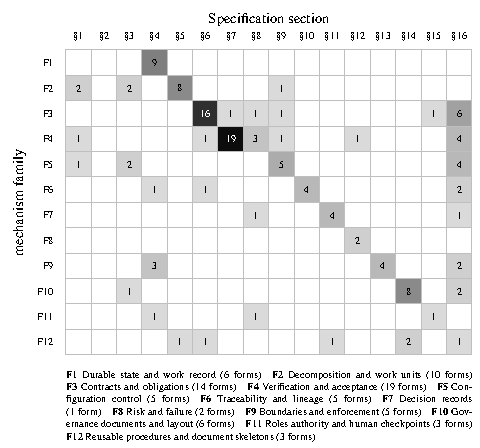
\includegraphics[width=\textwidth]{figures/f03/f03-family-section-matrix.pdf}
\caption{The twelve mechanism families against the sixteen sections of the Specification. A cell is marked where a clause of that section names a form of that family in its grounding bracket.}
\label{fig:families}
\end{figure*}

\subsection{Clause groups and their use}

The clauses fall into the twelve groups the twelve mechanism families produced: records, decomposition, contracts, verification, configuration, traceability, decisions, risk, executor limits, governance documents, authority, and procedures. Each group states a rule, requires a record or an action, and supports a check that reads what it required.

Records bind governing state to durable artifacts. Every state that governs work is a versioned artifact, with one canonical source per concern and any index over them generated rather than maintained by hand. The project record must be machine-readable. The check is blunt: an agreement that exists only in a session binds nothing. Provenance modelling supplies the shape such a record needs \citep{provdm2013}.

Decomposition binds work to units one executor can finish in one bounded effort. Each unit carries acceptance criteria and a declared blast radius, the set of elements it can affect \citep{kretsou2021}, and a unit whose blast radius cannot be bounded is split before it starts \citep[Section~\hyperlink{nss-5.6}{5.6}]{pss2026}.

Parallel units must have blast radii that do not overlap, because of what an overlap does to the estimate. Two units that can reach the same element bound nothing between them, since either can invalidate what the other was sized against. A defect in the shared element then belongs to no unit.

Two classes of unit are kept apart. A production unit changes the governed description under an approved plan. An exploratory unit runs in an isolated workspace with read-only access to the record, and nothing it produces governs anything. Work that proves out is redone as a production unit, and the exploratory record stays as evidence.

Contracts bind a component to what the rest of the system may rely on. Each component specification carries five sections a check can count: rationale, required behaviors, acceptance criteria, constraints, and dependencies and interfaces \citep[Section~\hyperlink{nss-6.2}{6.2}]{pss2026}. Each obligation is single, quantitative, and verifiable.

Each obligation also carries eight recorded attributes, among them a named human owner and the method that will verify it. An obligation missing one of them fails the check. Definition-of-done practice reports both the benefit of fixing completion that precisely and the difficulty of sustaining it \citep{kopczynska2022}.

Verification binds acceptance to text written before the work. The acceptance criterion and the verification method are authored with the obligation, and an obligation without a method does not enter an approved baseline. The executor that produced the work does not verify it.

Where one contract governs several realizations, one is designated the reference and compared with the others at a declared interval, so that divergence between what was specified and what was built is found on a schedule rather than at failure \citep{murphy2001}.

Configuration binds a description to a moment. Approved descriptions freeze as baselines, and one controlled gate governs every change to a locked one. A change re-issues the affected baseline entry and lands in the status ledger with an approving named human, a change class, and a marking of structural or behavioral \citep{iso15288}.

Traceability binds an obligation to the purpose above it and to the work below it. The links live in identifiers, naming, and placement, so any matrix over them is derived and never maintained by hand. The check refuses an obligation with no parent path to the vision document and one with no child path to realization elements and procedures. The backward direction is the one practitioners report as missing \citep{gotel1994}.

Decisions bind a choice to its reasons, and the chain above walks the group end to end. One rule reaches every other group: a decision record is the single home for the options considered and the rationale, and every other document points at it.

Risk binds an open exposure to a named closure. One register runs continuously, and a risk closes in exactly two ways, mitigated with evidence or accepted with a named human's rationale. The two are never recorded as one, because an accepted risk that reads as a mitigated one removes the grounds for revisiting it. Misuse and disuse of an automated control are documented failure modes, and a standing register is what keeps either one visible \citep{parasuraman1997}.

Executor limits bind an agent to a scope it cannot widen. Each executor's scope is declared once as a durable artifact, and its invariants are encoded as mechanical constraints rather than as prose, because a boundary that exists only as an instruction is a request \citep{saltzer1975}. Two rules follow: intermediate outputs are supervised for any attempt to weaken an acceptance criterion rather than meet it, and delegated work is isolated behind a condensed result.

Governance documents bind what an agent cannot discover from the system itself. One human-authored principles document states the reasoning the project applies, and every governance document stays under a declared size ceiling and references rather than copies. One study associates longer sessions with lower adherence \citep{mcmillan2026}, and the Specification therefore routes out of the document and into the versioned structure.

Authority binds every consequential judgment to a named human. One owner is named for the project, one for each component, and one for each obligation, and a standing function checks the work for flaws independently of whoever produced it. Seven authorities cannot be delegated: problem selection and purpose, invariants and safety boundaries, acceptance criteria and the definition of done, risk acceptance, resource and capital allocation, escalation decisions, and any commitment with external consequences, whether regulatory, financial, or contractual. AI agents may draft and propose in all seven and enact none of them.

Two consequences follow. The vision document and the governance documents are written and controlled by humans, because they carry purpose and reasoning rather than derived detail. The authority an action needs scales with its blast radius and with how hard it is to reverse \citep{parasuraman2000}.

Procedures bind recurring work to one definition. Work that recurs is written once as a reusable task definition: the steps in order, the acceptance criteria that close it, and the actions it forbids. Every design document spanning more than one work unit follows one skeleton and points at the decision records instead of restating them. The searched literature supplied no anchor for this group, which stands on the derivation record alone.

Four of the groups meet on one change. In the floating-city potable-water system of Section~\ref{sec:principles}, replacing a membrane module in the desalination train begins at the contract, in the obligation that fixes delivered water quality and names its owner and its verification method. Verification supplies the acceptance criterion and the procedure that tests it, and the agent that fitted the module does not run that procedure.

Traceability connects the work unit upward to the commitment made to the maritime authority and downward to the procedure that tests it, and the decision record holds why this membrane and not another. None of this requires reading the whole document. The reader finds the group, reads its clauses, and looks for the record the clauses name.

\begin{figure*}[!t]
\centering
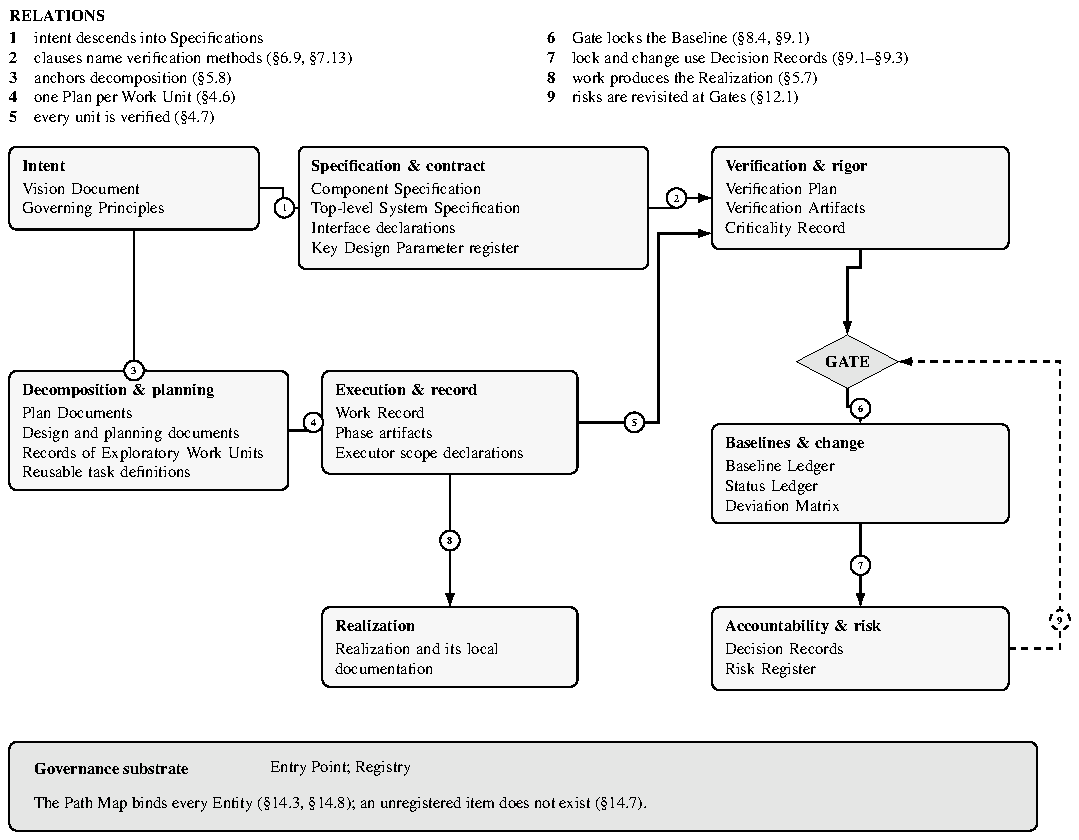
\includegraphics[width=\textwidth]{figures/f04/f04-entity-model.pdf}
\caption{The required Entities grouped by concern, with the relations the Specification declares between them. The governance substrate carries the Entry Point, whose Path Map binds every Entity to concrete storage, and the Registry, which holds the identity of every Component and content item. Drawn from the required Entity set of the Specification's \protect\hyperlink{nss-appA}{Appendix~A}.}
\label{fig:entities}
\end{figure*}

\subsection{Information model and reference binding}

A conforming project holds 24 required Entities, listed with their multiplicity in Table~\ref{tab:entities}. Figure~\ref{fig:entities} groups them by the concern each one serves and draws the relations between the groups. Intent reaches specifications, and specifications carry obligations that verification tests. Execution produces the record, baselines freeze what has been accepted, and decisions and risk attach to the baselines and the gates.

The model states which records must exist and how they refer to one another. It states nothing about where any of them lives, and the separation is deliberate \citep[Section~\hyperlink{nss-1.8}{1.8}]{pss2026}.

Four reasons hold it apart. A document that fixes file paths has confused its model with one storage of that model. Domains keep their records in their own formats, and a rule written for one format does not travel to another. Prose is the weakest artifact a check can read, so the binding has to name a format and not only a place. And a layout that serves one domain well is worth reusing rather than reinventing per project.

Each project declares a path map in its entry point that binds every required Entity to a location pattern and a serialization format. The binding is deterministic. An Entity with a multiplicity of one resolves to exactly one artifact, and for every artifact in the project record, its Entity is determinable from the map without judgement. The realization may sit outside the project record, wherever the map binds it, and the map declares its internal layout rather than classifying what is inside it. Checks resolve locations through the path map alone, so a check written once runs against a record laid out in any way the map can describe.

An Entity permitted zero instances is still bound. A project that runs no exploratory work unit binds that Entity to a pattern matching nothing, and the empty binding is what separates a project with no exploratory work from a project that lost the record of it.

One location is fixed, and it is the only one. The entry point is named \texttt{INDEX} and sits at the root of the project record, because a record whose map may be anywhere is not discoverable by anything that has not been told where to look.

Changing a locked description is not one act but a set of records, and which records depend on what changed. A change to a contract, an invariant, an acceptance criterion, or an artifact under human acceptance requires a new decision record. Every change to a locked baseline requires a status-ledger entry naming the re-issued snapshot, the approving human owner, the change class, and whether the change is structural or behavioral.

The affected baseline entry is then re-issued at the same locked status under the existing gate closure, and no new gate runs for a change that does not open one. Where the changed artifact is one the criticality record places under direct human acceptance, the change requires human authorization recorded in a decision record, and no automated procedure can supply it \citep[Sections~\hyperlink{nss-9.2}{9.2} and~\hyperlink{nss-7.19}{7.19}]{pss2026}.

Decision records are the one thing a change never edits. A superseded record keeps its text and gains a pointer from the record that replaced it, so the history stays readable in the order it happened.

The software profile offers one optional filesystem example. It uses Markdown for narrative records and JSON for structured records, with separate locations for specifications, plans, evidence, and registers. These choices illustrate how the required records can be stored; each project can select other locations and formats within the Specification.

A hardware profile gives a second optional example, for a physical system built from electronic, mechanical, and firmware components. The required records and their relations are the same as in the software example. What changes is the realization and its evidence. The built units are physical, so the example keeps their design and fabrication files in the formats of the design tools and describes each unit in an as-built record under its serial number. A bench measurement becomes a verification record that names the unit, the design release, and the instruments used. The domain changes the files and the evidence, while the required records and their relations stay the same. The example leaves domain-specific safety and regulatory practice to the methods and authorities of each domain.

A project that uses either example must complete its own path map and place every binding in its entry point. The local map must resolve without the external profile, including the locations and formats of the realization. Checks use that map and the declared format parsers, so changing storage preserves the required records and relations without making the example layout binding \citep[Section~\hyperlink{nss-14.8}{14.8}]{pss2026}.

\subsection{Scaled use and the minimum clause checks}

The smallest useful application is an ordered sequence and a short one. A vision document states the purpose. A criticality record fixes the class of the work and the reasoning for that class. An entry point declares the path map. One top-level specification carries the obligations, each with a named owner and a verification method. Decision records accumulate as binding choices are made, the ledgers and registers open empty, and the minimum checks run from the first day rather than from the first audit.

Every clause binds every project, and only depth scales. A two-person effort and a regulated capital programme both hold a contract, a verification method for each obligation, and a decision record for each binding choice. What the criticality class changes is how much evidence each one carries and how much independence its acceptance requires \citep[Sections~\hyperlink{nss-1.6}{1.6}, \hyperlink{nss-7.10}{7.10}, and~\hyperlink{nss-7.19}{7.19}]{pss2026}.

Scaling never reaches zero. An Entity is absent only through an entry in the deviation matrix naming what is waived, why, and which named human accepted the risk \citep[Section~\hyperlink{nss-1.5}{1.5}]{pss2026}. The matrix opens empty, so every absence in a conforming record is either declared or a defect.

A contained change shows the floor. Replacing the vendor of a chlorination setpoint controller in the floating-city water system touches one component, changes no obligation, and is recorded as a contained change in the status ledger against a re-issued baseline entry. No new gate runs and no acceptance is renewed, because the delivered water quality is unchanged and no commitment moved.

Shortening the 72-hour reserve is the same apparatus at a different depth. The reserve is an obligation the residents depend on and a commitment made to the maritime authority. The change therefore needs the authority to agree to a revised commitment, a decision record with the options and the accepted trade-offs, a re-issued contract, and a verification procedure that demonstrates the new figure. Acceptance is renewed by the named human owner, because a commitment with external consequences is not delegable \citep[Section~\hyperlink{nss-15.2}{15.2}]{pss2026}. Both changes use the same records. What differs is how many of them the change touches and how independent the acceptance has to be.

Sixteen checks are mandatory at minimum, and each one is written to detect a named class of defect. Six of them read the specification and its structure. They catch a specification missing one of its five sections, an unregistered component, and a registry entry that resolves to nothing. They catch an obligation without an owner or a verification method, and an obligation with no path upward to purpose or downward to work. They catch a circular dependency, a dependency on a less stable component, an acceptance criterion with no procedure, and a procedure with no clause.

The rest read the history and the substrate. They catch a decision record with an invalid status or a broken supersession pointer, a gate closed without a record, and a verification plan with no reference-realization designation or a designated contract with no comparison interval. They catch a baseline in an undeclared or dangling state, a locked baseline changed without a gate decision, and a change with no attribution or class. They catch a record with no discoverable entry point, a required Entity unbound or bound twice, and a governance document over its size ceiling. Table~\ref{tab:checks} states each check with the clause that imposes it and the defect class it detects.

A check that runs and leaves no trace does not count. The Specification states the rule as a flat sentence: ``A Normative Check whose outcome is not recorded has not run'' \citep[Section~\hyperlink{nss-16.3}{16.3}]{pss2026}. The outcome is itself a required record, which is what makes a result available to the next reader rather than only to whoever ran it.

The contract, configuration, and traceability records are what a change analysis reads. Section~\ref{sec:checks} states how a proposed edit is traced to everything it can affect, and that traversal runs over exactly these records.

Both requirements stated in the introduction are met by the same machinery. A clause carries its grounds, so a rule can be questioned without reconstructing why it exists. A record names what depends on it, so a change can be followed to its consequences before it is made. Section~\ref{sec:checks} turns the records into a representation a machine can traverse, and states what the traversal found.

\section{Representation and Checks}\label{sec:checks}

\subsection{Source-bound model}

The Specification stays prose, and the prose stays authoritative. A machine representation is derived from it, is rebuilt from it, and never replaces it. Every element of that representation names the bytes it came from, so a reader who doubts an encoded rule can open the sentence that produced it. The tool that builds and checks the representation is named Subspec, and this section reports what it represents, what it checks, and what it does not yet check.

The requirement unit is the sentence. A unit is identified by its document, its start byte, and its end byte, and that triple is its identity for every later stage. Sentence boundaries are computed by a deterministic segmenter, so the same source bytes always yield the same units. Nothing in the pipeline identifies a unit by its text, by its position in a list, or by a heading, because each of those changes when an unrelated edit lands above it.

Three products are derived from a requirement unit: propositions, typed relations, and classified gaps. A proposition is one obligation read out of one sentence. A typed relation is a named, directed link between two elements of the corpus. A classified gap is the recorded refusal to produce a proposition, carrying the reason for the refusal. A gap is a first-class result and not a silence, so an absent obligation is never read as an absent requirement.

A proposition carries an actor, a modality from a closed set, an action, a target, a precondition tree, an exception set, the quoted sentence, and its byte range. Section~\ref{sec:related} names the institutional grammar that is the nearest recorded ancestor of this shape. One component of that grammar has no counterpart in the Specification. The clauses state what must hold and never state the consequence of a breach, because that consequence belongs to the project that adopts the document. The mapping is otherwise direct, and the byte range is the provenance link that the general provenance model calls a derivation edge \citep{provdm2013}.

The corpus resolves into 3{,}853 source nodes across the four documents, arranged as a containment tree seven levels deep, and that set is the universe every change-impact answer partitions. Figure~\ref{fig:graph-structure} shows the tree aggregated by depth and node type. Semantic vocabulary adds further nodes for the actors, actions, entities, and defined terms that propositions refer to, and eleven edge types connect the whole. Section~\ref{sec:results} reports the sizes.

\begin{figure*}[!t]
\centering
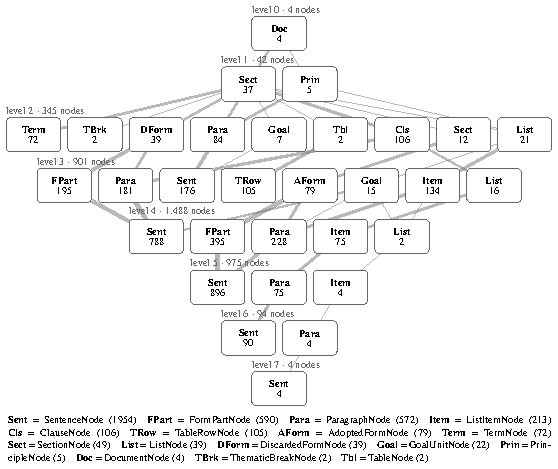
\includegraphics[width=\textwidth]{figures/f05/f05-graph-structure.pdf}
\caption{The containment tree of the corpus, aggregated to one chip per depth and node type. Each chip states the type abbreviation and its count at that depth; each line is the set of containment edges between two chips, drawn with a width proportional to the square root of the number of edges it carries. The row totals on the left sum to the 3{,}853 source nodes. The layout algorithm uses barycenter sweeps to place the groups without manual adjustment. The drawing aggregates: it shows where the corpus is deep and where it is wide, and it identifies no individual node.}
\label{fig:graph-structure}
\end{figure*}

The boundary between deterministic work and model-assisted work is drawn inside the pipeline and not around it. Figure~\ref{fig:pipeline} places it. Reading bytes, parsing CommonMark, building the typed intermediate representation, validating it, persisting it in one transaction, and running the link passes are pure functions of their input, with no model call and no database read. A model is invoked at one stage only, on one bounded unit at a time, under a pinned prompt, and its answer must satisfy a versioned schema before anything accepts it.

Six operations are closed to a model by construction. A model never assigns an identity, never parses structure, never resolves a cross-reference, never extends the controlled vocabulary, never evaluates a rule against a project state, and never decides a finding or a reachability answer. What a model contributes is an interpretation of one sentence, offered in a fixed shape. What turns interpretations into a recorded result is code and review together: code alone validates, canonicalizes, and persists them, and the semantic relations of the next subsection passed a review chain as well. The division matters for reproducibility. The deterministic stages replay from the source bytes at any time, and only the interpreted layer needs its recorded provenance to be trusted.

\begin{figure*}[t]
\centering
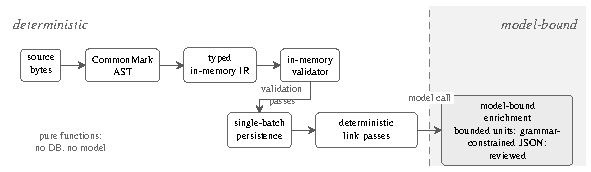
\includegraphics[width=\textwidth]{figures/f06/f06-ingestion-pipeline.pdf}
\caption{The ingestion pipeline and its determinism boundary. Left of the dashed line every stage is a pure function of its input, with no model call. The single model-bound stage on the right is entered one bounded unit at a time, with grammar-constrained output, a consensus check during calibration, and delegated review in production. The figure locates the boundary; the measurement methods and rebuild checks are in Appendix~\ref{app:repro}.}
\label{fig:pipeline}
\end{figure*}

The obvious alternative is to stop deriving and start authoring: write the rules in a formal language once, and generate the prose from them. That fails on the population this paper reports. Of 572 requirement units, 212 produced a classified gap rather than a proposition, mostly because the sentence names a concept the controlled vocabulary does not carry. A formal-first corpus would have had to either invent those concepts or leave the sentences out, and a sentence left out of the formal layer is a requirement with no record of its absence. Deriving from prose keeps the unrepresentable parts visible as counted gaps instead of absorbing them into a vocabulary that was never asked to cover them.

\subsection{Extraction and relation review}

Extraction ran over all 572 requirement units under one named single-lane evidence policy, with review and ratification delegated to an AI model. It compiled 360 of them and recorded a classified gap for the other 212, most of which name a concept the ratified vocabulary does not hold. Section~\ref{sec:method} states the fingerprint rule that governed calibration, and Section~\ref{sec:results} reports what the pass produced; this subsection states which passes ran under which policy.

Two things must not be confused at this stage. The controlled vocabulary is human work: I reviewed the candidate symbol registry symbol by symbol and ratified it on 2026-08-31, and no model may add to it afterwards. The semantic relations are not human work: they were proposed by a model, reviewed under delegated authority, and adjudicated by rule. Every artifact records which of the two it is, in its own metadata, so the standing of a number is read from the artifact and not from its surroundings.

Three relation passes produced the retained semantic edges, and the endpoint rules of each were frozen before it ran. The clause-to-goal pass put all 2{,}332 clause and goal-unit pairs to the lane, reviewed every answer case by case, and wrote 331 clause-to-goal links. The dependency pass covered the remaining 42{,}400 candidate pairs in 191 tiles and proposed 240 edges. A blind review of the 369 consequential answers, an adjudication that wrote 22 reusable rules, three judging rounds, and two seeded negative audits reduced those to 170 and overturned 75 pass answers. Two further rulings then judged the mutual pairs as pairs and the one remaining ring as a whole, removing 13 more and leaving 157 dependency links.

The candidate sets are checked as sets, not counted. The eligibility matrix is pinned by hash, and the two selections are derived from the frozen endpoint rule. The analysis layer refuses to call dependency coverage complete unless the registered passes cover the 44{,}732 candidates jointly and without overlap. Coverage of a candidate set is not correctness of its classifications, and the layer reports the two separately.

The two-stage shape is the one Section~\ref{sec:method} describes. Stage one calibrated the policy under dual-lane consensus on a ratified oracle and locked it. Stage two ran the corpus under reduced controls, with each pass carrying its own named policy and its own layered review. The tightening that would close the formal gate is a second production lane, and I deferred it on 2026-09-16 for time and budget reasons. The deferral changes no criterion. Every corpus-scale relation in this paper is delegated-AI single-lane evidence, and none of it is offered as dual-lane consensus or as human ratification.

\subsection{Deterministic analysis and change impact}

Five analysis operations read the graph without changing it. Verification runs the static checks over one database. Change-impact analysis partitions the corpus around a proposed edit. Change planning diffs two databases, or applies a mutation document to one, and emits the minimal ordered edit list. Derived export writes the coverage artifacts with a hash manifest. Source-change analysis compares the saved graph against the current source files. Every operation binds its output to its input through a database identity block. That block carries the file digest, the schema version, the corpus digest, the evidence policies, and both the recorded and the recomputed graph fingerprints. Repeated runs produce byte-identical output.

Verification runs seventeen named checks in four families. Integrity checks read the database itself: foreign keys, overall database integrity, dangling edge endpoints, duplicate relation edges, invalid endpoint types, and the validity of every stored rule against its schema. Coverage checks read the corpus: clauses with no implementing path, goal units with no inbound path, and the totals of the classified gaps. Consistency checks read the propositions: dangling condition references, directed cycles, and deontic clashes between an obligation and a prohibition whose guards can both hold. Provenance checks read the evidence: relation-edge provenance, the consistency of decisions with edges, the presence of dependency evidence, the incremental record, and authority leakage. The deterministic checks on defined terms follow the requirements-smell tradition \citep{femmer2017}, and the goal-coverage check descends from goal-oriented requirements analysis \citep{vanlamsweerde2001}.

Change impact analysis \citep{kretsou2021} is answered here as a partition and not as a list. The eligible universe is every source node. The seed nodes identify the elements selected for the proposed edit. Everything reachable from a seed over a propagating edge type, within the depth cap, is what the change may affect, and each entry carries its minimum depth over those edge types and a witness path whose steps record their direction. The rest of the universe is either proven unaffected or reported as blocked. Containment and document order do not propagate, because position in a document is not coupling.

A node enters the unaffected set only when two facts both hold. Dependency coverage must be complete, which establishes that every eligible dependency candidate in the defined universe has been classified under the registered policy, and the frontier must not be truncated, which establishes that the walk ended naturally rather than at the cap. Coverage alone is not enough: a walk cut short leaves the nodes past the frontier unexamined, and an unexamined node has not been proven to be anything. While either fact fails, the unaffected set is empty and every unreached node is reported as blocked. The rule is what stops the analysis from issuing a clearance it cannot support.

One change makes the behaviour concrete. Clause \hyperlink{nss-16.2}{16.2} of the Specification is the clause that makes the minimum check set mandatory, and Section~\ref{sec:standard} states that it names 24 grounds. A proposal to change it is seeded on that clause alone, and the analysis is run against the frozen dependency database at increasing depth caps. At depth 1 it reaches 45 nodes. At depth 2 it reaches 185, among them 94 of the 106 clauses, 30 of the 79 adopted forms, 13 goal units, and 4 of the 5 principles. At depth 4 it reaches 581, and the frontier is still truncated, so nothing is cleared. At depth 8 the walk converges: 1 node must change, 762 may be affected, 3{,}090 are proven unaffected under the recorded dependency graph, none are blocked, and the frontier is not truncated.

The converged answer is honest and of low discriminating value, and the reason is a property of this corpus rather than a defect of the method. The propagating graph is dominated by one large component, so a deep walk from almost any clause saturates it, and three unrelated seeds converge on the same 762 nodes. What the converged run establishes is the complement: 3{,}090 nodes lie outside the component and cannot be reached from this clause at any depth.

The useful reading is at the shallow depths, and the edge types that enter each depth say where it stops being useful. Every one of the 45 nodes at depth 1 is entered by a relation the clause itself asserts: 24 by its grounds, 15 by a recorded dependency, and 6 by an implementing link. The 140 added at depth 2 are entered the same way, by 66 implementing links, 44 explicit cross-references, 43 grounds, and 33 dependencies, and by nothing else; a node can be entered by more than one type. At depth 3 shared vocabulary appears, and at depth 4 it dominates: 236 of the 265 nodes added there are entered because two sentences use the same defined term. Two sentences that share a term are not thereby coupled. The depth-2 set of 185 is therefore the last one every member of which is reached by an asserted relation or an explicit reference, which is what makes it the review list rather than an arbitrary cut. The converged set stays useful as the outer boundary of what could ever matter.

Source-change analysis answers the same question from the other end. It compares the saved document bytes with the current files and reparses in memory. It reruns the term, reference, and appendix checks, and reports which findings are new and which are resolved. It identifies added, removed, and modified units from their full extents, and seeds the impact walk with those units and with the targets of the links inside them. A line shift alone changes nothing. The scope of its answer is stated in the report as the saved graph only, and any non-empty source difference sets a review flag, because a new dependency cannot be proven from old evidence. An unaffected verdict in the baseline partition is not a clearance for new meaning.

Change planning closes the loop by producing the edit rather than the diagnosis. Its input is a baseline and a candidate, or a baseline and a mutation document. It emits a deterministic ordered list of edit operations in a fixed group order. It also maps which findings the change introduces and which it resolves, and seeds a blast-radius run on the changed nodes. A locked regression fixture holds the method to that contract. For a goal deliverable with no inbound implementing path, the expected plan is exactly one added edge. The test replays that operation onto a scratch copy and reruns verification, and the targeted finding is resolved with no new error.

The practical result is the inspection path. When a clause changes, the traversal names the clauses that share its grounds, the adopted forms it descends from, the goal units it serves, the propositions extracted from it, and the terms it uses. Those are the contracts to reread, the records to reissue, and the checks to rerun. The list is produced by a query rather than by memory, it is the same list for every reader, and each entry carries the path that put it there.

\begin{figure*}[t]
\centering
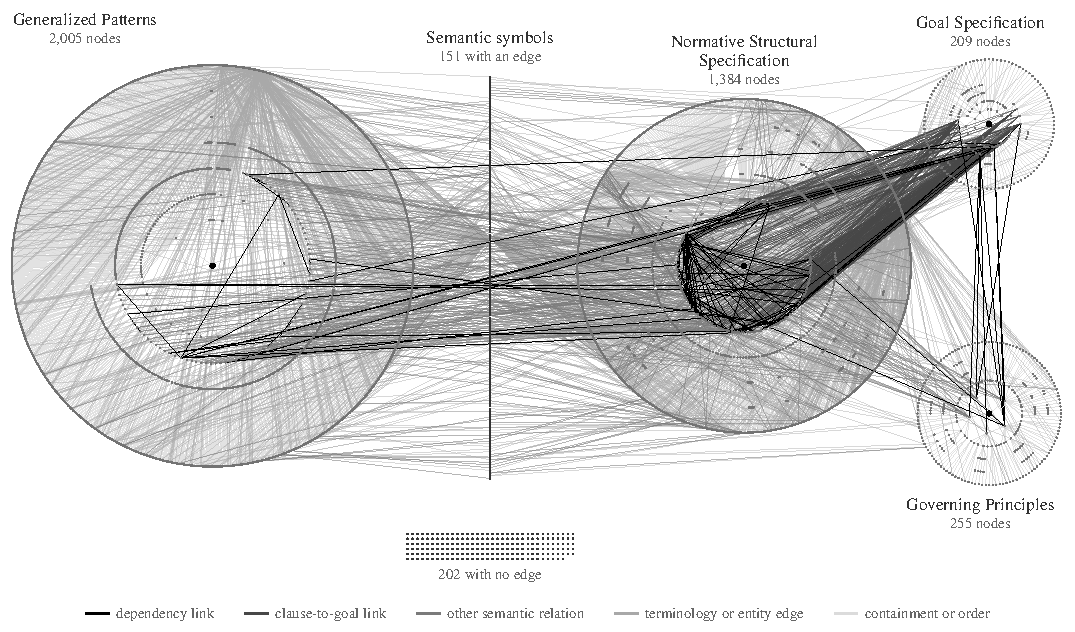
\includegraphics[width=\textwidth]{figures/f07/f07-semantic-graph.pdf}
\caption{The semantic graph in full: every one of the 4{,}206 nodes and every edge of the dependency database, recomputed 2026-09-21. No reduction is applied. Each document is one radial tree, and the area of each tree is proportional to its node count. Every leaf sits on the rim of its tree in document order, and each internal node sits at the mean angle of its children at a radius set by its depth, so containment reads as the spokes of a tree and document order as its rim. The Normative Structural Specification, which holds most of the relations, stands between Generalized Patterns and the two small documents, Governing Principles and the goal document. The 151 semantic symbols that carry an edge form the column between Generalized Patterns and the Specification, ordered by the mean height of their neighbours; the 202 that carry none form the grid below it, being the 157 actions the schema stores as proposition fields rather than as edges and 45 further ratified symbols that no proposition refers to. Structural and reviewed semantic edges are separated by gray tone, as the key shows: dependency links solid black, clause-to-goal links dark gray, other semantic relations middle gray, terminology and entity edges light gray, and containment and ordering edges the lightest gray. The 8{,}913 directed edges render as 8{,}905 undirected lines, because eight parallel pairs collapse into one line each. The relation edges are delegated-AI single-lane output under the review conditions described in Appendix~\ref{app:repro}: not human ratification, not dual-lane consensus, and not a closed gate.}
\label{fig:semantic-graph}
\end{figure*}

\subsection{Implemented checks and remaining limits}

The analysis used three successive databases: the extraction database, the relation database, and the dependency database. What each operation can conclude depends on which stage it reads. The first two lack complete dependency evidence, so their change-impact results clear no node as unaffected. The third records both relation passes and supplies the final dependency and verification results. Appendix~\ref{app:repro} states the input stage for each measurement. Verification passes on the dependency database under a ruling that lowers the 39 conflicts to informational severity and leaves them visible.

What stays open is reported rather than repaired, and nothing is closed by relabelling. Uncovered clauses, uncovered goal units, and extraction gaps all stay in the report at warning or informational severity. Four directed cycles stand by decision rather than by oversight, because the corpus states a mechanism and its own change control in one clause, and a rule that governs its own amendment is a cycle a reader should see. Section~\ref{sec:results} reports each finding against the artifact and the policy that produced it.

One implemented check has no active restrictions to enforce. Authority leakage is implemented and runs on every verification, and it reports nothing, because the ratified registry declares an empty actor-action binding list under an unrestricted policy. An empty list imposes no restriction, so the check has nothing to enforce. The twenty bindings a generator derived are benchmark evidence and not an authority matrix: they cover twenty of the 1{,}099 possible pairs of 7 actors and 157 actions, leave most actors unbound, and carry no clause-level provenance. Until a complete matrix is approved by a human, authority enforcement is specified and not active, and this paper claims it as neither.

The reserved work is therefore of two kinds. One is evidence: a second production lane would let the corpus-scale relations be reported as dual-lane consensus instead of reviewed single-lane output, and that gate stays open by decision. The other is capability: the authority matrix, and a scope repair that would let the 39 clashes be re-extracted rather than settled by ruling. Both are named as open in the project record, with the criteria that would close them unchanged.

The checker's schedule binds the checker and binds nothing else. The Specification requires a project to run a minimum set of sixteen normative checks over its own record, and Section~\ref{sec:standard} states that requirement and its deviation rule. Those checks are obligations on a project, and they are satisfied by whatever the project uses to run them. A check that this checker has not yet implemented is not a check a project may skip. The two sets are about different subjects: the checks reported in this section read four documents, and the checks the Specification mandates read a project record.


Figure~\ref{fig:semantic-graph} draws the whole graph at once, and its purpose is to connect the source model of this section to the analyses above it. The spokes are the containment tree that the parser produced deterministically from the bytes. The darker chords are the relations a model proposed and a review chain accepted. Reading the two classes apart is the point of the drawing: the structure is replayable from the source at any time, and the semantics carry the standing of the policy that produced them. Section~\ref{sec:results} reports what the checks found in that graph.

\section{Results}\label{sec:results}

\subsection{Complete grounding}

Every one of the 106 clauses of the Specification carries at least one recorded ground, and every one of the 79 adopted forms is cited by at least one clause. The 183 grounding edges close both directions, so no clause stands without a stated basis and no adopted form was collected and then left unused. Completeness in this sense is a property of the record and not of the argument: an edge states that a clause was written from that ground, and no check grades how well the clause serves it.

The grounds are not of one kind. Of the 183 edges, 135 reach an adopted form, 41 reach a frozen principle, 6 reach a goal unit, and 1 reaches a goal section. 96 of the 106 clauses name at least one adopted form, and the remaining 10 rest on a principle or on a stated goal alone. To call the layer a clause-to-pattern mapping would hide those 10 clauses, which are the ones whose basis is the project's own objective rather than collected practice.

The load is uneven on both sides. 64 clauses cite one ground, 31 cite two, 7 cite three, 3 cite four, and clause \hyperlink{nss-16.2}{16.2} cites 24, because it lists the mandatory checks and inherits the grounds of everything it checks. 45 of the 79 adopted forms are cited by one clause, 20 by two, 11 by three, 1 by five, and 2 by six. The clauses that cite a given adopted form are listed by a query over the grounding edges.

Table~\ref{tab:corpus} states the measured sizes of the corpus and its derived layers. Every count in it was recomputed on 2026-09-21 against the dependency database named in Appendix~\ref{app:repro}, opened read-only, and none was copied from an earlier working note.

\begin{table*}[t]
\centering
\caption{Measured properties of the corpus and its derived layers, recomputed 2026-09-21 against the fixed dependency database described in Appendix~\ref{app:repro}. The semantic relations are delegated-AI single-lane output under the review conditions described in Appendix~\ref{app:repro}, and are neither human ratification nor dual-lane consensus.}
\label{tab:corpus}
\begin{tabular}{p{2.1in}p{0.8in}p{3.5in}}
\toprule
Property & Count & Basis \\
\midrule
Source nodes & 3{,}853 & Deterministic parse of the four documents into a containment tree \\
\addlinespace
Nodes in total & 4{,}206 & Source nodes plus 353 ratified semantic symbols \\
\addlinespace
Directed edges & 8{,}913 & Eleven edge types, structural and semantic together \\
\addlinespace
Clauses, and clauses grounded & 106, 106 & Outbound grounding links per clause \\
\addlinespace
Adopted forms, and forms cited & 79, 79 & Inbound grounding links per adopted form \\
\addlinespace
Grounding edges & 183 & 135 to an adopted form, 41 to a principle, 7 to the goal document \\
\addlinespace
Requirement units & 572 & One sentence each, addressed by document and byte range \\
\addlinespace
Units compiled, and classified gaps & 360, 212 & Extraction status recorded per unit \\
\addlinespace
Propositions & 544 & Validated rule records from the 360 compiled units \\
\addlinespace
Clause-to-goal links & 331 & Reviewed clause-to-goal pass, 2{,}332 recorded decisions \\
\addlinespace
Clauses linked to a goal, goal units linked & 81 of 106, 17 of 22 & Distinct endpoints of the clause-to-goal links \\
\addlinespace
Dependency links & 157 & Tiled dependency pass with blind review and adjudication \\
\addlinespace
Semantic symbols, and symbols carrying an edge & 353, 151 & Ratified registry, and endpoint membership in the edge set \\
\bottomrule
\end{tabular}
\end{table*}

\subsection{Requirement representation and missing goal paths}

The corpus divides into 572 requirement units, of which 360 compiled into 544 validated propositions and 212 produced a classified gap. Figure~\ref{fig:coverage} shows the split and the composition of the gap set. A gap is a recorded refusal rather than a silent omission: each one names the unit, its byte range, the reason it could not be represented, and the remediation it would need.

\begin{figure*}[t]
\centering
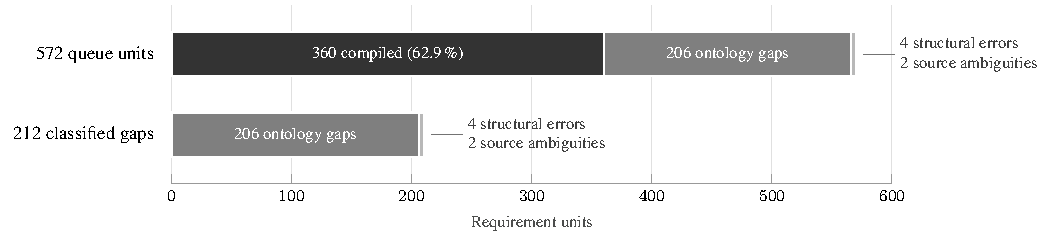
\includegraphics[width=\textwidth]{figures/f08/f08-coverage.pdf}
\caption{Representation coverage over the 572 requirement units. 360 units compiled into propositions and 212 were recorded as classified gaps, of which 206 are ontology gaps, 4 are structural errors, and 2 are source ambiguities. The abstention is explicit and addressable: each gap carries its unit, its byte range, and its required remediation.}
\label{fig:coverage}
\end{figure*}

Of the 212 gaps, 206 are ontology gaps, where the sentence names a concept the controlled vocabulary does not carry, 4 are structural errors, and 2 are source ambiguities. The gap population is therefore dominated by vocabulary coverage rather than structural failure or source ambiguity.

The modality field is concentrated in obligation. 432 of the 544 propositions are required actions, 85 are prohibited actions, 25 are permitted actions, and 2 are definitional, so 517 state an action that is required or forbidden and 27 do not.

The actor field is concentrated further. 504 of the 544 propositions bind the generic project actor, 13 bind an executor, 11 a human authority, 10 an AI agent, 2 a named human owner, 2 a declared role, and 2 carry no actor. The authority-leakage check exists to find an obligation placed on the wrong party, and on this corpus it has at most 40 propositions to rule on even after the authority matrix is populated.

Goal paths were built as a separate reviewed pass. 331 clause-to-goal links were retained from 2{,}332 recorded clause-and-goal decisions, under the named single-lane relation policy with delegated-AI ratification. Those edges are not human ratification and not dual-lane consensus, and the second lane over this pass is open by decision rather than by oversight.

81 of the 106 clauses reach at least one goal unit, and 25 reach none. A covered clause carries between 1 and 11 edges with a mean of 4.09, and a covered goal unit receives between 1 and 36 with a mean of 19.47. Figure~\ref{fig:relation-graph} shows the distribution of the edges by clause section and goal band.

\begin{figure}[t]
\centering
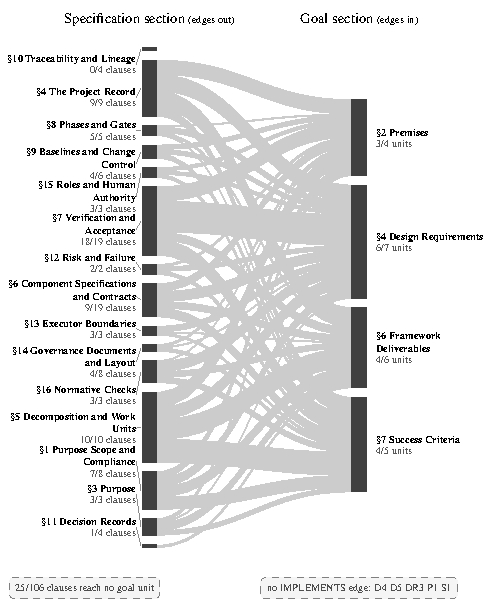
\includegraphics[width=\columnwidth]{figures/f09/f09-relation-graph.pdf}
\caption{The reviewed clause-to-goal relation, aggregated from 331 clause-to-goal links into bands between clause sections on the left and goal units on the right, with band thickness proportional to edge count. The edges are delegated-AI single-lane output under the production review conditions in Appendix~\ref{app:repro}. 25 of the 106 clauses appear on no band because no path to a stated goal was recorded for them.}
\label{fig:relation-graph}
\end{figure}

The 25 unlinked clauses are not scattered through the document. They are all four clauses of the traceability section, ten clauses of the component-specification section, four of the governance-document section, three of the decision-record section, and clauses \hyperlink{nss-1.4}{1.4}, \hyperlink{nss-7.10}{7.10}, \hyperlink{nss-9.5}{9.5}, and \hyperlink{nss-9.6}{9.6}. Most govern how the project record is organised, labelled, linked, or kept consistent, rather than what the engineered system must do.

The reverse direction is sparse for a different reason. 17 of the 22 goal units receive at least one inbound edge and 5 receive none. Two of the five are deliverables the project has not built, two are the requirement and the acceptance criterion for that unbuilt work, and one is a premise, which nothing should implement by kind.

Three readings of the 25 survive the evidence, and the record does not choose between them. The Specification may carry record-keeping machinery that no stated objective asked for. The goal document may be under-specified, so that real objectives exist but were never written as goal units. Or one review lane may have missed links that a second lane would find. A second lane restricted to those 25 clauses separates the third reading from the first two, and no cheaper evidence does.

\subsection{Dependency structure and graph size}

The dependency pass evaluated 42{,}400 ordered candidate cells and proposed 240 edges; the retained graph holds 157. 75 of the pass's 240 answers were overturned in review, so reading the pass output as the graph would have been wrong by roughly a third. Every retained edge carries at least two separate judgments: 127 carry two, 23 carry three, and 7 carry four. 131 were settled by a blind reviewer who agreed with the pass without seeing it, 11 at a third round, 7 at a second, 5 by adjudication, 2 by a final ruling, and 1 by an audit of the negatives.

The edges touch less of the corpus than their number suggests. 126 of the 212 possible endpoints appear in the graph, 85 as the source of an edge and 72 as its target. So a change to a clause outside that set has no recorded dependent, which is a statement about the pass and its scope and not a guarantee that nothing depends on the clause.

Four directed cycles were retained by decision rather than removed. Two adopted forms depend on each other, clauses \hyperlink{nss-9.1}{9.1} and \hyperlink{nss-9.2}{9.2} depend on each other, and two longer rings close through clauses \hyperlink{nss-9.3}{9.3} and \hyperlink{nss-9.5}{9.5}. A ruling judged each ring as a ring and kept it, because the baseline and change-control clauses genuinely define one another. These cycles are in the Specification's own semantic graph. They are not a violation of the rule that a project's component graph must be acyclic, which binds a project's decomposition and not a description of the document.

Figure~\ref{fig:dependency-structure} reduces the 103 clause-to-clause edges to relations between sections. The section order along both axes is computed by an exact minimum-backward-weight search over the inter-section weights, so the 8 backward edges that remain are a property of the data rather than of the section numbering or my choice of axis order. The reduction exposes roles that the edge list alone does not show: the normative-checks section sends 15 dependencies and receives none, the decision-record section receives 13 and sends 1, and the terminology and traceability sections neither send nor receive.

\begin{figure*}[tp]
\centering
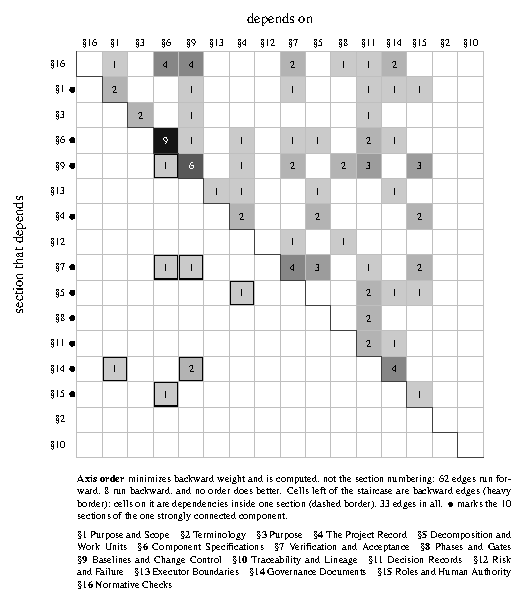
\includegraphics[width=\textwidth]{figures/f10/f10-dependency-structure.pdf}
\caption{The 103 clause-to-clause dependency links aggregated into an ordered section matrix, with 62 edges forward of the diagonal, 33 within a section, and 8 backward. The axis order minimises backward weight exactly, so the backward count measures the corpus and not the section numbering. The dependency links were produced by one model lane, then reviewed and adjudicated under delegated AI authority, with no human verification recorded on any edge.}
\label{fig:dependency-structure}
\end{figure*}

The whole graph holds 4{,}206 nodes and 8{,}913 directed edges across eleven types, drawn in Figure~\ref{fig:semantic-graph} as 8{,}905 undirected lines after eight parallel pairs collapse. 151 of the 353 semantic symbols carry an edge and 202 do not. The 202 resolve into 157 actions that the schema stores as a proposition field rather than as an edge, and 45 further ratified symbols that no proposition refers to. The worked change of Section~\ref{sec:checks} traverses this graph and marks 762 of the 3{,}853 source nodes as possibly affected.

\subsection{Corrections, clashes, and replay}

Verification of the final dependency database returns a pass with an exit code of zero over seventeen checks. Five checks report findings: 25 clauses with no outbound goal link and 5 goal units with no inbound one, at warning severity, 4 directed cycles at warning severity, 39 deontic clashes at informational severity under a recorded ruling, and the 212 extraction gaps at informational severity. Twelve checks report nothing, including database and foreign-key integrity, dangling endpoints, duplicate relation edges, relation provenance, and the validity of all 544 rule records.

The 39 clashes are the one finding class that a ruling moved. Each is a pair in which one proposition requires an action and another forbids it for the same actor and target. The ruling of 2026-09-17 records that every one of the 39 is raised by a restrictive prescription whose restricting complement the rule schema has no slot to hold. The pair is therefore an artifact of the representation and not one of 39 contradictions in the prose. The ruling lowers the severity to informational and leaves all 39 findings visible, and it does not assert that the clauses agree; it asserts that the schema cannot yet tell a conditional prohibition from an absolute one. The remedy it names is a schema slot, and until that slot exists the finding stays in the output.

The deterministic text checks hold 24 warnings in the final dependency database: 19 uses of a defined term in lower case, 4 capitalized phrases that no definition covers, and 1 defined term that nothing refers to. One finding of error severity was detected and repaired before this database was built. The hand-maintained coverage list in \hyperlink{nss-appB}{Appendix~B} of the Specification claimed five clauses for one principle where the generated list holds six, having omitted clause \hyperlink{nss-1.8}{1.8}. The source was corrected on 2026-09-17, and the finding is absent from the final dependency database while it remains in the two earlier ones.

Table~\ref{tab:findings} collects the findings of the whole programme with the procedure that detected each one and the action it produced. The construction findings of Section~\ref{sec:method} are carried in it, because a correction made during construction and a finding retained in the final analysis are both dispositions of the same record.

\begin{table*}[t]
\centering
\caption{Findings, dispositions, and the action each one produced. Graph findings were recomputed on 2026-09-21 against the final dependency database; construction counts are those of Table~\ref{tab:stages}.}
\label{tab:findings}
\begin{tabular}{p{1.05in}p{0.6in}p{1.6in}p{1.5in}p{1.42in}}
\toprule
Finding & Count & Detection procedure & Decision or correction & Resulting action \\
\midrule
Adopted forms needing revision & 21 of 79 & Isolated verification pass, three tests per form & Revised, then rechecked by a third model & Terminology set grew from 13 to 21 terms \\
\addlinespace
Rejected statements readmitted & 5 of 106 & Secondary rule on the recorded rejection reason & Readmitted, each with a written justification & 118 candidates entered generalization \\
\addlinespace
Support ratings on evidence & withdrawn & Evidence audit of the rating instrument & Ratings discarded after review and failed controls & No support rating is reported \\
\addlinespace
Coverage list omits a clause & 1 error & Comparison of the generated and written coverage lists & Source corrected 2026-09-17 & Finding absent from the final dependency database \\
\addlinespace
Deontic clashes & 39 & Conflict check over the 544 propositions & My ruling of 2026-09-17: one schema artifact & Severity lowered to informational, all 39 stay visible; schema slot required \\
\addlinespace
Clauses with no goal path & 25 of 106 & Clause-to-goal coverage check & Retained, unresolved & A second lane over the 25 is the next evidence \\
\addlinespace
Goal units with no inbound link & 5 of 22 & Inbound goal-link check & Retained; four cover unbuilt work, one is a premise & No change to the Specification \\
\addlinespace
Directed cycles & 4 & Cycle detection over recorded dependencies & Each ring judged as a ring and kept & Retained at warning severity \\
\addlinespace
Units with no proposition & 212 of 572 & Extraction gap queue, one entry per unit & Classified, each with its required remediation & 206 are vocabulary work on a known queue \\
\addlinespace
Terminology warnings & 24 & Lower-case use, undefined phrase, unreferenced definition & Retained as warnings & Retained in the analysis record \\
\bottomrule
\end{tabular}
\end{table*}

The internal rebuild test reproduced the relation graph exactly from its recorded decisions. The rebuilt graph had the same logical fingerprint as the original, and the two database files were byte-identical. A separate check recomputed the dependency database's fingerprint and confirmed its recorded value. Repeated derived exports were also byte-identical. The relation graph was rebuilt; the dependency database was not. These checks did not repeat the model calls behind the recorded decisions.

Replay settles reproduction and not acceptance. A rebuilt fingerprint shows that the same inputs and the same decisions give the same graph, and it says nothing about whether the purpose is the right purpose or the residual risk is tolerable. Those remain human decisions, and the record exists so that a person makes them against stated evidence rather than against a recollection.

The four source documents on disk have changed since the graph was frozen. A terminology rename on 2026-09-21 altered 24 requirement units across the four files. The change-detection command reports 507 seed nodes, no parse error, no new finding, and one finding resolved, and the digest table accepts the new bytes as terminology-only successors to the frozen ones. Every count reported above is therefore stated against the named frozen artifacts, whose digests are recorded, and not against the working copy.

Appendix~\ref{app:repro} binds the measurements to their input stages, counting rules, and review conditions. The internal rebuild checks establish repeatability from retained inputs and decisions. They do not establish independent reproduction or agreement between new model judgments.

\section{Discussion}\label{sec:discussion}

\subsection{What to use}

The first decision a project makes under the Specification is not which clauses to keep but how much evidence its work has to carry. That decision is the criticality class, scored for each component and each capability that spans components on failure consequence, complexity, human dependence, time to criticality, and exposure \citep[Section~\hyperlink{nss-7.10}{7.10}]{pss2026}. It is written before the records it governs, for the same reason acceptance criteria are: a class assigned afterwards is a class those records have already shaped, and it then approves whatever depth the work happened to reach.

What follows the class is a repeating unit of work rather than a plan. A unit is a bounded scope one agent can finish in one effort. Its criteria are written first, its blast radius is bounded before it starts, and any failure is repaired before the next unit begins \citep[Sections~\hyperlink{nss-5.5}{5.5}, \hyperlink{nss-5.6}{5.6}, and~\hyperlink{nss-5.9}{5.9}]{pss2026}.

The blast-radius step is where the record starts paying for itself. Before a change that touches earlier accepted work, the acceptance record states which criteria justified that acceptance, and the relations state what else the change reaches. A project without both rediscovers them by inspection. An agent working from one session's context cannot be relied on to rediscover them.

Most contained changes need neither a new decision record nor renewed acceptance. Replacing a chlorination controller in the floating-city water system changes no obligation, and a ledger entry against a re-issued baseline is the whole record. The same record structure governs a change to the 72-hour reserve, but that change reaches more records and requires stronger human acceptance.

The optional software layout gives a project a starting point for its path map. The project completes and checks the bindings for its own records, tools, and realization. Another layout must preserve the same required content and relations \citep[Sections~\hyperlink{nss-1.8}{1.8} and~\hyperlink{nss-14.8}{14.8}]{pss2026}. Verification evidence can be a saved test result, an inspection report, or a witnessed trial record, according to the domain. No corresponding layout example has been issued for a physical domain.

Scaling is a designed property of the document rather than a tolerated omission, which is what keeps it usable by a team of two. Lighter records are allowed, with the reason recorded against the criticality class, and an absent record is admissible only as a deviation entry that a named human accepted \citep[Sections~\hyperlink{nss-1.5}{1.5} and~\hyperlink{nss-1.6}{1.6}]{pss2026}.

Reusable task definitions are what stop the effort per unit from growing with the number of units. Work that recurs is written once as an ordered procedure with its criteria and its forbidden actions \citep[Section~\hyperlink{nss-5.10}{5.10}]{pss2026}. The second occurrence then costs a selection rather than a fresh specification, and the agent that runs it is bound by the text that bounded the first.

\subsection{What was measured}

Completeness of grounding is a property of the record and not a verdict on the rules. Nothing in those links grades how well a clause serves the ground it names. A reader who disagrees with a clause is nonetheless given the statement it came from, which is a different service from being told the clause is right, and the one a record can actually deliver.

What the representation adds is a set of questions a flat clause list leaves expensive. Which clauses rest on one mechanism family, which carry no recorded purpose, and which records need review after a proposed edit are answered by a query, and reading the document in order answers none of them.

The derivation chain answers the first of the two questions stated in the introduction: in this work, mechanisms used in practice became rules written to apply across domains through a chain in which each step keeps the record of the step before it. The grounding layer closing in both directions is the evidence that the chain was walked. One execution of a method is not that method's general behaviour, and the 21 forms that needed revision at first writing are the defect rate of this execution alone.

The findings answer the second question, and what they report is not what their labels suggest. The 39 flagged pairs all trace to one rule schema with no slot for the restricting part of a prescription, so they mark a limit of the representation rather than 39 contradictions in the prose.

The two requirements stated in the introduction are what these measurements test, and the Specification carries both on itself. Standing grounds is the grounding layer, complete in both directions. Traversable consequence is the traversal that names the clauses, forms, goals, propositions, and terms a proposed edit reaches.

The gap sits in a third relation rather than in either requirement. 25 of the 106 clauses carry no recorded link upward to a purpose, and that is the main place where the document does not yet meet what it asks of a project; the 24 terminology warnings of Section~\ref{sec:results} are the other.

Those 25 are not spread evenly, and the concentration is informative without being decisive. They fall almost entirely in the sections that govern how the project record is organised and kept consistent, rather than in those that govern the engineered system. The shape fits record-keeping machinery that no stated objective asked for, but a review lane that under-links clauses about the record itself would produce it too, and so would an under-specified goal document.

The effects of a proposed change appear as a partition of the corpus. In this corpus the propagating graph is dominated by one large component, so a deep walk from almost any clause reaches most of the others, and the converged answer says little. What a reviewer can act on is the shallow set reached by an asserted relation. The converged answer is useful for the set it shows untouched.

\subsection{Scope and next measurements}

Every number in this paper is a property of four documents. Whether the same construction, the same checks, and the same findings appear on another corpus is untested, and nothing in the measurements bounds that.

Grounding records a stated basis and assesses nothing. A bracket says a clause was written from a pattern, a principle, or a goal. No check asks whether the clause is a good expression of it, and no reader outside the project has been asked either.

The source population was chosen rather than sampled. I named the sources for each round and stopped collection when I judged that they supplied no further mechanisms, not when a measured coverage threshold was met. The 79 adopted forms therefore bound what was collected and not what practice contains.

The literature entered after the derivation and bounds the novelty claim rather than supporting the clauses. Only one cited work, ISO/IEC/IEEE 15288, also supplied a form. The per-form map was located by assisted search rather than by a registered protocol, and the instrument built to grade that map failed its controls and was withdrawn before use.

No score, ranking, or strength rating for any form appears in this paper. The map is evidence of positioning, and it is not evidence of coverage or of support.

The semantic relations carry the standing of the policy that produced them and no more. Each corpus-scale pass is delegated-AI single-lane output under its own named review policy, so a second production lane over the same candidate sets is the measurement that would show how stable those relations are under a second independent reading.

Independent readings of normative text may diverge substantially. In one study, three legally trained coders showed very low agreement when encoding the same statute independently; agreement improved when terminology was aligned and the encodings were formally validated \citep[Section~3]{witt2024}. This supports treating agreement as the product of an explicit review procedure rather than of independent reading alone.

The cheapest useful version of that measurement is restricted to the 25 unlinked clauses. It separates a missed link from a real absence, and no other evidence does.

The verification is self-referential, which is a limit of the evidence rather than of the tool. The mandatory check set descends from a clause of the document the checks read, so a blind spot in the document can be a blind spot in its checks.

Synthetic corpora engineered to trigger one defect each test the checks apart from the real corpus. They establish that each check fires; they do not establish that the set is complete.

Coverage of the logic layer is partial by design and must be read that way. 212 of the 572 requirement units carry a classified gap rather than a proposition, so a query over the propositions answers for the compiled 360 and is read against the coverage view.

The clauses are written for any domain: they name records and relations, and never a format or a tool. The software profile and a hardware profile for physical systems supply illustrative layouts. Neither profile is measured in this paper, and applying the hardware example to a real build is the next place to exercise that separation.

Nothing in this paper measures use. No project outside this work has adopted the Specification, and the aims the framework sets itself are unmeasured \citep{goal2026}. Internal verification evidence is what the artifacts support, and it is not evidence of effect.

Independent application is the next measurement, and it needs four answers rather than a verdict: whether a reader outside the project interprets a clause as it was written, whether the required records can be completed for a system the project did not design, whether acceptance decisions taken under the criticality classes survive review, and whether a change analysis names the records a domain expert would name.

A non-software binding is the setting that tests all four at once. It is the one place where the separation between the information model and its storage either holds or fails.

\section{Conclusion}\label{sec:conclusion}

The work produced five domain-general principles and the 106 numbered clauses of the Specification, which turn them into obligations a project can be checked against \citep{tbf2026,pss2026}. The clauses fix 24 required records and their relations. Each project declares its storage in a complete local path map, and optional software and hardware profiles supply filesystem examples.

In this work, mechanisms already used in practice became rules written to apply across domains, through a conversion in which every step keeps the record of the step before it. That answers the first of the two questions stated in the introduction. The conversion ran from 219 recorded practice statements through 79 domain-general forms to the clauses, each stage under its own control and with a recorded decision for every candidate.

What keeps the chain inspectable rather than asserted is the bracket at the end of every clause. Its links close in both directions: no clause stands without a stated basis, and no adopted form was collected and left unused.

Recorded grounds and relations answer the second question by separating three things a flat document holds together: missing support, conflicting requirements, and the reach of a proposed change.

Recorded grounding is complete and purpose is not. Most of the 25 clauses without a recorded path to a stated goal govern how the project record is organised rather than what an engineered system must do.

The conflicts are a property of the representation. All 39 flagged pairs trace to one missing slot in the rule schema, which cannot yet hold the restricting part of a prescription.

The reach of a change comes back as a partition. A proposed edit to the clause that mandates the minimum check set names 185 source nodes at the last depth reached only by an asserted relation or an explicit reference. It also proves 3{,}090 of the 3{,}853 source nodes unreachable from that clause at any depth.

The relation graph rebuilds from its recorded decisions to the same logical fingerprint, and the rebuilt file is byte-identical to the recorded one. Repeatability from recorded decisions is what that establishes, over four documents whose corpus-scale relations are delegated-AI single-lane output rather than human ratification. Whether the purpose is the right purpose, and whether the residual risk is tolerable, stay with the responsible human.

The two requirements stated in the introduction are carried by the Specification on itself, as a grounding layer complete in both directions and a traversal that names what an edit reaches. One relation falls short. Those 25 clauses are requirements whose purpose the document does not record, which is the thing it asks every project to record.

Four parts of the framework are named in its goal document and not built: the AI-native execution methods, the domain playbooks, the onboarding path, and the templates and checklists \citep{goal2026}. None of them is reported in this paper.

Independent application is the next measurement of the Specification. Until it runs, the evidence stated in this paper is internal to the work: the derivation is recorded, the methods and findings are reported with their review conditions, and its effect on a project is unmeasured.

\section*{Statement on AI use}

AI agents performed the construction and extraction passes of this study, and assisted the drafting of this paper. They collected the 219 source statements and screened each one in isolation, generalized the 118 candidates that entered that stage, and ran the passes that verified and corrected the result. They wrote a findings report for each of the 106 clauses, ran extraction over all 572 requirement units, and judged all 44{,}732 candidate relation pairs.

I set the problem, wrote the rules each pass ran under, reviewed the construction records, resolved the conflicts, and accepted or rejected every construction result. I delegated the review of the corpus-scale relation decisions to AI models. Section~\ref{sec:method} states, for each construction stage, who performed it and the control that bounded it, and Appendix~\ref{app:repro} pins the model identities that a reported result depends on.

I take full responsibility for the content of this paper, including every part an AI agent produced.

No AI system selected the research problem, set an acceptance criterion, or accepted this text. AI systems, among them GPT-6 Astra and Fable~5.1, did produce, review, and adjudicate findings and relation decisions under authority delegated by the author. Wherever those results bear on a reported result, the evidence policy named in Section~\ref{sec:method} records that standing explicitly.

No AI system is listed as an author. Accountability for a paper rests on a person who can answer for it, and a tool cannot hold it.

\section*{Data and artifact availability}

The goal document, framework, and Specification are issued as separate technical reports \citep{goal2026,tbf2026,pss2026}, and the software and hardware profiles summarized in Appendix~\ref{app:entities} are issued with the framework. Appendix~\ref{app:coverage} lists the 79 patterns and their clause mappings. Appendix~\ref{app:repro} describes the measurement inputs, counting rules, review conditions, and internal rebuild checks.

The reported rebuild results describe tests performed within this work.

\section*{Funding}

This work was funded by the author.

\section*{Conflicts of interest}

The author wrote the framework that this paper describes. The author declares no other conflict of interest.


\clearpage
\begingroup
\raggedright
\setlength{\bibsep}{0pt}
\setlength{\parskip}{0pt}
\bibliography{references}
\endgroup

\appendix
\onecolumn
\clearpage
\renewcommand{\thetable}{\thesection.\arabic{table}}
\renewcommand{\theHtable}{\thesection.\arabic{table}}
\renewcommand{\thefigure}{\thesection.\arabic{figure}}
\renewcommand{\theHfigure}{\thesection.\arabic{figure}}
\makeatletter
\renewcommand\@seccntformat[1]{\@nameuse{appx@cnt@#1}}
\newcommand\appx@cnt@section{Appendix~\thesection:\ }
\newcommand\appx@cnt@subsection{\thesubsection\quad}
\newcommand\appx@cnt@subsubsection{\thesubsubsection\quad}
\newcommand\appx@cnt@paragraph{\theparagraph\quad}
\newcommand\appx@cnt@subparagraph{\thesubparagraph\quad}
\makeatother
\sloppy
\hbadness=10000
\vbadness=10000

\setlength{\multicolsep}{4pt}
\setlength{\LTcapwidth}{\textwidth}
\setlength{\LTpre}{4pt}
\setlength{\LTpost}{4pt}
\setlength{\LTleft}{\fill}
\setlength{\LTright}{\fill}
\raggedbottom%
\small
\renewcommand{\arraystretch}{0.95}
\begin{multicols}{2}
\section[Required Entity Set, Glossary, and Reference Layout]{Required Entity Set, Glossary, and\\Reference Layout}
\label{app:entities}
\setcounter{table}{0}
\setcounter{figure}{0}

\subsection{Required records}

Table~\ref{tab:entities} lists the required records and their multiplicities from version~1.0 of the Specification \citep[\hyperlink{nss-appA}{Appendix~A}]{pss2026}. Their authority comes from that document. The clause references are a lookup aid, and the groups follow Figure~\ref{fig:entities}.
\end{multicols}

\begingroup
\footnotesize
\begin{longtable}{@{}p{0.28\textwidth} p{0.54\textwidth} p{0.12\textwidth}@{}}
\caption{The 24 required Entities of the Specification's \protect\hyperlink{nss-appA}{Appendix~A}, grouped by the concern each Entity serves.}
\label{tab:entities} \\
\toprule
Entity & Multiplicity & Clause \\
\midrule
\endfirsthead%
\multicolumn{3}{@{}l}{\tablename~\thetable{} (continued)} \\
\toprule
Entity & Multiplicity & Clause \\
\midrule
\endhead%
\multicolumn{3}{@{}l}{\emph{Intent}}\\
Vision Document & one & \hyperlink{nss-3}{\S3} \\
Governing Principles & one & \hyperlink{nss-14.1}{\S14.1} \\
\midrule
\multicolumn{3}{@{}l}{\emph{Specification and contract}}\\
Component Specification & one per Component & \hyperlink{nss-6.1}{\S6.1} \\
Top-level System Specification & one & \hyperlink{nss-6.17}{\S6.17} \\
Interface declarations & one per interface; those internal to a Component Specification are bound with it, those spanning Components are separately bound & \hyperlink{nss-6.10}{\S6.10} \\
Key Design Parameter register & one & \hyperlink{nss-6.18}{\S6.18} \\
\midrule
\multicolumn{3}{@{}l}{\emph{Decomposition and planning}}\\
Plan Documents & one per Work Unit & \hyperlink{nss-4.6}{\S4.6}, \hyperlink{nss-5.9}{\S5.9} \\
Design and planning documents & one per effort spanning more than one Work Unit; none where no such effort exists & \hyperlink{nss-6.19}{\S6.19} \\
Records of Exploratory Work Units & one per Exploratory Work Unit; none where no Exploratory Work Unit is run & \hyperlink{nss-5.7}{\S5.7}, \hyperlink{nss-6.13}{\S6.13} \\
Reusable task definitions & one per recurring kind of work & \hyperlink{nss-5.10}{\S5.10} \\
\midrule
\multicolumn{3}{@{}l}{\emph{Verification and rigor}}\\
Verification Plan & one & \hyperlink{nss-7.9}{\S7.9} \\
Verification Artifacts (Gate records, drift reports, quality record chain, Verification Reference State records, etc.) & one per verification event; element-local Verification Procedures live on the governed artifact & \hyperlink{nss-7}{\S7}, \hyperlink{nss-8.4}{\S8.4}, \hyperlink{nss-14.6}{\S14.6} \\
Criticality Record & one & \hyperlink{nss-7.10}{\S7.10} \\
\midrule
\multicolumn{3}{@{}l}{\emph{Execution and record}}\\
Work Record & one & \hyperlink{nss-4.5}{\S4.5} \\
Phase artifacts & at least one per Phase & \hyperlink{nss-8.1}{\S8.1} \\
Executor scope declarations & one per Executor & \hyperlink{nss-13.1}{\S13.1} \\
\midrule
\multicolumn{3}{@{}l}{\emph{Baselines and change}}\\
Baseline Ledger & one & \hyperlink{nss-9.1}{\S9.1} \\
Status Ledger & one & \hyperlink{nss-9.3}{\S9.3} \\
Deviation Matrix & one & \hyperlink{nss-9.4}{\S9.4} \\
\midrule
\multicolumn{3}{@{}l}{\emph{Realization}}\\
Realization and its local documentation & one Realization; internal layout declared in the Path Map & \hyperlink{nss-14.8}{\S14.8} \\
\midrule
\multicolumn{3}{@{}l}{\emph{Accountability and risk}}\\
Decision Records & one per binding decision & \hyperlink{nss-11}{\S11} \\
Risk Register & one & \hyperlink{nss-12.1}{\S12.1} \\
\midrule
\multicolumn{3}{@{}l}{\emph{Governance substrate}}\\
Entry Point & one & \hyperlink{nss-14.3}{\S14.3} \\
Registry & one & \hyperlink{nss-14.7}{\S14.7} \\
\bottomrule
\end{longtable}
\endgroup

\begin{multicols}{2}
\subsection{Terms used in the analysis}

Table~\ref{tab:glossary} defines the terms used to describe the derivation and the machine representation. Record names defined by the Specification retain their meanings.
\end{multicols}

\begingroup
\footnotesize
\begin{longtable}{@{}p{0.25\textwidth} p{0.69\textwidth}@{}}
\caption{Terms used in the derivation, information model, and graph analysis.}
\label{tab:glossary} \\
\toprule
Term & Meaning \\
\midrule
\endfirsthead%
\multicolumn{2}{@{}l}{\tablename~\thetable{} (continued)} \\
\toprule
Term & Meaning \\
\midrule
\endhead%
Pattern (\hyperlink{gp-01}{GP-01} to \hyperlink{gp-79}{GP-79}) & A mechanism taken from recorded practice and restated in domain-general form. \\
Merged candidate (D-01 to D-39) & A candidate whose mechanism is carried by one or more named patterns. \\
Requirement unit & A source sentence submitted for representation as one or more machine-readable propositions. \\
Information model & The required record types and their relations, defined independently of storage. \\
Path Map & The project's declaration of the location and format of each required record type. \\
Reference file layout & An illustrative arrangement of record locations and formats, adapted into a project's complete local Path Map. \\
Machine representation & A graph linking source text, extracted propositions, vocabulary, and recorded relations. \\
Grounding link & An explicit link from a clause to a pattern, principle, or goal that it names as its basis. \\
Clause-to-goal link & A reviewed relation stating that a clause serves a unit of the goal document. \\
Recorded dependency & A reviewed relation stating that one unit cannot be read or applied without another. \\
Flagged conflict between obligations & A pair of represented propositions that require and prohibit the same action for the same actor and target under compatible conditions. \\
Criticality Record & The register that assigns a criticality class to each component and capability. \\
Deviation Matrix & The register of accepted departures from binding clauses, with the recorded acceptance of each departure. \\
\bottomrule
\end{longtable}
\endgroup

\begin{multicols}{2}
\subsection{Optional filesystem example}

The required record types in Table~\ref{tab:entities} come from the Specification. Table~\ref{tab:layout} illustrates one way to store them, using the software profile, version~0.8. Its Markdown and JSON choices are examples. A project can choose other formats that its tools can read and check, while retaining the required content, relations, history, and human authority \citep[Sections~\hyperlink{nss-1.8}{1.8} and~\hyperlink{nss-4}{4}]{pss2026}.

The example places a documentation directory beside the software realization under the same version control. Paths in the table start at the documentation root. A project must adapt these bindings, complete the realization layout, and state the full Path Map in its Entry Point. An external profile reference with a list of exceptions is insufficient \citep[Section~\hyperlink{nss-14.8}{14.8}]{pss2026}. The Specification fixes only the Entry Point's root location and \texttt{INDEX} name; its extension follows the chosen format \citep[Section~\hyperlink{nss-14.3}{14.3}]{pss2026}.

An embedded interface has its own identifier inside its containing specification. The connected specifications refer to one canonical declaration. Phase records describe outputs through versioned references, and verification records point to the Decision Record that closes a Gate. These links preserve each record's role without copying its governing content. Registry locations are derived from the stored artifacts, so moving a record does not require a manually edited location entry \citep[Sections~\hyperlink{nss-4.3}{4.3}, \hyperlink{nss-8.4}{8.4}, and~\hyperlink{nss-14.7}{14.7}]{pss2026}.

The table is an example to complete, not a conformance result. A project also binds supporting records, local governance, procedure code, and evidence attachments, and declares their formats. Its Entry Point states the Stability Classes, decision significance test, Baseline levels and lock Gates, and change classification dimensions. The required checks and human reviews apply to the resulting project record \citep[Sections~\hyperlink{nss-14.3}{14.3} and~\hyperlink{nss-16}{16}]{pss2026}.
\end{multicols}

\begingroup
\footnotesize
\begin{longtable}{@{}p{0.30\textwidth} >{\raggedright\arraybackslash}p{0.43\textwidth} p{0.21\textwidth}@{}}
\caption{One optional filesystem arrangement from software profile version~0.8. Paths and formats are illustrative; each project completes its own local Path Map.}
\label{tab:layout} \\
\toprule
Entity & Example location pattern & Example format \\
\midrule
\endfirsthead%
\multicolumn{3}{@{}l}{\tablename~\thetable{} (continued)} \\
\toprule
Entity & Example location pattern & Example format \\
\midrule
\endhead%
Vision Document & \texttt{VISION.md} & Markdown \\
Governing Principles & \texttt{PRINCIPLES.md} & Markdown \\
Entry Point & \texttt{INDEX.md} & Markdown \\
Registry & \texttt{REGISTRY.json} & JSON \\
Component Specification & \texttt{components/*/SPEC.md} & Markdown \\
Top-level System Specification & \texttt{system/SPEC.md} & Markdown \\
Interface declarations & identified sections in the Component or System Specification; standalone declarations at \texttt{interfaces/*.md} & Markdown \\
Decision Records & \texttt{decisions/*.md} & Markdown \\
Records of Exploratory Work Units & \texttt{experiments/records/*.json} & JSON \\
Work Record & \texttt{work/record.json} & JSON \\
Plan Documents & \texttt{plans/units/*.md} & Markdown \\
Phase artifacts & \texttt{phases/*.md} & Markdown \\
Design and planning documents & \texttt{plans/designs/*.md} & Markdown \\
Verification Plan & \texttt{verification/PLAN.md} & Markdown \\
Verification Artifacts & \texttt{verification/events/*.json}; attachments have separate bindings & JSON \\
Baseline Ledger & \texttt{registers/baselines.json} & JSON \\
Risk Register & \texttt{registers/risks.json} & JSON \\
Status Ledger & \texttt{registers/status.json} & JSON \\
Deviation Matrix & \texttt{registers/deviations.json} & JSON \\
Key Design Parameter register & \texttt{registers/parameters.json} & JSON \\
Criticality Record & \texttt{registers/criticality.json} & JSON \\
Executor scope declarations & \texttt{scopes/*.md} & Markdown \\
Reusable task definitions & \texttt{procedures/*.md} & Markdown \\
Realization and its local documentation & \texttt{../realization/}; internal layout completed by the project & declared native formats \\
\bottomrule
\end{longtable}
\endgroup

\begin{multicols}{2}
\subsection{Optional hardware example}

The hardware profile, version~0.8, applies the same record bindings to a physical system built from electronic, mechanical, and firmware components. Each component has its own specification and design sources, and a larger system adds components under the same patterns. Table~\ref{tab:hwlayout} lists only the bindings that differ from Table~\ref{tab:layout}.

The built units are the realization, and a physical unit has no path. No check can read the unit itself; a check reads only its description. The Specification already treats a physical realization this way: a phase that produces realization is recorded through its description, and a Baseline freezes the description, never the realization \citep[Sections~\hyperlink{nss-8.1}{8.1} and~\hyperlink{nss-9.1}{9.1}]{pss2026}. The example therefore binds the design sources, fabrication files, and firmware in the realization directory, and its declared realization layout represents each unit only by an as-built record under its serial number \citep[Section~\hyperlink{nss-14.8}{14.8}]{pss2026}.

The device is fabricated, so the Entry Point declares an as-built Baseline level beside the functional and allocated levels. A bench measurement is a verification record that names the unit, the design release, and the instruments used. A reading that was not saved is not evidence \citep[Sections~\hyperlink{nss-7.18}{7.18} and~\hyperlink{nss-9.1}{9.1}]{pss2026}.

The example does not supply domain-specific safety, regulatory, or approval practice, which remains with the methods and authorities of each domain. It has not been applied to a build.
\end{multicols}

\begingroup
\footnotesize
\begin{longtable}{@{}p{0.30\textwidth} >{\raggedright\arraybackslash}p{0.43\textwidth} p{0.21\textwidth}@{}}
\caption{Bindings in hardware profile version~0.8 that differ from Table~\ref{tab:layout}. All other record bindings are unchanged. Paths and formats are illustrative; each project completes its own local Path Map.}
\label{tab:hwlayout} \\
\toprule
Artifact & Example location pattern & Example format \\
\midrule
\endfirsthead%
\multicolumn{3}{@{}l}{\tablename~\thetable{} (continued)} \\
\toprule
Artifact & Example location pattern & Example format \\
\midrule
\endhead%
Realization: stored part & \texttt{../realization/} with \texttt{electronics/*/}, \texttt{mechanical/*/}, and \texttt{firmware/*/} per component, plus \texttt{bom/} and \texttt{releases/} & design-tool native formats and firmware source \\
Realization: physical units & one as-built record per serial number at \texttt{production/units/*.json} & JSON \\
Bill of materials & \texttt{../realization/bom/*.csv} & CSV \\
Fabrication release packages & \texttt{../realization/releases/*/}, each with a digest manifest & Gerber, drill, and STEP or STL exports \\
Supplier and process records & \texttt{production/suppliers/*.md} and \texttt{production/process/*.md} & Markdown \\
Bench evidence attachments & \texttt{verification/data/**/*.csv} and photographs in the same tree & CSV, JPEG, PNG \\
\bottomrule
\end{longtable}
\endgroup

\clearpage
\begin{multicols}{2}
\section{Pattern Traceability and Derivation Ledger}
\label{app:coverage}
\setcounter{table}{0}
\setcounter{figure}{0}

Tables~\ref{tab:forms}--\ref{tab:forms-c} map each of the 79 patterns to the clauses that name it as a ground. Table~\ref{tab:principles} gives the same coverage for the five principles. The mappings are derived from the explicit grounding links in the Specification. Pattern names follow Generalized Patterns; principle names follow Governing Principles. Every pattern and principle has at least one recorded clause link.

Grounding and purpose are separate relations. Under the delegated AI review described in Appendix~\ref{app:repro}, 81 of the 106 clauses have a recorded link to a stated goal and 25 have none. The unlinked clauses are \hyperlink{nss-1.4}{\S1.4}, \hyperlink{nss-6.3}{\S6.3}, \hyperlink{nss-6.4}{\S6.4}, \hyperlink{nss-6.6}{\S6.6}, \hyperlink{nss-6.8}{\S6.8}, \hyperlink{nss-6.11}{\S6.11}, \hyperlink{nss-6.12}{\S6.12}, \hyperlink{nss-6.15}{\S6.15}, \hyperlink{nss-6.16}{\S6.16}, \hyperlink{nss-6.17}{\S6.17}, \hyperlink{nss-6.18}{\S6.18}, \hyperlink{nss-7.10}{\S7.10}, \hyperlink{nss-9.5}{\S9.5}, \hyperlink{nss-9.6}{\S9.6}, \hyperlink{nss-10.1}{\S10.1}, \hyperlink{nss-10.2}{\S10.2}, \hyperlink{nss-10.3}{\S10.3}, \hyperlink{nss-10.4}{\S10.4}, \hyperlink{nss-11.2}{\S11.2}, \hyperlink{nss-11.3}{\S11.3}, \hyperlink{nss-11.4}{\S11.4}, \hyperlink{nss-14.2}{\S14.2}, \hyperlink{nss-14.3}{\S14.3}, \hyperlink{nss-14.5}{\S14.5}, and \S14.7. Of the 22 goal units, 17 have an inbound clause link; D4, D5, DR3, P1, and S1 have none. These are gaps in the recorded relations, not proof that the clauses have no purpose.
\end{multicols}

\begingroup
\footnotesize
\begin{longtable}{@{}p{0.07\textwidth} p{0.43\textwidth} r p{0.34\textwidth}@{}}
\caption{Pattern traceability, part 1 of 3 (\protect\hyperlink{gp-01}{GP-01} to \protect\hyperlink{gp-27}{GP-27}). Names are source headings, and each mechanism is my one-sentence summary of the pattern; clause links are generated from the graph.}
\label{tab:forms} \\
\toprule
Pattern & Name and mechanism & Clauses & Realized in \\
\midrule
\endfirsthead%
\multicolumn{4}{@{}l}{\tablename~\thetable{} (continued)} \\
\toprule
Pattern & Name and mechanism & Clauses & Realized in \\
\midrule
\endhead%
\hyperlink{gp-01}{GP-01}\hypertarget{gp-01}{} & \textbf{Versioned execution plans as the system of record}\newline Plans and all other state that direct the work are kept as versioned files; an instruction outside those files has no force.\rule[-\normalbaselineskip]{0pt}{0pt} & 3 & \hyperlink{nss-4.1}{\S4.1}, \hyperlink{nss-4.2}{\S4.2}, \hyperlink{nss-4.6}{\S4.6}\rule[-\normalbaselineskip]{0pt}{0pt} \\
\hyperlink{gp-02}{GP-02}\hypertarget{gp-02}{} & \textbf{Verify-and-record iteration discipline}\newline Each pass reads the record, finishes one bounded unit, checks it, and writes the checked result back before the next pass starts.\rule[-\normalbaselineskip]{0pt}{0pt} & 2 & \hyperlink{nss-4.2}{\S4.2}, \hyperlink{nss-4.7}{\S4.7}\rule[-\normalbaselineskip]{0pt}{0pt} \\
\hyperlink{gp-03}{GP-03}\hypertarget{gp-03}{} & \textbf{The binding work-unit document}\newline One document for each work unit states both the rules to follow and the work that remains, and it overrides spoken instructions.\rule[-\normalbaselineskip]{0pt}{0pt} & 1 & \hyperlink{nss-4.6}{\S4.6}\rule[-\normalbaselineskip]{0pt}{0pt} \\
\hyperlink{gp-04}{GP-04}\hypertarget{gp-04}{} & \textbf{Structured work record over fragile prose}\newline Dependent work is tracked in one structured record that can be queried, because an agent loses its memory between sessions.\rule[-\normalbaselineskip]{0pt}{0pt} & 1 & \hyperlink{nss-4.5}{\S4.5}\rule[-\normalbaselineskip]{0pt}{0pt} \\
\hyperlink{gp-05}{GP-05}\hypertarget{gp-05}{} & \textbf{Typed dependencies and derived readiness}\newline Each dependency has a declared type, and a unit is ready to start when no blocking dependency remains.\rule[-\normalbaselineskip]{0pt}{0pt} & 1 & \hyperlink{nss-4.5}{\S4.5}\rule[-\normalbaselineskip]{0pt}{0pt} \\
\hyperlink{gp-06}{GP-06}\hypertarget{gp-06}{} & \textbf{Documents as the sole coordination medium}\newline Agents coordinate only through shared, durable documents and never through hidden shared state.\rule[-\normalbaselineskip]{0pt}{0pt} & 1 & \hyperlink{nss-4.1}{\S4.1}\rule[-\normalbaselineskip]{0pt}{0pt} \\
\hyperlink{gp-07}{GP-07}\hypertarget{gp-07}{} & \textbf{Product-anchored decomposition with a dictionary}\newline The breakdown follows what the project delivers, not who does the work, and a dictionary defines each element.\rule[-\normalbaselineskip]{0pt}{0pt} & 1 & \hyperlink{nss-5.1}{\S5.1}\rule[-\normalbaselineskip]{0pt}{0pt} \\
\hyperlink{gp-08}{GP-08}\hypertarget{gp-08}{} & \textbf{Purpose-defined units with owner and binary verification}\newline Each unit states the need it serves, and one place holds its obligations, its owner, and a pass-or-fail check.\rule[-\normalbaselineskip]{0pt}{0pt} & 1 & \hyperlink{nss-5.2}{\S5.2}\rule[-\normalbaselineskip]{0pt}{0pt} \\
\hyperlink{gp-09}{GP-09}\hypertarget{gp-09}{} & \textbf{System-level contracts before component detail}\newline Interactions across the system and contracts at its boundaries are fixed first; the inside of each component comes after.\rule[-\normalbaselineskip]{0pt}{0pt} & 1 & \hyperlink{nss-5.3}{\S5.3}\rule[-\normalbaselineskip]{0pt}{0pt} \\
\hyperlink{gp-10}{GP-10}\hypertarget{gp-10}{} & \textbf{Work-unit sizing}\newline Each unit fits one bounded effort by one agent; a unit that is too large is split before work starts.\rule[-\normalbaselineskip]{0pt}{0pt} & 1 & \hyperlink{nss-5.5}{\S5.5}\rule[-\normalbaselineskip]{0pt}{0pt} \\
\hyperlink{gp-11}{GP-11}\hypertarget{gp-11}{} & \textbf{The verifiable task as the unit of work}\newline A unit of work is a bounded task that ends in an outcome that can be checked, not an activity or a period of time.\rule[-\normalbaselineskip]{0pt}{0pt} & 1 & \hyperlink{nss-5.7}{\S5.7}\rule[-\normalbaselineskip]{0pt}{0pt} \\
\hyperlink{gp-12}{GP-12}\hypertarget{gp-12}{} & \textbf{Blast-radius-bounded work units}\newline Before work starts, the area that each unit can affect is estimated, and units that run in parallel must not overlap.\rule[-\normalbaselineskip]{0pt}{0pt} & 1 & \hyperlink{nss-5.6}{\S5.6}\rule[-\normalbaselineskip]{0pt}{0pt} \\
\hyperlink{gp-13}{GP-13}\hypertarget{gp-13}{} & \textbf{Nested levels of intent, each with acceptance criteria}\newline Intent is nested in levels; each level has its own acceptance criteria, and the top level holds the purpose.\rule[-\normalbaselineskip]{0pt}{0pt} & 3 & \hyperlink{nss-3.1}{\S3.1}, \hyperlink{nss-3.3}{\S3.3}, \hyperlink{nss-5.8}{\S5.8}\rule[-\normalbaselineskip]{0pt}{0pt} \\
\hyperlink{gp-14}{GP-14}\hypertarget{gp-14}{} & \textbf{Milestone decomposition with repair-before-progression}\newline Long work is cut into milestones; a milestone must pass its checks, with failures repaired, before the next one starts, and the specification stays frozen.\rule[-\normalbaselineskip]{0pt}{0pt} & 1 & \hyperlink{nss-5.9}{\S5.9}\rule[-\normalbaselineskip]{0pt}{0pt} \\
\hyperlink{gp-15}{GP-15}\hypertarget{gp-15}{} & \textbf{Numbered design generations}\newline Each major redesign becomes a numbered generation, identified by declared changes to a few tracked parameters.\rule[-\normalbaselineskip]{0pt}{0pt} & 1 & \hyperlink{nss-9.6}{\S9.6}\rule[-\normalbaselineskip]{0pt}{0pt} \\
\hyperlink{gp-16}{GP-16}\hypertarget{gp-16}{} & \textbf{Four recursive process groups}\newline Four recursive process groups, which include contract agreement and verification, are the test for a complete project structure.\rule[-\normalbaselineskip]{0pt}{0pt} & 2 & \hyperlink{nss-1.2}{\S1.2}, \hyperlink{nss-1.4}{\S1.4}\rule[-\normalbaselineskip]{0pt}{0pt} \\
\hyperlink{gp-17}{GP-17}\hypertarget{gp-17}{} & \textbf{Specification-first, self-contained contract before execution}\newline A complete, self-contained contract exists before work starts, and writing the contract is a separate step from doing the work.\rule[-\normalbaselineskip]{0pt}{0pt} & 1 & \hyperlink{nss-6.13}{\S6.13}\rule[-\normalbaselineskip]{0pt}{0pt} \\
\hyperlink{gp-18}{GP-18}\hypertarget{gp-18}{} & \textbf{Human-approved plan gate}\newline Work starts only after a human reviews, edits, and approves the plan; no change is permitted until then.\rule[-\normalbaselineskip]{0pt}{0pt} & 1 & \hyperlink{nss-6.13}{\S6.13}\rule[-\normalbaselineskip]{0pt}{0pt} \\
\hyperlink{gp-19}{GP-19}\hypertarget{gp-19}{} & \textbf{The specification is the durable alignment artifact}\newline Alignment and change are managed in the specification, and the realization follows from it.\rule[-\normalbaselineskip]{0pt}{0pt} & 1 & \hyperlink{nss-6.4}{\S6.4}\rule[-\normalbaselineskip]{0pt}{0pt} \\
\hyperlink{gp-20}{GP-20}\hypertarget{gp-20}{} & \textbf{Unique, verifiable obligation statements}\newline Done means that every statement in an approved set of commitments is met; each statement is unique, measurable, has a declared check, and traces up and down.\rule[-\normalbaselineskip]{0pt}{0pt} & 2 & \hyperlink{nss-6.5}{\S6.5}, \hyperlink{nss-16.2}{\S16.2}\rule[-\normalbaselineskip]{0pt}{0pt} \\
\hyperlink{gp-21}{GP-21}\hypertarget{gp-21}{} & \textbf{Fixed structure for obligation statements}\newline Each obligation states one commitment in a fixed sentence form, so it can be checked and has one meaning.\rule[-\normalbaselineskip]{0pt}{0pt} & 2 & \hyperlink{nss-6.5}{\S6.5}, \hyperlink{nss-16.2}{\S16.2}\rule[-\normalbaselineskip]{0pt}{0pt} \\
\hyperlink{gp-22}{GP-22}\hypertarget{gp-22}{} & \textbf{Obligation hierarchy with fixed record attributes}\newline Obligations form levels that match the decomposition, and each carries the same fixed attributes: owner, reason, and verification method.\rule[-\normalbaselineskip]{0pt}{0pt} & 3 & \hyperlink{nss-6.6}{\S6.6}, \hyperlink{nss-6.17}{\S6.17}, \hyperlink{nss-16.2}{\S16.2}\rule[-\normalbaselineskip]{0pt}{0pt} \\
\hyperlink{gp-23}{GP-23}\hypertarget{gp-23}{} & \textbf{Named owner for every obligation}\newline Each obligation names one accountable person, so someone can be asked to justify it.\rule[-\normalbaselineskip]{0pt}{0pt} & 2 & \hyperlink{nss-6.7}{\S6.7}, \hyperlink{nss-16.2}{\S16.2}\rule[-\normalbaselineskip]{0pt}{0pt} \\
\hyperlink{gp-24}{GP-24}\hypertarget{gp-24}{} & \textbf{Constraint provenance marking}\newline Each constraint is marked as imposed from outside or set by the project; the mark tells whether it can be challenged.\rule[-\normalbaselineskip]{0pt}{0pt} & 2 & \hyperlink{nss-6.8}{\S6.8}, \hyperlink{nss-16.2}{\S16.2}\rule[-\normalbaselineskip]{0pt}{0pt} \\
\hyperlink{gp-25}{GP-25}\hypertarget{gp-25}{} & \textbf{Verification method assigned at authoring}\newline An obligation enters the baseline only when its verification method is declared.\rule[-\normalbaselineskip]{0pt}{0pt} & 2 & \hyperlink{nss-6.9}{\S6.9}, \hyperlink{nss-16.2}{\S16.2}\rule[-\normalbaselineskip]{0pt}{0pt} \\
\hyperlink{gp-26}{GP-26}\hypertarget{gp-26}{} & \textbf{One fixed lens for every interface}\newline Every interface is described in the same fixed form: what crosses it, in which terms, and who can change it.\rule[-\normalbaselineskip]{0pt}{0pt} & 1 & \hyperlink{nss-6.10}{\S6.10}\rule[-\normalbaselineskip]{0pt}{0pt} \\
\hyperlink{gp-27}{GP-27}\hypertarget{gp-27}{} & \textbf{Public contract, private design, co-updated realization}\newline Each component shows a public contract and hides its design; an agent sees only its own contract and its neighbors' contracts; specification and realization change together; and approval authority grows with the reach and irreversibility of a change. & 6 & \hyperlink{nss-6.3}{\S6.3}, \hyperlink{nss-6.15}{\S6.15}, \hyperlink{nss-6.16}{\S6.16}, \hyperlink{nss-7.19}{\S7.19}, \hyperlink{nss-9.2}{\S9.2}, \hyperlink{nss-15.3}{\S15.3} \\
\bottomrule
\end{longtable}
\endgroup

\begingroup
\footnotesize
\begin{longtable}{@{}p{0.07\textwidth} p{0.43\textwidth} r p{0.34\textwidth}@{}}
\caption{Pattern traceability, part 2 of 3 (\protect\hyperlink{gp-28}{GP-28} to \protect\hyperlink{gp-54}{GP-54}). Names are source headings, and each mechanism is my one-sentence summary of the pattern; clause links are generated from the graph.}
\label{tab:forms-b} \\
\toprule
Pattern & Name and mechanism & Clauses & Realized in \\
\midrule
\endfirsthead%
\multicolumn{4}{@{}l}{\tablename~\thetable{} (continued)} \\
\toprule
Pattern & Name and mechanism & Clauses & Realized in \\
\midrule
\endhead%
\hyperlink{gp-28}{GP-28}\hypertarget{gp-28}{} & \textbf{Adversarial expansion of the contract}\newline Before acceptance, adversarial cases are generated against the contract, and the contract is approved in its expanded form.\rule[-\normalbaselineskip]{0pt}{0pt} & 1 & \hyperlink{nss-6.14}{\S6.14}\rule[-\normalbaselineskip]{0pt}{0pt} \\
\hyperlink{gp-29}{GP-29}\hypertarget{gp-29}{} & \textbf{Named key design parameters, no added coordination roles}\newline A few named design parameters are tracked down to component level, and the agent doing the work keeps structural authority instead of new coordination roles.\rule[-\normalbaselineskip]{0pt}{0pt} & 1 & \hyperlink{nss-6.18}{\S6.18}\rule[-\normalbaselineskip]{0pt}{0pt} \\
\hyperlink{gp-30}{GP-30}\hypertarget{gp-30}{} & \textbf{Artifact-gated phase sequence}\newline Work moves through fixed phases; each phase produces one durable artifact, and the next phase starts only when that artifact passes verification.\rule[-\normalbaselineskip]{0pt}{0pt} & 1 & \hyperlink{nss-8.1}{\S8.1}\rule[-\normalbaselineskip]{0pt}{0pt} \\
\hyperlink{gp-31}{GP-31}\hypertarget{gp-31}{} & \textbf{Done is a checkable criterion, never self-assessment}\newline A human writes the done criterion, a party other than the executor checks it, and the strength of the gate follows the risk.\rule[-\normalbaselineskip]{0pt}{0pt} & 2 & \hyperlink{nss-7.1}{\S7.1}, \hyperlink{nss-7.19}{\S7.19}\rule[-\normalbaselineskip]{0pt}{0pt} \\
\hyperlink{gp-32}{GP-32}\hypertarget{gp-32}{} & \textbf{Verifiability governs what may be delegated}\newline Work may be delegated only when its verification can be reset, repeated at low cost, and gives a clear verdict.\rule[-\normalbaselineskip]{0pt}{0pt} & 1 & \hyperlink{nss-7.3}{\S7.3}\rule[-\normalbaselineskip]{0pt}{0pt} \\
\hyperlink{gp-33}{GP-33}\hypertarget{gp-33}{} & \textbf{Acceptance check authored before work begins}\newline The acceptance check is written first and fails first; the work is done when it passes, and the check then stays to catch regressions.\rule[-\normalbaselineskip]{0pt}{0pt} & 1 & \hyperlink{nss-7.4}{\S7.4}\rule[-\normalbaselineskip]{0pt}{0pt} \\
\hyperlink{gp-34}{GP-34}\hypertarget{gp-34}{} & \textbf{Establish the verification baseline before changing anything}\newline The existing checks run before any change, and failures that already exist are recorded before new work starts.\rule[-\normalbaselineskip]{0pt}{0pt} & 1 & \hyperlink{nss-7.5}{\S7.5}\rule[-\normalbaselineskip]{0pt}{0pt} \\
\hyperlink{gp-35}{GP-35}\hypertarget{gp-35}{} & \textbf{Durable verification corpus}\newline Expected behavior is kept as a growing set of named scenarios, each with a checkable assertion, stored with the system description.\rule[-\normalbaselineskip]{0pt}{0pt} & 1 & \hyperlink{nss-7.6}{\S7.6}\rule[-\normalbaselineskip]{0pt}{0pt} \\
\hyperlink{gp-36}{GP-36}\hypertarget{gp-36}{} & \textbf{Layered verification mirroring decomposition}\newline Verification has layers for component, interface, and system, and the checks at each layer also document the expected behavior.\rule[-\normalbaselineskip]{0pt}{0pt} & 1 & \hyperlink{nss-7.7}{\S7.7}\rule[-\normalbaselineskip]{0pt}{0pt} \\
\hyperlink{gp-37}{GP-37}\hypertarget{gp-37}{} & \textbf{Verification correspondence for every decomposition level}\newline Each level of the decomposition has a matching level of verification, and the match is explicit.\rule[-\normalbaselineskip]{0pt}{0pt} & 1 & \hyperlink{nss-7.8}{\S7.8}\rule[-\normalbaselineskip]{0pt}{0pt} \\
\hyperlink{gp-38}{GP-38}\hypertarget{gp-38}{} & \textbf{Governing verification plan}\newline One plan sets the scope, responsibilities, and completion criteria of all verification before it starts, with rigor set by the declared integrity level.\rule[-\normalbaselineskip]{0pt}{0pt} & 1 & \hyperlink{nss-7.9}{\S7.9}\rule[-\normalbaselineskip]{0pt}{0pt} \\
\hyperlink{gp-39}{GP-39}\hypertarget{gp-39}{} & \textbf{Recorded criticality class determines rigor}\newline A human assigns a risk class from several declared dimensions, and that class sets how much obligation and verification rigor applies.\rule[-\normalbaselineskip]{0pt}{0pt} & 5 & \hyperlink{nss-1.6}{\S1.6}, \hyperlink{nss-6.6}{\S6.6}, \hyperlink{nss-7.10}{\S7.10}, \hyperlink{nss-7.19}{\S7.19}, \hyperlink{nss-9.2}{\S9.2}\rule[-\normalbaselineskip]{0pt}{0pt} \\
\hyperlink{gp-40}{GP-40}\hypertarget{gp-40}{} & \textbf{Generator and verifier are independent}\newline The party that makes a work product does not verify it; an independent party verifies it, and a human accepts it.\rule[-\normalbaselineskip]{0pt}{0pt} & 2 & \hyperlink{nss-7.11}{\S7.11}, \hyperlink{nss-12.2}{\S12.2}\rule[-\normalbaselineskip]{0pt}{0pt} \\
\hyperlink{gp-41}{GP-41}\hypertarget{gp-41}{} & \textbf{Acceptance artifacts are inviolable}\newline Nobody may weaken the acceptance criteria without authorization; doing so is a named contract violation that supervision looks for.\rule[-\normalbaselineskip]{0pt}{0pt} & 1 & \hyperlink{nss-7.12}{\S7.12}\rule[-\normalbaselineskip]{0pt}{0pt} \\
\hyperlink{gp-42}{GP-42}\hypertarget{gp-42}{} & \textbf{Every contract clause linked to its check}\newline Each contract clause has a unique identifier that links it to the executable checks for it.\rule[-\normalbaselineskip]{0pt}{0pt} & 2 & \hyperlink{nss-7.13}{\S7.13}, \hyperlink{nss-16.2}{\S16.2}\rule[-\normalbaselineskip]{0pt}{0pt} \\
\hyperlink{gp-43}{GP-43}\hypertarget{gp-43}{} & \textbf{Structure outputs for verification}\newline When a result is hard to check, its structure is changed into checkable units with provenance, not only the check.\rule[-\normalbaselineskip]{0pt}{0pt} & 1 & \hyperlink{nss-7.14}{\S7.14}\rule[-\normalbaselineskip]{0pt}{0pt} \\
\hyperlink{gp-44}{GP-44}\hypertarget{gp-44}{} & \textbf{Evidence before, verification after, every phase}\newline Each phase starts with a read-only survey of the current state and ends with validation of what it produced.\rule[-\normalbaselineskip]{0pt}{0pt} & 1 & \hyperlink{nss-8.2}{\S8.2}\rule[-\normalbaselineskip]{0pt}{0pt} \\
\hyperlink{gp-45}{GP-45}\hypertarget{gp-45}{} & \textbf{Linked stage checks across production}\newline Checks at consecutive production stages form one linked chain with human-set control limits, and their measurements are recorded and compared.\rule[-\normalbaselineskip]{0pt}{0pt} & 1 & \hyperlink{nss-7.15}{\S7.15}\rule[-\normalbaselineskip]{0pt}{0pt} \\
\hyperlink{gp-46}{GP-46}\hypertarget{gp-46}{} & \textbf{Model-based verification before costly realization}\newline When physical tests are costly, slow, or cannot be undone, behavior is first verified against a validated model.\rule[-\normalbaselineskip]{0pt}{0pt} & 1 & \hyperlink{nss-7.16}{\S7.16}\rule[-\normalbaselineskip]{0pt}{0pt} \\
\hyperlink{gp-47}{GP-47}\hypertarget{gp-47}{} & \textbf{Reference realization with drift detection}\newline A maintained reference example shows the current reading of the contract; the system is compared with it, and a human screens any drift before correction.\rule[-\normalbaselineskip]{0pt}{0pt} & 2 & \hyperlink{nss-7.17}{\S7.17}, \hyperlink{nss-16.2}{\S16.2}\rule[-\normalbaselineskip]{0pt}{0pt} \\
\hyperlink{gp-48}{GP-48}\hypertarget{gp-48}{} & \textbf{Durable execution records}\newline Execution leaves durable records that let an independent party diagnose what happened.\rule[-\normalbaselineskip]{0pt}{0pt} & 2 & \hyperlink{nss-7.18}{\S7.18}, \hyperlink{nss-16.3}{\S16.3}\rule[-\normalbaselineskip]{0pt}{0pt} \\
\hyperlink{gp-49}{GP-49}\hypertarget{gp-49}{} & \textbf{Event-based gates with recorded closure}\newline Each phase transition has written entry criteria, and it closes only with a recorded human decision on every open discrepancy.\rule[-\normalbaselineskip]{0pt}{0pt} & 3 & \hyperlink{nss-8.3}{\S8.3}, \hyperlink{nss-8.4}{\S8.4}, \hyperlink{nss-16.2}{\S16.2}\rule[-\normalbaselineskip]{0pt}{0pt} \\
\hyperlink{gp-50}{GP-50}\hypertarget{gp-50}{} & \textbf{Approved baselines at defined levels}\newline The system description is frozen at defined levels by human review at a gate; after that, only controlled change is allowed.\rule[-\normalbaselineskip]{0pt}{0pt} & 3 & \hyperlink{nss-3.2}{\S3.2}, \hyperlink{nss-9.1}{\S9.1}, \hyperlink{nss-16.2}{\S16.2}\rule[-\normalbaselineskip]{0pt}{0pt} \\
\hyperlink{gp-51}{GP-51}\hypertarget{gp-51}{} & \textbf{One controlled change gate}\newline A change to a baselined contract passes one controlled gate with recorded human approval; changes are classified by impact, and exceptions are recorded.\rule[-\normalbaselineskip]{0pt}{0pt} & 3 & \hyperlink{nss-3.2}{\S3.2}, \hyperlink{nss-9.2}{\S9.2}, \hyperlink{nss-16.2}{\S16.2}\rule[-\normalbaselineskip]{0pt}{0pt} \\
\hyperlink{gp-52}{GP-52}\hypertarget{gp-52}{} & \textbf{One configuration status ledger}\newline One ledger holds the status and history of every change, deviation, waiver, and audit result.\rule[-\normalbaselineskip]{0pt}{0pt} & 2 & \hyperlink{nss-9.3}{\S9.3}, \hyperlink{nss-16.2}{\S16.2}\rule[-\normalbaselineskip]{0pt}{0pt} \\
\hyperlink{gp-53}{GP-53}\hypertarget{gp-53}{} & \textbf{Explicit deviation matrix}\newline Each departure from the standard process is stated explicitly in one matrix attached to the governing plan.\rule[-\normalbaselineskip]{0pt}{0pt} & 2 & \hyperlink{nss-1.5}{\S1.5}, \hyperlink{nss-9.4}{\S9.4}\rule[-\normalbaselineskip]{0pt}{0pt} \\
\hyperlink{gp-54}{GP-54}\hypertarget{gp-54}{} & \textbf{Separate structural and behavioral change}\newline A change either restructures without changing behavior or changes behavior, never both. & 2 & \hyperlink{nss-9.5}{\S9.5}, \hyperlink{nss-16.2}{\S16.2} \\
\bottomrule
\end{longtable}
\endgroup

\begingroup
\footnotesize
\begin{longtable}{@{}p{0.07\textwidth} p{0.43\textwidth} r p{0.34\textwidth}@{}}
\caption{Pattern traceability, part 3 of 3 (\protect\hyperlink{gp-55}{GP-55} to \protect\hyperlink{gp-79}{GP-79}). Names are source headings, and each mechanism is my one-sentence summary of the pattern; clause links are generated from the graph.}
\label{tab:forms-c} \\
\toprule
Pattern & Name and mechanism & Clauses & Realized in \\
\midrule
\endfirsthead%
\multicolumn{4}{@{}l}{\tablename~\thetable{} (continued)} \\
\toprule
Pattern & Name and mechanism & Clauses & Realized in \\
\midrule
\endhead%
\hyperlink{gp-55}{GP-55}\hypertarget{gp-55}{} & \textbf{Traceability as a structural property}\newline Identifiers, names, and placement in the system description carry the traceability, so no separate trace file can drift.\rule[-\normalbaselineskip]{0pt}{0pt} & 3 & \hyperlink{nss-6.11}{\S6.11}, \hyperlink{nss-10.1}{\S10.1}, \hyperlink{nss-16.2}{\S16.2}\rule[-\normalbaselineskip]{0pt}{0pt} \\
\hyperlink{gp-56}{GP-56}\hypertarget{gp-56}{} & \textbf{Bidirectional traceability, verification and validation separate}\newline Traces run up to parent obligations and down to realization and checks, and verification and validation are traced apart.\rule[-\normalbaselineskip]{0pt}{0pt} & 2 & \hyperlink{nss-10.2}{\S10.2}, \hyperlink{nss-16.2}{\S16.2}\rule[-\normalbaselineskip]{0pt}{0pt} \\
\hyperlink{gp-57}{GP-57}\hypertarget{gp-57}{} & \textbf{Versioned input lineage for reproducible results}\newline Every input to a result is versioned, and the result names the exact versions it used.\rule[-\normalbaselineskip]{0pt}{0pt} & 1 & \hyperlink{nss-10.3}{\S10.3}\rule[-\normalbaselineskip]{0pt}{0pt} \\
\hyperlink{gp-58}{GP-58}\hypertarget{gp-58}{} & \textbf{The realization system is traced like the product}\newline The processes, supply chain, and support that produce the product are described with the same rigor as the product, and changes on each side trace to the other.\rule[-\normalbaselineskip]{0pt}{0pt} & 1 & \hyperlink{nss-10.4}{\S10.4}\rule[-\normalbaselineskip]{0pt}{0pt} \\
\hyperlink{gp-59}{GP-59}\hypertarget{gp-59}{} & \textbf{One canonical source of truth per concern}\newline Each concern has exactly one authoritative artifact, and every agent is pointed at the same declaration of what governs what.\rule[-\normalbaselineskip]{0pt}{0pt} & 1 & \hyperlink{nss-4.3}{\S4.3}\rule[-\normalbaselineskip]{0pt}{0pt} \\
\hyperlink{gp-60}{GP-60}\hypertarget{gp-60}{} & \textbf{Numbered, immutable decision records}\newline Binding decisions are numbered, unchangeable records kept beside what they govern; they state context, options, rationale, status, and a compliance check, and only a new record can reverse one.\rule[-\normalbaselineskip]{0pt}{0pt} & 6 & \hyperlink{nss-8.4}{\S8.4}, \hyperlink{nss-11.1}{\S11.1}, \hyperlink{nss-11.2}{\S11.2}, \hyperlink{nss-11.3}{\S11.3}, \hyperlink{nss-11.4}{\S11.4}, \hyperlink{nss-16.2}{\S16.2}\rule[-\normalbaselineskip]{0pt}{0pt} \\
\hyperlink{gp-61}{GP-61}\hypertarget{gp-61}{} & \textbf{Continuous risk register with documented human acceptance}\newline One register tracks risks continuously, and each risk has an owner, a mitigation plan, and a recorded human acceptance.\rule[-\normalbaselineskip]{0pt}{0pt} & 1 & \hyperlink{nss-12.1}{\S12.1}\rule[-\normalbaselineskip]{0pt}{0pt} \\
\hyperlink{gp-62}{GP-62}\hypertarget{gp-62}{} & \textbf{Failure closure by numbered corrective actions}\newline A failure report links root causes to numbered corrective actions, and work does not pass the failure until a human accepts each verified action.\rule[-\normalbaselineskip]{0pt}{0pt} & 1 & \hyperlink{nss-12.2}{\S12.2}\rule[-\normalbaselineskip]{0pt}{0pt} \\
\hyperlink{gp-63}{GP-63}\hypertarget{gp-63}{} & \textbf{Invariants as mechanically checkable constraints}\newline Invariants are written as constraints that a machine checks continuously, and each failed check tells the agent how to fix it.\rule[-\normalbaselineskip]{0pt}{0pt} & 3 & \hyperlink{nss-13.2}{\S13.2}, \hyperlink{nss-16.1}{\S16.1}, \hyperlink{nss-16.2}{\S16.2}\rule[-\normalbaselineskip]{0pt}{0pt} \\
\hyperlink{gp-64}{GP-64}\hypertarget{gp-64}{} & \textbf{Declared executor scope}\newline Each agent works inside a declared scope of permitted actions, permitted access, and forbidden boundaries, and the structure enforces that scope.\rule[-\normalbaselineskip]{0pt}{0pt} & 1 & \hyperlink{nss-13.1}{\S13.1}\rule[-\normalbaselineskip]{0pt}{0pt} \\
\hyperlink{gp-65}{GP-65}\hypertarget{gp-65}{} & \textbf{Disposable executors, durable work, structural boundaries}\newline Agent instances can be replaced; the work, the append-only decision record, a single merge point for concurrent work, and enforced boundaries remain.\rule[-\normalbaselineskip]{0pt}{0pt} & 3 & \hyperlink{nss-4.2}{\S4.2}, \hyperlink{nss-4.8}{\S4.8}, \hyperlink{nss-13.2}{\S13.2}\rule[-\normalbaselineskip]{0pt}{0pt} \\
\hyperlink{gp-66}{GP-66}\hypertarget{gp-66}{} & \textbf{Directives as controlled artifacts}\newline Standing instructions to agents are versioned, reviewable artifacts that humans edit directly, not settings hidden in tools.\rule[-\normalbaselineskip]{0pt}{0pt} & 1 & \hyperlink{nss-4.9}{\S4.9}\rule[-\normalbaselineskip]{0pt}{0pt} \\
\hyperlink{gp-67}{GP-67}\hypertarget{gp-67}{} & \textbf{Delegated work stays isolated behind a summary interface}\newline Delegated work runs in isolation and returns only a short result through a declared interface.\rule[-\normalbaselineskip]{0pt}{0pt} & 1 & \hyperlink{nss-13.3}{\S13.3}\rule[-\normalbaselineskip]{0pt}{0pt} \\
\hyperlink{gp-68}{GP-68}\hypertarget{gp-68}{} & \textbf{One governing-principles document}\newline A human writes one principles document first, and it is the acceptance background for all later work.\rule[-\normalbaselineskip]{0pt}{0pt} & 2 & \hyperlink{nss-3.1}{\S3.1}, \hyperlink{nss-14.1}{\S14.1}\rule[-\normalbaselineskip]{0pt}{0pt} \\
\hyperlink{gp-69}{GP-69}\hypertarget{gp-69}{} & \textbf{Governance content discipline}\newline Governance documents hold only what agents cannot find in the system, stay short, refer instead of copy, and mark specifications of work not yet built.\rule[-\normalbaselineskip]{0pt}{0pt} & 2 & \hyperlink{nss-14.2}{\S14.2}, \hyperlink{nss-16.2}{\S16.2}\rule[-\normalbaselineskip]{0pt}{0pt} \\
\hyperlink{gp-70}{GP-70}\hypertarget{gp-70}{} & \textbf{Short entry point into a versioned documentation tree}\newline A short entry document acts as a map into a versioned documentation tree, which mechanical checks keep current.\rule[-\normalbaselineskip]{0pt}{0pt} & 3 & \hyperlink{nss-14.3}{\S14.3}, \hyperlink{nss-14.8}{\S14.8}, \hyperlink{nss-16.2}{\S16.2}\rule[-\normalbaselineskip]{0pt}{0pt} \\
\hyperlink{gp-71}{GP-71}\hypertarget{gp-71}{} & \textbf{Governance bound to component boundaries}\newline Each component carries its own governance document, and the nearest document applies inside it.\rule[-\normalbaselineskip]{0pt}{0pt} & 1 & \hyperlink{nss-14.4}{\S14.4}\rule[-\normalbaselineskip]{0pt}{0pt} \\
\hyperlink{gp-72}{GP-72}\hypertarget{gp-72}{} & \textbf{Placement and naming are declared structure}\newline Where an artifact is placed and what it is called have a declared meaning, so both are part of the contract.\rule[-\normalbaselineskip]{0pt}{0pt} & 2 & \hyperlink{nss-14.5}{\S14.5}, \hyperlink{nss-14.8}{\S14.8}\rule[-\normalbaselineskip]{0pt}{0pt} \\
\hyperlink{gp-73}{GP-73}\hypertarget{gp-73}{} & \textbf{Documentation lives on the artifact it governs}\newline Documentation and constraints sit on the artifact they govern, because documentation kept apart drifts.\rule[-\normalbaselineskip]{0pt}{0pt} & 1 & \hyperlink{nss-14.6}{\S14.6}\rule[-\normalbaselineskip]{0pt}{0pt} \\
\hyperlink{gp-74}{GP-74}\hypertarget{gp-74}{} & \textbf{One named owner plus a standing flaw-checker}\newline Each project or component has one accountable owner and a standing independent function that looks for flaws in its work.\rule[-\normalbaselineskip]{0pt}{0pt} & 1 & \hyperlink{nss-15.1}{\S15.1}\rule[-\normalbaselineskip]{0pt}{0pt} \\
\hyperlink{gp-75}{GP-75}\hypertarget{gp-75}{} & \textbf{Durable human breakpoints in the control flow}\newline Long-running work has durable stop points between decision and action, where a human can review.\rule[-\normalbaselineskip]{0pt}{0pt} & 1 & \hyperlink{nss-8.5}{\S8.5}\rule[-\normalbaselineskip]{0pt}{0pt} \\
\hyperlink{gp-76}{GP-76}\hypertarget{gp-76}{} & \textbf{Human-owned contract, machine-readable surfaces}\newline The human owns the contract and top-level decomposition, agents build below it, and every surface an agent acts on is machine-readable and checkable.\rule[-\normalbaselineskip]{0pt}{0pt} & 1 & \hyperlink{nss-4.4}{\S4.4}\rule[-\normalbaselineskip]{0pt}{0pt} \\
\hyperlink{gp-77}{GP-77}\hypertarget{gp-77}{} & \textbf{Reusable task definitions with postconditions and prohibitions}\newline Each recurring kind of task is written once with its procedure, postconditions, prohibitions, required human input, and a summary that shows when it applies.\rule[-\normalbaselineskip]{0pt}{0pt} & 1 & \hyperlink{nss-5.10}{\S5.10}\rule[-\normalbaselineskip]{0pt}{0pt} \\
\hyperlink{gp-78}{GP-78}\hypertarget{gp-78}{} & \textbf{One registry; unregistered does not exist}\newline One machine-readable index lists every component and content item; an item that is not registered does not exist.\rule[-\normalbaselineskip]{0pt}{0pt} & 3 & \hyperlink{nss-14.7}{\S14.7}, \hyperlink{nss-14.8}{\S14.8}, \hyperlink{nss-16.2}{\S16.2}\rule[-\normalbaselineskip]{0pt}{0pt} \\
\hyperlink{gp-79}{GP-79}\hypertarget{gp-79}{} & \textbf{Why--What--How document skeleton}\newline Each design document separates purpose, method, and realization, and states success criteria, human decision points, committed resources, and rejected alternatives. & 2 & \hyperlink{nss-6.19}{\S6.19}, \hyperlink{nss-11.4}{\S11.4} \\
\bottomrule
\end{longtable}
\endgroup

\begingroup
\footnotesize
\begin{longtable}{@{}p{0.32\textwidth} r p{0.55\textwidth}@{}}
\caption{Principle coverage, generated from the same graph export.}
\label{tab:principles} \\
\toprule
Principle & Clauses & Realized in \\
\midrule
\endfirsthead%
\multicolumn{3}{@{}l}{\tablename~\thetable{} (continued)} \\
\toprule
Principle & Clauses & Realized in \\
\midrule
\endhead%
Component-Oriented Decomposition (COD) & 7 & \hyperlink{nss-5.1}{\S5.1}, \hyperlink{nss-5.2}{\S5.2}, \hyperlink{nss-5.3}{\S5.3}, \hyperlink{nss-6.1}{\S6.1}, \hyperlink{nss-6.2}{\S6.2}, \hyperlink{nss-6.11}{\S6.11}, \hyperlink{nss-16.2}{\S16.2} \\
Layered System Architecture (LSA) & 6 & \hyperlink{nss-1.7}{\S1.7}, \hyperlink{nss-1.8}{\S1.8}, \hyperlink{nss-3.1}{\S3.1}, \hyperlink{nss-3.2}{\S3.2}, \hyperlink{nss-6.12}{\S6.12}, \hyperlink{nss-16.2}{\S16.2} \\
Integrated Modularity First (IMF) & 1 & \hyperlink{nss-5.4}{\S5.4} \\
Verification-First Engineering (VFE) & 16 & \hyperlink{nss-1.3}{\S1.3}, \hyperlink{nss-1.6}{\S1.6}, \hyperlink{nss-4.7}{\S4.7}, \hyperlink{nss-5.7}{\S5.7}, \hyperlink{nss-5.9}{\S5.9}, \hyperlink{nss-6.2}{\S6.2}, \hyperlink{nss-6.9}{\S6.9}, \hyperlink{nss-7.1}{\S7.1}, \hyperlink{nss-7.2}{\S7.2}, \hyperlink{nss-7.4}{\S7.4}, \hyperlink{nss-7.11}{\S7.11}, \hyperlink{nss-7.19}{\S7.19}, \hyperlink{nss-15.2}{\S15.2}, \hyperlink{nss-15.3}{\S15.3}, \hyperlink{nss-16.2}{\S16.2}, \hyperlink{nss-16.3}{\S16.3} \\
Specifications as Contracts (SaC) & 11 & \hyperlink{nss-1.1}{\S1.1}, \hyperlink{nss-1.3}{\S1.3}, \hyperlink{nss-1.5}{\S1.5}, \hyperlink{nss-1.7}{\S1.7}, \hyperlink{nss-6.1}{\S6.1}, \hyperlink{nss-6.2}{\S6.2}, \hyperlink{nss-6.4}{\S6.4}, \hyperlink{nss-6.13}{\S6.13}, \hyperlink{nss-7.12}{\S7.12}, \hyperlink{nss-15.2}{\S15.2}, \hyperlink{nss-16.2}{\S16.2} \\
\bottomrule
\end{longtable}
\endgroup

\begin{multicols}{2}
\subsection{Derivation ledger}

The 79 forms in Tables~\ref{tab:forms}--\ref{tab:forms-c} are the output of a screen and a generalization pass over 219 statements collected from recorded practice, and the arithmetic of that funnel closes exactly. The screen read each of the 219 in isolation against four gates and returned 113 Keep and 106 Reject. Generalization processed the 113, plus five Rejects promoted back with written justification, for 118 inputs. Of those 118, 79 were adopted as domain-general forms and 39 were discarded into a named adopted form. The 101 Rejects that were never promoted did not enter generalization and produced no form. The screening and generalization records assign exactly one terminal disposition to each of the 219 statements: 101 remain rejected, 79 become patterns, and 39 are merged into named patterns.

A promotion required both conditions, not either one: the recorded reject reason had to name domain-generality as the primary failure, and the candidate had to carry a transferable mechanism that strengthens decomposition, contracts, or verification. Four of the five promotions were adopted and one was discarded on the same subsumption rule as any other candidate. The four adopted are the blast-radius bound on a work unit (\hyperlink{gp-12}{GP-12}), the rule that establishes the verification baseline before anything changes (\hyperlink{gp-34}{GP-34}), the acceptance check authored before work begins (\hyperlink{gp-33}{GP-33}), and the reference realization with drift detection (\hyperlink{gp-47}{GP-47}). The fifth, an enforced write-fail-fix cycle, became D-39 and is carried by \hyperlink{gp-33}{GP-33}.

Each of the 39 candidates merged during generalization names the adopted form or forms that carry its mechanism. This accounts for all 118 generalization inputs; the 101 screening rejects remained outside that set. Table~\ref{tab:merges} lists all 39, each with the adopted forms that carry its mechanism, and the count of subsumers is a property of the merge and not a measure of the candidate: a candidate that bundled three separable mechanisms resolves into three forms. This is the ledger behind the claim that generalization reduced mechanisms rather than renaming them.
\end{multicols}

\begingroup
\footnotesize
\begin{longtable}{@{}l p{0.44\textwidth} p{0.34\textwidth}@{}}
\caption{The 39 merged candidates and the adopted forms that carry each one. Derived from the screening and generalization records; every entry resolves to at least one adopted form.}
\label{tab:merges} \\
\toprule
Code & Candidate & Carried by \\
\midrule
\endfirsthead%
\multicolumn{3}{@{}l}{\tablename~\thetable{} (continued)} \\
\toprule
Code & Candidate & Carried by \\
\midrule
\endhead%
D-01 & Multisession Development Memory Pattern & \hyperlink{gp-01}{GP-01}, \hyperlink{gp-02}{GP-02}, \hyperlink{gp-31}{GP-31} \\
D-02 & Deep Agents Subagent Context Isolation & \hyperlink{gp-67}{GP-67} \\
D-03 & Spec Kit Command Sequence With Quality Gates & \hyperlink{gp-30}{GP-30}, \hyperlink{gp-68}{GP-68}, \hyperlink{gp-44}{GP-44} \\
D-04 & Spec Plan Todo Documentation Trilogy & \hyperlink{gp-30}{GP-30}, \hyperlink{gp-01}{GP-01} \\
D-05 & Todo Md Session Tracker & \hyperlink{gp-01}{GP-01} \\
D-06 & Deep Agents Planning File System Subagents Chase & \hyperlink{gp-01}{GP-01}, \hyperlink{gp-67}{GP-67} \\
D-07 & Kiro Spec Requirements Design Tasks Triad & \hyperlink{gp-30}{GP-30}, \hyperlink{gp-17}{GP-17}, \hyperlink{gp-22}{GP-22} \\
D-08 & Isolated Sessions Per Task Unit & \hyperlink{gp-11}{GP-11} \\
D-09 & Evaluation Datasets As Verification Artifacts & \hyperlink{gp-35}{GP-35} \\
D-10 & Folder Based Testing & \hyperlink{gp-35}{GP-35} \\
D-11 & Spec First Workflow Prescription Grove & \hyperlink{gp-17}{GP-17}, \hyperlink{gp-31}{GP-31}, \hyperlink{gp-32}{GP-32} \\
D-12 & Requirements Traceability Via Doors Lockheed & \hyperlink{gp-22}{GP-22}, \hyperlink{gp-56}{GP-56} \\
D-13 & Baseline Gated Configuration Management Aerospace & \hyperlink{gp-50}{GP-50}, \hyperlink{gp-49}{GP-49} \\
D-14 & Iv V Portfolio Based Risk Assessment & \hyperlink{gp-39}{GP-39} \\
D-15 & Jpl Design Principles Document & \hyperlink{gp-68}{GP-68} \\
D-16 & Product Breakdown Structure Specification Tree & \hyperlink{gp-07}{GP-07} \\
D-17 & Incose Handbook Formality Scaling & \hyperlink{gp-39}{GP-39} \\
D-18 & Specs Directory Formal Documentation Layer & \hyperlink{gp-70}{GP-70} \\
D-19 & Agents Md Contributor Contract With Disclaimer & \hyperlink{gp-69}{GP-69}, \hyperlink{gp-70}{GP-70} \\
D-20 & Agents Md Module Interface Adr Conventions & \hyperlink{gp-60}{GP-60}, \hyperlink{gp-37}{GP-37}, \hyperlink{gp-27}{GP-27} \\
D-21 & Evaluation Embedded At Every Stage & \hyperlink{gp-37}{GP-37}, \hyperlink{gp-36}{GP-36}, \hyperlink{gp-48}{GP-48} \\
D-22 & Why What How Three Document System & \hyperlink{gp-79}{GP-79}, \hyperlink{gp-62}{GP-62} \\
D-23 & Model Factory Versioned Dag Pipeline Kant & \hyperlink{gp-05}{GP-05}, \hyperlink{gp-01}{GP-01} \\
D-24 & Named Root Instruction Files & \hyperlink{gp-69}{GP-69}, \hyperlink{gp-70}{GP-70} \\
D-25 & Rule File Hygiene & \hyperlink{gp-69}{GP-69} \\
D-26 & Deep Agents Skills Directory & \hyperlink{gp-77}{GP-77} \\
D-27 & Pointer Style Shared Instructions File & \hyperlink{gp-59}{GP-59}, \hyperlink{gp-71}{GP-71} \\
D-28 & Adr Status Lifecycle And Superseding & \hyperlink{gp-60}{GP-60} \\
D-29 & Adr Decision Log As Reconstructable History & \hyperlink{gp-60}{GP-60} \\
D-30 & Lightweight Adr Technique & \hyperlink{gp-60}{GP-60} \\
D-31 & Architectural Decision Knowledge Management & \hyperlink{gp-60}{GP-60} \\
D-32 & Madr Template & \hyperlink{gp-60}{GP-60} \\
D-33 & Y Statement Decision Format & \hyperlink{gp-60}{GP-60} \\
D-34 & Locally Visible Permission Checks & \hyperlink{gp-73}{GP-73} \\
D-35 & Wafer Acceptance Test Process Control Monitor Tsmc & \hyperlink{gp-45}{GP-45} \\
D-36 & Model As Single Source Of Truth Airbus & \hyperlink{gp-59}{GP-59} \\
D-37 & Software 3 State In Indexed Objects Garg & \hyperlink{gp-01}{GP-01} \\
D-38 & Subagent Declaration Contract & \hyperlink{gp-64}{GP-64} \\
D-39 & Tdd Red Green Refactor Enforced Cycle Beck & \hyperlink{gp-33}{GP-33} \\
\bottomrule
\end{longtable}
\endgroup

\begin{multicols}{2}
Claude Opus~5 checked the 79 adopted forms against their source pages for fidelity, domain-generality, human authority, mechanism reduction, terminology, and subsumption. The same model performed the correction pass recorded in the verification log. All 101 distinct source pages were reopened for that check. It returned 58 Pass, 21 Needs Revision, and no Fail, a defect rate of 26.6 percent on a pass whose output was already treated as final. Two mechanical scans supported the reading: one for domain-specific vocabulary surviving in a restatement, and one for load-bearing terms used but never defined. The vocabulary scan found two residual software idioms across all 79 restatements. This result concerns wording. The assessment of domain assumptions came from the substantive review and the corrections described below.

The 21 defects clustered into five recurring causes: undefined load-bearing vocabulary, unconditional statements that break in capital-intensive domains, mechanism facets lost when one candidate subsumed another, four conflicts between forms, and one leak of a domain-specific assumption. All 21 were correctable by rewording and none required reopening the screen or rerunning generalization. The correction pass edited only the restatement, the test, and where the defect lived there the abstract mechanism; it extended the shared terminology block from 13 to 21 terms, and it touched exactly one passing form to resolve a conflict from the side that left the more heavily depended-upon clause unchanged. Each of the four conflicts was resolved by narrowing one side only.

GPT-6 Astra then checked the revised text against each of the 21 recorded defects. This was a separate review by a model of another family. All 21 corrections were present, matched their logged description, and closed the defect they were written to close. No correction reintroduced domain-specific vocabulary, weakened human authority, or created a new conflict between forms. Two lesser mechanisms were deferred rather than restored, each with a written reason and each covered by another adopted form or by a principle; a deferral recorded as a deferral is the reason this appendix can state that nothing was silently dropped.
\end{multicols}

\clearpage
\begin{multicols}{2}
\section{Minimum Normative Check Set}
\label{app:checks}
\setcounter{table}{0}
\setcounter{figure}{0}

The Specification's \hyperlink{nss-16.2}{\S16.2} makes sixteen Normative Checks mandatory at minimum; a Project may add checks and may not remove these except through \S1.5. Table~\ref{tab:checks} lists each check, the clause it enforces, and the defect class it detects. The first two columns come from version~1.0 of the Specification \citep[Section~\hyperlink{nss-16.2}{16.2}]{pss2026}; the third is the defect classification used in this paper.
\end{multicols}

\begingroup
\footnotesize
\begin{longtable}{@{}p{0.58\textwidth} p{0.14\textwidth} p{0.22\textwidth}@{}}
\caption{The minimum normative check set of the Specification's \S16.2. The defect-class column is this project's analysis.}
\label{tab:checks} \\
\toprule
Check & Clause & Defect class detected \\
\midrule
\endfirsthead%
\multicolumn{3}{@{}l}{\tablename~\thetable{} (continued)} \\
\toprule
Check & Clause & Defect class detected \\
\midrule
\endhead%
Every Component Specification contains the five required sections & \hyperlink{nss-6.2}{\S6.2} & malformed specification \\
Every Component is registered, and every Registry entry resolves to an artifact in the Project Record & \hyperlink{nss-14.7}{\S14.7} & unregistered element; dangling registry entry \\
Every Obligation carries an identifier, a named human owner, and a verification method; every Constraint additionally carries a provenance marking & \hyperlink{nss-6.5}{\S6.5}--\hyperlink{nss-6.9}{\S6.9} & under-specified obligation \\
The Component dependency graph is acyclic, and every dependency points toward an element of equal or higher Stability Class & \hyperlink{nss-6.11}{\S6.11}, \hyperlink{nss-6.12}{\S6.12} & circular dependency; stability inversion \\
Every Acceptance Criterion is linked to at least one Verification Procedure, and every Verification Procedure is linked to a Contract clause & \hyperlink{nss-7.13}{\S7.13} & untestable criterion; orphaned procedure \\
Traceability is complete in both directions: no Obligation lacks a parent path to the Vision Document or a child path to Realization elements and Verification Procedures & \hyperlink{nss-10.2}{\S10.2} & orphan obligation; untraced work \\
Every Decision Record carries a valid status, and every supersession pointer resolves & \hyperlink{nss-11.2}{\S11.2} & invalid decision state; broken history \\
Every Gate closure has a Decision Record with discrepancy disposition & \hyperlink{nss-8.4}{\S8.4} & unrecorded gate decision \\
The Verification Plan records a Reference Realization designation, with rationale, and a comparison interval for every designated Contract & \hyperlink{nss-7.17}{\S7.17} & undetectable drift \\
Every Baseline level declared in the Entry Point has a corresponding entry in the Baseline Ledger, and every entry carries a status from the fixed vocabulary & \hyperlink{nss-9.1}{\S9.1}, \hyperlink{nss-14.3}{\S14.3} & undeclared or invalid baseline state \\
Every snapshot identifier in the Baseline Ledger resolves within the Project Record & \hyperlink{nss-9.1}{\S9.1} & dangling baseline reference \\
Every Baseline whose status is locked has a Gate-closure Decision Record & \hyperlink{nss-8.4}{\S8.4}, \hyperlink{nss-9.1}{\S9.1} & uncontrolled baseline change \\
Every Status Ledger entry recording a change to a locked Baseline names the re-issued Baseline snapshot, an approving named human owner, a change class from the fixed vocabulary, and a structural-or-behavioral classification; and every entry whose class is not ``contained'' carries a Decision Record reference that resolves & \hyperlink{nss-9.2}{\S9.2}, \hyperlink{nss-9.3}{\S9.3}, \hyperlink{nss-9.5}{\S9.5} & unattributed or unclassified change \\
The Entry Point is named \texttt{INDEX} and resides at the root of the Project Record & \hyperlink{nss-14.3}{\S14.3} & undiscoverable record \\
Every required Entity of \hyperlink{nss-appA}{Appendix~A} is bound exactly once in the Path Map, every binding resolves to artifacts in the declared format, and the Entity of every artifact in the Project Record is unambiguously resolvable & \hyperlink{nss-14.8}{\S14.8} & missing required artifact; ambiguous binding \\
Governance Documents are under their size ceiling, and all Entry Point links resolve & \hyperlink{nss-14.2}{\S14.2}, \hyperlink{nss-14.3}{\S14.3} & governance bloat; broken navigation \\
\bottomrule
\end{longtable}
\endgroup

\begin{multicols}{2}
The graph analysis uses a separate check set. Its integrity checks detect broken references, duplicate relations, invalid relation endpoints, and malformed rule records. Its coverage checks find missing clause-to-goal links and report gaps in extraction. Its consistency checks find cycles and possible conflicts between obligations. Its provenance checks test whether relations and extracted propositions have the required evidence and agree with recorded decisions.

Sixteen checks run on the relation database. The dependency database adds a seventeenth check that tests current relations and extracted propositions against the evidence retained through an incremental update. Four further finding types come from the source-text checks: disagreement with a written coverage list, lower-case use of a defined term, an undefined capitalized phrase, and an unused definition.

These checks inspect the four-document corpus and its representation. They do not establish conformance of a project's records. Table~\ref{tab:check-status} separates the graph checks used in the analysis from the project checks still required.
\end{multicols}

\begingroup
\footnotesize
\begin{longtable}{@{}p{0.25\textwidth} p{0.33\textwidth} p{0.36\textwidth}@{}}
\caption{Implementation status of the required project checks. Graph analogues operate on the Specification's semantic graph, not a project's component graph.}
\label{tab:check-status} \\
\toprule
Required project check & Graph check used in the analysis & Remaining project implementation \\
\midrule
\endfirsthead%
\multicolumn{3}{@{}l}{\tablename~\thetable{} (continued)} \\
\toprule
Required project check & Graph check used in the analysis & Remaining project implementation \\
\midrule
\endhead%
Acyclic dependencies and stability direction (\hyperlink{nss-6.11}{\S6.11}, \hyperlink{nss-6.12}{\S6.12}) & Cycle detection finds cycles in the corpus dependency graph. & Check a project's component graph for cycles and dependencies toward lower Stability Classes. \\
Bidirectional traceability (\hyperlink{nss-10.2}{\S10.2}) & Goal-coverage checks find clauses with no outbound goal link and goal units with no inbound clause link. & Check paths from project obligations to vision, realization, and verification records. \\
Other fourteen required checks & No project-conformance implementation. & Check the required fields, states, links, bindings, and limits in Table~\ref{tab:checks}. \\
\bottomrule
\end{longtable}
\endgroup

\begin{multicols}{2}
\subsection{Acceptance responsibility}

A check reports whether its requirement is met. A named human holds acceptance authority. A passing result supplies evidence for that decision; it does not make the decision.

A failure that leaves a gate's success criteria unmet prevents normal gate closure. The discrepancy must be resolved, or a permitted deviation must identify the waived requirement, its reason, and the human who accepted the risk \citep[Sections~\hyperlink{nss-1.5}{1.5}, \hyperlink{nss-8.3}{8.3}, and~\hyperlink{nss-8.4}{8.4}]{pss2026}. The gate's Decision Record must account for every open discrepancy. Checks on gate and baseline records establish that the required decision is recorded, but do not establish that the judgment was correct.

The checks can run on draft records as their inputs become available; a missing required record can itself produce a finding. They do not require an approved Baseline. The substrate checks read the Entry Point, the Registry, the Path Map, and the governance documents. The contract and verification checks read the Component Specifications, the Verification Plan, and the ledgers. No check judges the behavior of the Realization; the checks of \hyperlink{nss-10.2}{\S10.2} and \hyperlink{nss-14.8}{\S14.8} only resolve the locations and links that the records declare for it.
\end{multicols}

\clearpage
\begin{multicols}{2}
\section{Measurement Methods and Evidence Status}
\label{app:repro}
\setcounter{table}{0}
\setcounter{figure}{0}

The graph measurements use fixed versions of four documents: the goal document, Governing Principles, the Specification, and Generalized Patterns. The recorded recomputation date is 2026-09-21. Counts refer to those fixed inputs and their reviewed representation, rather than to later revisions of the documents.

\subsection{Inputs and analysis stages}

The analysis retains four database stages. The source database holds the parsed documents and their explicit links. The extraction database adds propositions and controlled vocabulary. The relation database adds reviewed clause-to-goal links. The dependency database adds reviewed dependencies and incorporates the corrected coverage list. Table~\ref{tab:measurement-methods} identifies the stage and counting rule for each measurement group.

The source graph contains 3,853 nodes and 7,537 edges. The extraction layer adds 353 vocabulary nodes and 888 edges involving those symbols. The relation layer adds 331 clause-to-goal links, giving 4,206 nodes and 8,756 edges. The dependency layer adds 157 edges, giving the final total of 8,913. These totals describe successive layers of one representation.

Source versions were recorded with SHA-256 digests. Each database also retained its source identity, schema version, and review conditions. A separate graph fingerprint identified the logical content independently of the database file's bytes. These records allowed comparisons between analysis stages and between an original graph and a rebuilt graph.

The source, extraction, and relation databases use the earlier Specification, whose written principle-coverage list omitted clause \hyperlink{nss-1.8}{1.8}. The dependency database incorporates the correction made on 2026-09-17. The correction changed the coverage list without changing clause text. A later terminology rename changed the working documents; those later files were not used as substitutes for the fixed measurement inputs.
\end{multicols}

\begingroup
\footnotesize
\begin{longtable}{@{}p{0.21\textwidth} p{0.19\textwidth} p{0.54\textwidth}@{}}
\caption{Measurement inputs and counting rules for the graph results. Reviewed relations carry the evidence status defined in this appendix.}
\label{tab:measurement-methods} \\
\toprule
Measurement & Database stage & Counting or comparison rule \\
\midrule
\endfirsthead%
\multicolumn{3}{@{}l}{\tablename~\thetable{} (continued)} \\
\toprule
Measurement & Database stage & Counting or comparison rule \\
\midrule
\endhead%
Corpus structure & Source & Count nodes by record type and edges by relation type. Keep source nodes separate from vocabulary nodes added during extraction. \\
Grounding coverage & Source & For each clause, count its explicit grounding links. For each pattern and principle, count distinct clauses that name it as a ground. \\
Extraction coverage & Extraction & Count requirement units with at least one proposition and units with a classified gap. Count propositions separately, since a unit can yield more than one. \\
Goal coverage & Relation & Count retained clause-to-goal links and distinct endpoints. Subtract linked clauses and goal units from their respective totals to find missing links. \\
Dependencies & Dependency & Count retained directed links by endpoint type. Identify directed cycles separately from the links they contain. \\
Verification findings & Relation and dependency & Run the integrity, coverage, consistency, and provenance checks described in Appendix~\ref{app:checks}. Report source-text findings separately and retain findings whose severity changed by ruling. \\
Change impact & Dependency & Start from a named unit and follow the propagating relations. Count the seed, reachable nodes, and remaining source nodes separately; test whether the traversal ends before its depth limit. \\
Rebuild comparison & Relation & Rebuild the graph from recorded decisions, then compare its logical fingerprint and file bytes with the original. Compare repeated derived exports byte for byte. \\
\bottomrule
\end{longtable}
\endgroup

\begin{multicols}{2}
\subsection{Review conditions}

Calibration used two isolated sessions of GLM-5.2 High with the same prompt and model settings. Neither session could read the other's output. A result was accepted only when the normalized outputs matched exactly. The settings were temperature 0, seed 0, a sampling probability threshold of 1, and a maximum output length of 16,384 tokens. The approved calibration of 2026-09-10 passed all 21 cases. This establishes agreement between isolated sessions of one model under those conditions.

Production used one generating lane followed by delegated AI review. It did not use the two-lane acceptance rule. The extraction layer and clause-to-goal layer each retain that review status. The dependency layer adds blind review and written decisions for disputed cases. An incremental update retains the review status of the evidence it carries forward. None of these production layers records human ratification of the semantic relations. GPT-6 Astra reviewed and ratified the extraction layer of 572 units under delegated authority.

The clause-to-goal pass answered 2,332 candidate pairs. GPT-6 Astra held final review authority for the first 690 answers, with GPT-5.6 Sol assisting. Claude Opus~5 held final review authority for the remaining answers, with Claude Sonnet~5 assisting. A second production lane was not run.

The dependency pass answered the remaining 42,400 candidate pairs in 191 fixed groups and proposed 240 edges. Claude Opus~5 answered every group after it passed a 24-case qualification benchmark. Blind review by five models examined 369 consequential answers, and GPT-6 Astra, a model of another family, wrote the adjudication rulings and ran the audits. Disputed cases were resolved through 22 reusable rules and three judging rounds, with two additional audits of sampled negative answers. These steps produced 170 decided edges and overturned 75 initial answers. Two later reviews considered mutual pairs and a complete cycle, removing 13 edges and leaving 157.

The dependency review has three limits. The 141 edges accepted by the blind review were not checked again as a set. The negative-answer audits examined only 80 of 42,152 cells. One model decided the disputed cases. Complete coverage of candidate pairs therefore does not establish that every classification is correct.

\subsection{Candidate selection}

The candidate population has 212 endpoints: 106 clauses, 79 patterns, 22 goal units, and 5 principles. Ordered pairs without self-pairs give $212 \times 211 = 44{,}732$ dependency candidates. The clause-to-goal pass answered $106 \times 22 = 2{,}332$ pairs; the dependency pass answered the remaining 42,400. The two sets were checked for omissions and overlap.

Six clause-to-goal pairs already had explicit grounding links. Excluding these leaves 2,326 candidates for additional implementation links, although the pass answered all 2,332 pairs. Grounding and implementation links retain their separate meanings.

\subsection{Findings and their interpretation}

Verification of the relation database failed because its written coverage list omitted clause \hyperlink{nss-1.8}{1.8}. It also reported 39 informational conflicts between represented obligations, 25 clauses without goal links, and 5 goal units without inbound clause links. Two further informational findings recorded the absence of dependency evidence and the presence of extraction gaps. These give 71 analysis findings, separate from 25 stored source-text findings, including the coverage-list error.

The dependency database passed after the coverage-list correction. Its 74 analysis findings comprise the same 39 conflicts, 25 unlinked clauses, 5 unlinked goal units, 4 retained cycles, and one notice of extraction gaps. Its 24 source-text warnings comprise 19 lower-case uses of defined terms, 4 undefined capitalized phrases, and 1 unused definition. A pass means that no finding retained error severity under the recorded rulings; it does not mean that no findings remain.

The ruling of 2026-09-17 traced all 39 conflicts to a representation that omitted the restricting part of a prescription. It lowered their severity to informational and retained them in the results. It did not establish that the corresponding clauses agree. The four cycles were also retained by decision, because the clauses describe mechanisms and their change control together. These are cycles in the Specification's semantic graph, not in a project's component graph.

Both reviewed databases retain 212 extraction gaps: 206 concern missing vocabulary, 2 concern ambiguous source text, and 4 concern structural errors. These gaps remain outside the set of compiled propositions.

\subsection{Change-impact procedure}

A change-impact query starts from a named source unit and follows relations that can transmit an effect. Containment and document order do not transmit effects. Each reached node retains a path from the starting unit. Unreached nodes are classified as unaffected only when the candidate evidence is complete and the traversal ends before its depth limit. Otherwise they remain blocked by missing evidence or an incomplete traversal. The result is relative to the recorded graph and its review conditions.

Starting from premise P2 of the goal document at depth 4, the relation database identifies 1 node to modify and 598 that may be affected. It leaves 3,254 nodes blocked and clears none, because it lacks dependency evidence. The dependency database gives 1 node to modify, 762 that may be affected, and 3,090 outside the reachable set. No nodes remain blocked. The same partition at depths 8 and 16 confirms that the walk ended rather than stopped at the limit.

Section~\ref{sec:checks} uses a different starting unit, clause \hyperlink{nss-16.2}{16.2}, to show how the review set grows with depth. Both examples use the same traversal rule. A comparison of either database with itself produces no edits and no introduced or resolved findings.

\subsection{Figure construction and rebuild checks}

The structural figure groups source nodes by containment depth and type, then counts links between groups. Its source measurements date from 2026-09-15. The goal-coverage figure groups reviewed links by clause section and goal unit. The dependency matrix groups clause-to-clause links by section and orders the sections to minimize backward weight. The full graph figure places source nodes by document order and containment, and distinguishes relation types by gray tone. The captions state the counts and reductions used in each display.

The internal rebuild test reconstructed the relation graph from its recorded decisions. Its logical fingerprint matched the original, and the two database files were byte-identical. The dependency database's fingerprint was recomputed and matched its recorded value; this was not a rebuild of that database. Repeated derived exports were also byte-identical. None of these tests repeated the model calls or established that new model judgments would agree.

The rebuild results report internal checks on the retained analysis records.
\end{multicols}

\clearpage
\begin{multicols}{2}
\section{Evidence Provenance and the Positioning Search}
\label{app:sources}
\setcounter{table}{0}
\setcounter{figure}{0}

Sources serve two roles. Collected practice sources supplied the mechanisms generalized into the 79 patterns. Later literature searches located related work without changing those patterns or the Specification. The practice sources are 101 source pages, which record 91 distinct documents. Table~\ref{tab:practice-sources} names the documents behind each pattern. The two source sets share one work: ISO/IEC/IEEE 15288 supplied \hyperlink{gp-16}{GP-16} and is also cited as related work.

\subsection{Practice sources by pattern}

Collection agents recorded each source page with the document they read and the organization or practitioner that the document credits with the practice. Most of the documents are web pages: agency handbooks and procedural requirements, standards summaries, engineering blogs, product documentation, interviews, and preprints. Some pages report the practice of an organization through a second party. For example, a tool vendor describes the SpaceX design process, and a trade publication describes a Boeing program. For such a page, the table names the organization whose practice is described and cites the document that describes it.

Web pages change and move, so each bibliography entry gives the address that was read, the date the source page entered the project record, and a copy in the Wayback Machine of the Internet Archive. I used the capture nearest to that date. Three documents had no capture, and I requested one on 2026-09-25. Two documents have no archived copy: an access-restricted standard and a document whose address now leads to a landing page.

A pattern that absorbed merged candidates lists their sources as well, so one pattern can cite several documents. The table records attribution only. It does not rate the sources, and it does not confirm that an organization follows the practice today.
\end{multicols}

\begingroup
\renewcommand{\arraystretch}{0.9}
\footnotesize
\begin{longtable}{@{}l p{0.36\textwidth} p{0.30\textwidth} p{0.20\textwidth}@{}}
\caption{Practice sources per pattern. The attribution follows the source pages of Generalized Patterns; the cited entries give the address read, the access date, and the archived copy.}
\label{tab:practice-sources} \\
\toprule
Pattern & Name & Practice attributed to & Documents \\
\midrule
\endfirsthead%
\multicolumn{4}{@{}l}{\tablename~\thetable{} (continued)} \\
\toprule
Pattern & Name & Practice attributed to & Documents \\
\midrule
\endhead%
\hyperlink{gp-01}{GP-01} & Versioned execution plans as the system of record & OpenAI & \citep{ps-openai-harness} \\
\hyperlink{gp-02}{GP-02} & Verify-and-record iteration discipline & Geoffrey Huntley & \citep{ps-huntley-ralph} \\
\hyperlink{gp-03}{GP-03} & The binding work-unit document & Kent Beck & \citep{ps-beck-augmented} \\
\hyperlink{gp-04}{GP-04} & Structured work record over fragile prose & Steve Yegge & \citep{ps-yegge-beads} \\
\hyperlink{gp-05}{GP-05} & Typed dependencies and derived readiness & Steve Yegge & \citep{ps-beads-readme} \\
\hyperlink{gp-06}{GP-06} & Documents as the sole coordination medium & Microsoft Research & \citep{ps-msr-corpgen} \\
\hyperlink{gp-07}{GP-07} & Product-anchored decomposition with a dictionary & NASA & \citep{ps-nasa-wbs} \\
\hyperlink{gp-08}{GP-08} & Purpose-defined units with owner and binary verification & SpaceX & \citep{ps-singh-billofdesign} \\
\hyperlink{gp-09}{GP-09} & System-level contracts before component detail & SpaceX & \citep{ps-singh-fivetips} \\
\hyperlink{gp-10}{GP-10} & Work-unit sizing & Steve Yegge & \citep{ps-yegge-revenge} \\
\hyperlink{gp-11}{GP-11} & The verifiable task as the unit of work & Amjad Masad (Replit); Cognition & \citep{ps-masad-selfdriving,ps-cognition-devin} \\
\hyperlink{gp-12}{GP-12} & Blast-radius-bounded work units & Peter Steinberger & \citep{ps-steinberger-talk} \\
\hyperlink{gp-13}{GP-13} & Nested levels of intent, each with acceptance criteria & Birgitta B\"ockeler (Thoughtworks) & \citep{ps-bockeler-loops} \\
\hyperlink{gp-14}{GP-14} & Milestone decomposition with repair-before-progression & OpenAI & \citep{ps-openai-longhorizon} \\
\hyperlink{gp-15}{GP-15} & Numbered design generations & SpaceX & \citep{ps-sesnic-raptor} \\
\hyperlink{gp-16}{GP-16} & Four recursive process groups & ISO/IEC/IEEE 15288 & \citep{ps-jama-15288} \\
\hyperlink{gp-17}{GP-17} & Specification-first, self-contained contract before execution & Anthropic & \citep{ps-anthropic-bestpractices} \\
\hyperlink{gp-18}{GP-18} & Human-approved plan gate & Anthropic & \citep{ps-anthropic-bestpractices} \\
\hyperlink{gp-19}{GP-19} & The specification is the durable alignment artifact & Sean Grove (OpenAI) & \citep{ps-grove-newcode} \\
\hyperlink{gp-20}{GP-20} & Unique, verifiable obligation statements & NASA & \citep{ps-nasa-npr7123} \\
\hyperlink{gp-21}{GP-21} & Fixed structure for obligation statements & ISO/IEC/IEEE 29148 & \citep{ps-ieee-29148} \\
\hyperlink{gp-22}{GP-22} & Obligation hierarchy with fixed record attributes & ISO/IEC/IEEE 29148 & \citep{ps-reqview-29148,ps-iso-29148} \\
\hyperlink{gp-23}{GP-23} & Named owner for every obligation & SpaceX & \citep{ps-sesnic-starbase} \\
\hyperlink{gp-24}{GP-24} & Constraint provenance marking & SpaceX & \citep{ps-singh-fivetips} \\
\hyperlink{gp-25}{GP-25} & Verification method assigned at authoring & ISO/IEC/IEEE 15288 & \citep{ps-jama-15288} \\
\hyperlink{gp-26}{GP-26} & One fixed lens for every interface & NASA & \citep{ps-nasa-seh-appl} \\
\hyperlink{gp-27}{GP-27} & Public contract, private design, co-updated realization & Hartwig Grabowski & \citep{ps-grabowski-specgrowth} \\
\hyperlink{gp-28}{GP-28} & Adversarial expansion of the contract & Berkeley AI Research & \citep{ps-parameswaran-bair} \\
\hyperlink{gp-29}{GP-29} & Named key design parameters, no added coordination roles & SpaceX & \citep{ps-altium-spacex} \\
\hyperlink{gp-30}{GP-30} & Artifact-gated phase sequence & GitHub & \citep{ps-delimarsky-speckit} \\
\hyperlink{gp-31}{GP-31} & Done is a checkable criterion, never self-assessment & Anthropic & \citep{ps-anthropic-bestpractices} \\
\hyperlink{gp-32}{GP-32} & Verifiability governs what may be delegated & Andrej Karpathy & \citep{ps-karpathy-verifiability} \\
\hyperlink{gp-33}{GP-33} & Acceptance check authored before work begins & Simon Willison & \citep{ps-willison-redgreen} \\
\hyperlink{gp-34}{GP-34} & Establish the verification baseline before changing anything & Simon Willison & \citep{ps-willison-firsttests} \\
\hyperlink{gp-35}{GP-35} & Durable verification corpus & Hamel Husain; Google; Jason Liu & \citep{ps-husain-evals,ps-google-agentscli,ps-liu-context} \\
\hyperlink{gp-36}{GP-36} & Layered verification mirroring decomposition & AWS AI & \citep{ps-aws-agentic} \\
\hyperlink{gp-37}{GP-37} & Verification correspondence for every decomposition level & INCOSE & \citep{ps-wayne-vee} \\
\hyperlink{gp-38}{GP-38} & Governing verification plan & IEEE & \citep{ps-futureskill-1012,ps-ansi-1012} \\
\hyperlink{gp-39}{GP-39} & Recorded criticality class determines rigor & NASA; INCOSE; NASA IV\&V Program & \citep{ps-nasa-npr7150,ps-jama-incose,ps-nasa-ivv} \\
\hyperlink{gp-40}{GP-40} & Generator and verifier are independent & Itamar Friedman (Qodo) & \citep{ps-friedman-qodo} \\
\hyperlink{gp-41}{GP-41} & Acceptance artifacts are inviolable & Kent Beck & \citep{ps-beck-augmented,ps-orosz-beck} \\
\hyperlink{gp-42}{GP-42} & Every contract clause linked to its check & Sean Grove (OpenAI) & \citep{ps-grove-newcode} \\
\hyperlink{gp-43}{GP-43} & Structure outputs for verification & Hamel Husain & \citep{ps-husain-evalsmell} \\
\hyperlink{gp-44}{GP-44} & Evidence before, verification after, every phase & Pardis Taghavi and Santosh Bhavani & \citep{ps-taghavi-speckit} \\
\hyperlink{gp-45}{GP-45} & Linked stage checks across production & TSMC & \citep{ps-tsmc-epo,ps-tsmc-ar2014} \\
\hyperlink{gp-46}{GP-46} & Model-based verification before costly realization & Boeing & \citep{ps-hannover-boeing} \\
\hyperlink{gp-47}{GP-47} & Reference realization with drift detection & Birgitta B\"ockeler (Thoughtworks) & \citep{ps-bockeler-anchoring} \\
\hyperlink{gp-48}{GP-48} & Durable execution records & Armin Ronacher & \citep{ps-ronacher-agentic} \\
\hyperlink{gp-49}{GP-49} & Event-based gates with recorded closure & NASA & \citep{ps-nasa-npr7123} \\
\hyperlink{gp-50}{GP-50} & Approved baselines at defined levels & NASA; Aerospace industry practice & \citep{ps-nasa-seh-cm,ps-zheng-baseline} \\
\hyperlink{gp-51}{GP-51} & One controlled change gate & NASA & \citep{ps-nasa-seh-cm} \\
\hyperlink{gp-52}{GP-52} & One configuration status ledger & NASA & \citep{ps-nasa-seh-cm} \\
\hyperlink{gp-53}{GP-53} & Explicit deviation matrix & NASA & \citep{ps-nasa-npr7123} \\
\hyperlink{gp-54}{GP-54} & Separate structural and behavioral change & Kent Beck & \citep{ps-beck-augmented} \\
\hyperlink{gp-55}{GP-55} & Traceability as a structural property & Thorsten Schlath\"olter & \citep{ps-schlatholter-reqtocode} \\
\hyperlink{gp-56}{GP-56} & Bidirectional traceability, verification and validation separate & NASA & \citep{ps-nasa-seh-app} \\
\hyperlink{gp-57}{GP-57} & Versioned input lineage for reproducible results & Lockheed Martin & \citep{ps-lakefs-lockheed} \\
\hyperlink{gp-58}{GP-58} & The realization system is traced like the product & Boeing & \citep{ps-boeing-thread} \\
\hyperlink{gp-59}{GP-59} & One canonical source of truth per concern & Amjad Masad (Replit); Airbus & \citep{ps-masad-selfdriving,ps-airbus-collab} \\
\hyperlink{gp-60}{GP-60} & Numbered, immutable decision records & Michael Nygard; Andrew Harmel-Law; ThoughtWorks; ADR community; MADR maintainers; Olaf Zimmermann & \citep{ps-nygard-adr,ps-harmellaw-scaling,ps-thoughtworks-adr,ps-adr-github,ps-madr,ps-zimmermann-anydr} \\
\hyperlink{gp-61}{GP-61} & Continuous risk register with documented human acceptance & NASA & \citep{ps-nasa-swe086} \\
\hyperlink{gp-62}{GP-62} & Failure closure by numbered corrective actions & SpaceX and the FAA & \citep{ps-faa-starship,ps-smith-oft2} \\
\hyperlink{gp-63}{GP-63} & Invariants as mechanically checkable constraints & OpenAI & \citep{ps-openai-harness} \\
\hyperlink{gp-64}{GP-64} & Declared executor scope & Guillermo Rauch (Vercel); Anthropic & \citep{ps-brandom-rauch,ps-anthropic-subagents} \\
\hyperlink{gp-65}{GP-65} & Disposable executors, durable work, structural boundaries & Microsoft and GitHub & \citep{ps-microsoft-squad} \\
\hyperlink{gp-66}{GP-66} & Directives as controlled artifacts & Dex Horthy (HumanLayer) & \citep{ps-horthy-factor2} \\
\hyperlink{gp-67}{GP-67} & Delegated work stays isolated behind a summary interface & Anthropic & \citep{ps-anthropic-context} \\
\hyperlink{gp-68}{GP-68} & One governing-principles document & GitHub; JPL & \citep{ps-github-speckit,ps-jpl-d17868,ps-jpl-principles} \\
\hyperlink{gp-69}{GP-69} & Governance content discipline & Roland Huss; Cursor; AWS AI; Geoffrey Huntley & \citep{ps-huss-agentsmd,ps-cursor-rules,ps-aws-agentic,ps-huntley-loom} \\
\hyperlink{gp-70}{GP-70} & Short entry point into a versioned documentation tree & OpenAI; Geoffrey Huntley & \citep{ps-openai-harness,ps-huntley-groundhog} \\
\hyperlink{gp-71}{GP-71} & Governance bound to component boundaries & OpenAI, Cursor, LangChain, Mistral AI & \citep{ps-agentsmd,ps-openai-agentsmd,ps-cursor-rules,ps-langchain-deepagents,ps-mistral-agents} \\
\hyperlink{gp-72}{GP-72} & Placement and naming are declared structure & Anthropic & \citep{ps-anthropic-context} \\
\hyperlink{gp-73}{GP-73} & Documentation lives on the artifact it governs & Cyrille Martraire; Armin Ronacher & \citep{ps-stenberg-livingdoc,ps-ronacher-agentic} \\
\hyperlink{gp-74}{GP-74} & One named owner plus a standing flaw-checker & Eugene Yan & \citep{ps-yan-mechanisms} \\
\hyperlink{gp-75}{GP-75} & Durable human breakpoints in the control flow & Dex Horthy (HumanLayer) & \citep{ps-horthy-factor8} \\
\hyperlink{gp-76}{GP-76} & Human-owned contract, machine-readable surfaces & Andrej Karpathy & \citep{ps-karpathy-sequoia} \\
\hyperlink{gp-77}{GP-77} & Reusable task definitions with postconditions and prohibitions & Cognition; LangChain & \citep{ps-cognition-playbooks,ps-langchain-context} \\
\hyperlink{gp-78}{GP-78} & One registry; unregistered does not exist & OpenAI & \citep{ps-openai-cookbook} \\
\hyperlink{gp-79}{GP-79} & Why--What--How document skeleton & Eugene Yan & \citep{ps-yan-designdocs} \\
\bottomrule
\end{longtable}
\endgroup

\begin{multicols}{2}
\subsection{Mechanism attribution by family}

Table~\ref{tab:family-sources} groups the located literature by mechanism family. A source found for two families appears in both rows, so the column total exceeds the 1,277 unique sources found on pattern items. The counts describe retrieval, not the strength of support for a pattern.

The family labels include representative sources for the mechanisms or their research context. These citations do not establish the effectiveness of a whole family. No verified external source was selected for the reusable-procedure family.

The table groups sources by the pattern ranges shown, excludes control items, and counts each distinct source once within a family. Figure~\ref{fig:family-domains} counts by the same rules and shows the sources of each family in all domains and all citation states. Search agents assigned the source domains and citation states. Read-verified means that an agent recorded a full-text check of the source identity, cited claim, population, and limitations. It does not record human verification.
\end{multicols}

\begingroup
\renewcommand{\arraystretch}{0.9}
\footnotesize
\begin{longtable}{@{}p{0.24\textwidth} l r r r p{0.28\textwidth}@{}}
\caption{Located literature per mechanism family. Sources are unique citations found for at least one form of the family; a source found for forms of two families appears in both rows. Citation states are the search agents' recorded assessments. Leading domains exclude unclassified sources.}
\label{tab:family-sources} \\
\toprule
Family and representative sources & Forms & \# & Sources & Read-verified & Leading domains \\
\midrule
\endfirsthead%
\multicolumn{6}{@{}l}{\tablename~\thetable{} (continued)} \\
\toprule
Family and representative sources & Forms & \# & Sources & Read-verified & Leading domains \\
\midrule
\endhead%
Durable work record \citep{provdm2013} & \hyperlink{gp-01}{GP-01} to \hyperlink{gp-06}{GP-06} & 6 & 141 & 45 & software and computing 50; medicine and patient safety 24 \\
Decomposition \citep{parnas1972} & \hyperlink{gp-07}{GP-07} to \hyperlink{gp-16}{GP-16} & 10 & 211 & 72 & software and computing 76; organization science and management 26 \\
Contract and obligation \citep{meyer1992} & \hyperlink{gp-17}{GP-17} to \hyperlink{gp-30}{GP-30} & 14 & 261 & 74 & software and computing 79; organization science and management 31 \\
Verification and acceptance \citep{cruz2023} & \hyperlink{gp-31}{GP-31} to \hyperlink{gp-49}{GP-49} & 19 & 323 & 92 & software and computing 119; aviation and aerospace 34 \\
Configuration control \citep{iso15288} & \hyperlink{gp-50}{GP-50} to \hyperlink{gp-54}{GP-54} & 5 & 90 & 21 & aviation and aerospace 24; software and computing 22 \\
Traceability and lineage \citep{gotel1994} & \hyperlink{gp-55}{GP-55} to \hyperlink{gp-59}{GP-59} & 5 & 73 & 11 & software and computing 25; manufacturing and quality 9 \\
Decision record \citep{manteuffel2018} & \hyperlink{gp-60}{GP-60} & 1 & 11 & 4 & software and computing 7; human factors 1 \\
Risk and failure \citep{parasuraman1997} & \hyperlink{gp-61}{GP-61} to \hyperlink{gp-62}{GP-62} & 2 & 33 & 8 & medicine and patient safety 9; organization science and management 6 \\
Executor boundary \citep{saltzer1975} & \hyperlink{gp-63}{GP-63} to \hyperlink{gp-67}{GP-67} & 5 & 108 & 31 & software and computing 43; organization science and management 11 \\
Governance document \citep{chatlatanagulchai2025readme,gloaguen2026} & \hyperlink{gp-68}{GP-68} to \hyperlink{gp-73}{GP-73} & 6 & 74 & 23 & software and computing 23; organization science and management 7 \\
Role and authority \citep{parasuraman2000} & \hyperlink{gp-74}{GP-74} to \hyperlink{gp-76}{GP-76} & 3 & 24 & 15 & software and computing 6; aviation and aerospace 5 \\
Reusable procedure (no source selected) & \hyperlink{gp-77}{GP-77} to \hyperlink{gp-79}{GP-79} & 3 & 38 & 9 & software and computing 15; standards and specifications 4 \\
\bottomrule
\end{longtable}
\endgroup

\begin{figure}[htbp]
\centering
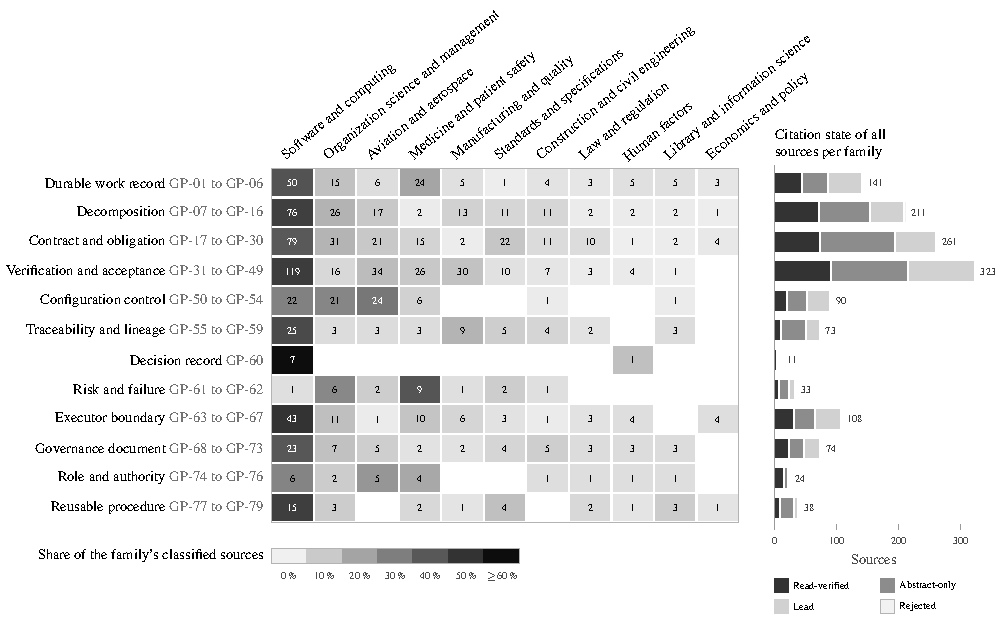
\includegraphics[width=\textwidth]{figures/f11/f11-literature-domains.pdf}
\caption{Located literature per mechanism family, by source domain and by citation state. On the left, each number counts the family's sources in one domain, and the shade gives that count as a share of the family's classified sources. The left panel does not show unclassified sources, and an empty cell is a zero count. On the right, each bar splits all sources of the family by citation state, with the total at its end. The counting rules are those of Table~\ref{tab:family-sources}: a source found for two families counts in both rows, and control items are excluded. Search agents assigned the domains and the citation states, and no human verification is recorded.}
\label{fig:family-domains}
\end{figure}

\begin{multicols}{2}
\subsection{Search procedure and limits}

The first search worked outward from mechanism families, since several patterns can share one research base. A later audit used a protocol fixed before that pass and searched all 79 patterns and the control items again. It recorded the queries, sources, and citation states. Deduplication matched source identifiers and titles, with conflicting matches or states recorded for review.

Only sources marked Read-verified could support result claims. Abstract-only sources could establish a work's existence and topic. Unchecked leads could support no substantive citation. Human checking against a primary record remained a separate requirement before bibliography acceptance.

The first pass had no registered protocol or fixed query set. The later audit agents used one general search engine to reach publisher pages, preprint archives, and institutional records. They could not query the separate discovery services named in the protocol directly. The source set therefore depends on that search engine's retrieval.

The audit allowed eight discovery queries per item. Twelve calls across nine items exceeded that limit, with reasons recorded. Sources found only through those calls were excluded from the result files. The planned re-search of 39 merged candidates and blind re-classification of 101 screening rejects were not completed.

\subsection{Agreement between repeated searches}

Duplicate dispatch produced paired searches for \hyperlink{gp-61}{GP-61} through \hyperlink{gp-69}{GP-69} under the same model, protocol, and date. Source matching used DOI, then arXiv identifier, then normalized title. Across 18 directed comparisons, 19 of 120 opened sources were found in the paired run, or 15.8 per cent.

This is observed identifier-based overlap, not a recall estimate for the literature. Different identifiers can hide a match: one recorded work appeared with a DOI in one run and as an unidentified lead in the other. These paired runs show that the retrieved source list was not stable. The map records what the searches found, not the limits of the available literature.

\subsection{The withdrawn rating instrument}

The method for rating literature support was withdrawn after its controls failed to separate relevant evidence from analogy reliably; the paper retains source attribution without support scores.

The source counts in Table~\ref{tab:family-sources} describe what the searches found. They do not measure how strongly the literature supports a pattern or how completely the searches cover a field.
\end{multicols}

\clearpage
\section{The Framework and Its Core Documents}
\label{app:framework}

\begin{multicols}{2}
The Framework for Keeping Complex Work Coherent Across Time is a system of principles, normative requirements, domain bindings, guidance, and checks for complex engineering work. The current release has five parts.

\begin{itemize}\setlength{\itemsep}{0pt}\setlength{\parskip}{0pt}
\item \textbf{Governing Principles}: the principles that define the governing model. Appendix~\ref{app:principles} reproduces them.
\item \textbf{Normative Structural Specification}: the mandatory project architecture that puts the Governing Principles into practice. Appendix~\ref{app:spec} reproduces it.
\item \textbf{Domain Profiles}: bindings of the abstract information model to concrete artifacts, locations, formats, and tools. The current reference bindings are the software profile and a hardware profile for physical systems. Appendix~\ref{app:entities} gives the software reference layout and the hardware differences.
\item \textbf{Guides}: explanatory and adoption material that helps people apply the framework. A guide adds no normative requirement and overrides none.
\item \textbf{Normative Checks}: deterministic checks that enforce the mechanically verifiable requirements of the Specification. The Specification states them in its \hyperlink{nss-16}{\S16}, and Appendix~\ref{app:checks} lists the minimum set.
\end{itemize}

The Governing Principles and the Specification are the domain-general core. The Domain Profiles, the Guides, and the Normative Checks support the use of that core. They do not override it.
\end{multicols}

The two core documents follow as issued, at version~1.0. The SHA-256 digest of each source file identifies the exact text reproduced here:

\begin{itemize}\setlength{\itemsep}{0pt}\setlength{\parskip}{0pt}
\item Governing Principles: {\footnotesize\texttt{76d4f0ed447fe1f4025446b66af0b662ef13b851b266162197ad06427fed9fa7}}
\item Normative Structural Specification: {\footnotesize\texttt{35345a1e802b127e64740b2a15dcd873fb315b5cada882b4dacef0fc709a9f59}}
\end{itemize}

\subsection{Governing Principles}
\label{app:principles}

\begin{multicols}{2}

\noindent{\large\bfseries Governing Principles for Complex Engineering Projects}\par\medskip

Author: Franz Bruckhoff

\hypertarget{gp-COD}{}

\subsubsection*{Component-Oriented Decomposition}

AI Agents working on complex long-horizon projects require stable, bounded units of work with explicit Contracts. They get that through Hierarchical Component Specifications, and not through flat lists of features or a monolithic requirements document.

This holds for software Systems, physical megastructures such as floating cities, energy Systems, transportation networks, or any other engineered System of high complexity.

Large Systems that stay coherent over time are decomposed into pieces with clear responsibilities, interfaces, and ownership boundaries. Those pieces are Components, such as modules, services, Subsystems, libraries, AI Agents, and layers. Without that decomposition the System becomes a monolith that no human team and no set of AI Agents can reason about, divide into parallel work, or change without constant global coordination.

It's therefore essential to prefer Components that can be replaced, upgraded, or removed with limited disruption to the rest of the System. Clean interfaces and explicit Contracts make this practical. Both humans and AI Agents benefit when a Component can be swapped without forcing redesign of high-stability elements.

Feature-centric thinking works only while the System is still small and mostly user-facing. Once the majority of the work is internal infrastructure, coordination logic, reliability mechanisms, or performance-critical paths, "features" become a forced and misleading frame. In software Systems that have end users, there are obviously user-facing Capabilities. In a floating city there are residential modules, power generation, desalination, docking systems, emergency response, governance interfaces, and so on. Some of those Capabilities are commonly called "features".

But the word "feature" has certain implications as a unit of work and specification:

\begin{itemize}\setlength{\itemsep}{0pt}\setlength{\parskip}{0pt}

\item It carries the assumption that the primary consumer is an end user and that the right framing is a user story.

\item Thinking in terms of "features" works cleanly only while the System is still small and mostly surface-level.

\item Once the majority of the effort is internal (coordination, reliability, interfaces between Subsystems, performance under load, safety Constraints, long-term maintainability, etc), forcing everything into "features" becomes artificial and misleading.

\end{itemize}

A floating city’s power distribution network, structural integrity monitoring, or waste-processing loops are not usefully described as features with user stories. They are Components with required behaviors, interfaces, Constraints, and Acceptance Criteria. The same is true for the majority of the work inside any ambitious software System after the first few user-visible slices.

So how do we go about features then?

\begin{itemize}\setlength{\itemsep}{0pt}\setlength{\parskip}{0pt}

\item A user-facing Capability is either its own Component or a required behavior of a larger Component.

\item When it's truly end-user facing, you may include one or a few short "user story" statements inside the Rationale section of the Component's Specification, which helps explain why the Component exists from the user's perspective.

\end{itemize}

In some rare edge cases like pure dataflow Systems the primary mental model starts with flows or roles rather than static Components. But even then those Systems end up being implemented as Components with defined interfaces.

There are some scenarios where the Component lens becomes secondary and impractical:

\begin{itemize}\setlength{\itemsep}{0pt}\setlength{\parskip}{0pt}

\item If you work on pure open-ended scientific exploration with no engineering deliverable or target artifact.

\item Certain forms of pure mathematical or theoretical work producing a single unified proof or insight rather than a constructed System.

\item Small-scale artistic or expressive works where modularity would actively harm the intended holistic quality.

\item Extremely short-lived, single-person prototypes where the overhead of formal decomposition exceeds any benefit (you already know that those days are counted).

\end{itemize}

But even in those scenarios, some form of decomposition emerges once the work grows beyond a certain size.

Therefore it is correct to treat Component-oriented decomposition as the default mental model.

\hypertarget{gp-LSA}{}

\subsubsection*{Layered System Architecture}

AI Agents working on complex long-horizon projects need a stable source of truth. They operate by reading Specifications, code, and Designs, then proposing or making changes. When essential purpose and critical Constraints are entangled with volatile implementation details, AI Agents must continually re-infer what must remain true. This increases inconsistency and error.

Stable, high-value parts of the System must not depend on volatile implementation details.

The essential purpose, Invariants (conditions or properties that must always remain true for the System, regardless of its state), and critical behaviors are treated as high-stability elements. These define what the System is and what it must guarantee.

The particular ways those guarantees are achieved (choice of technologies, materials, vendors, control systems, construction methods, interfaces, delivery mechanisms, configuration values, operating parameters, etc.) are treated as lower-stability elements.

Configuration values and parameters that belong to lower-stability elements should be kept explicit and external rather than buried inside high-stability design or logic.

Dependencies must flow from lower-stability elements toward higher-stability elements. High-stability elements must never depend on lower-stability elements.

Consequences:

\begin{itemize}\setlength{\itemsep}{0pt}\setlength{\parskip}{0pt}

\item AI Agents and humans can reason about, verify, and evolve the essential purpose and Invariants without being entangled in particular implementation choices.

\item Changes to materials, vendors, software frameworks, sensors, or construction techniques do not force redesign of what the System must guarantee.

\item The Blast Radius of AI Agent actions is limited: AI Agents may freely modify lower-stability elements without silently breaking the high-stability core.

\item High-stability elements can carry strong, relatively unchanging Acceptance Criteria that AI Agents or verification processes can check independently of current Realization details.

\item Multiple AI Agents can work on different lower-stability parts in parallel while sharing a common, stable Contract.

\item Over long-horizon projects, the core remains authoritative even as implementation technologies and methods are replaced repeatedly.

\end{itemize}

This principle applies equally to software Systems and to physical Systems like floating cities.

In software, high-stability elements include core domain rules, business Invariants, and critical System behaviors. Lower-stability elements include particular databases, web frameworks, UI libraries, cloud providers, or third-party services.

In a floating city, high-stability elements include structural integrity under marine conditions, life-support balance, safety Invariants, and long-term habitability. Lower-stability elements include specific hull materials, power-generation hardware, sensor models, or construction sequences.

\hypertarget{gp-IMF}{}

\subsubsection*{Integrated Modularity First}

For complex, long-horizon Systems, prefer a coherent design with strong internal Component boundaries over early hard separation.

A coherent design means the System has a clear overall purpose and fits together logically. Its parts work toward the same goals without conflicting or creating unnecessary complexity.

Establish clear Components and interfaces from the beginning. Keep the System as integrated as practical so that humans and AI Agents can reason about it, verify it, and evolve it with manageable coordination cost. Introduce hard separation only when the benefits clearly outweigh the added coordination and interface costs. Hard separation includes independent ownership, strong operational or physical isolation, independent fabrication, or independent evolution.

Valid reasons for hard separation include:

\begin{itemize}\setlength{\itemsep}{0pt}\setlength{\parskip}{0pt}

\item Different parts must evolve, be fabricated, or be operated at significantly different rates or under different constraints

\item Failure isolation is required so that problems in one part cannot cascade

\item Regulatory, safety, security, or ownership boundaries demand isolation

\item Geographic, environmental, or latency constraints force physical separation

\end{itemize}

Premature hard separation increases interface complexity, coordination overhead, and verification difficulty. Start with strong modularity inside a coherent System. Separate only when the need is concrete and the trade-offs are understood.

In software, this means starting with a modular monolith (one coherent codebase with clear internal Components) rather than jumping early to microservices. Split into separate services only when independent scaling, deployment, or failure isolation becomes a real requirement.

For a floating city, this means designing the overall structure, power, life support, and modules as an integrated System with clear interfaces, rather than treating every major Subsystem as fully independent from the start. Some strong physical separations (such as watertight compartments and fire zones) are required early for safety. Beyond those necessary isolations, introduce further hard separation only when safety, environmental, or functional constraints demand it.

\hypertarget{gp-VFE}{}

\subsubsection*{Verification-First Engineering}

No unit of work is done until it has been verified against explicit Acceptance Criteria and corrected until those criteria are met. Every meaningful artifact must have checkable criteria before it is accepted.

The required loop is:

\begin{enumerate}\setlength{\itemsep}{0pt}\setlength{\parskip}{0pt}

\item Draft against a stated set of Acceptance Criteria or Constraints.

\item Verify the draft against those criteria.

\item Identify specific defects (not vague dissatisfaction).

\item Correct only the identified defects. If the criteria themselves are incomplete or incorrect, the human must revise them; AI Agents may not alter Acceptance Criteria.

\item Re-verify. Accept and freeze the result only when the criteria are satisfied.

\end{enumerate}

Human acceptance is mandatory for high-stability, high-blast-radius, or high-stakes artifacts (core Invariants, major Component Specifications, safety-critical Designs, significant architectural decisions, and anything that defines System-level "done"). Lower-level work that sits inside already-accepted Contracts and criteria may be accepted by automated checks or by AI Agents operating strictly within those pre-approved bounds. The depth of verification must match the Blast Radius and stability of the artifact.

AI Agents may generate verification evidence and perform checks. They may not change the Acceptance Criteria.

Consequences:

\begin{itemize}\setlength{\itemsep}{0pt}\setlength{\parskip}{0pt}

\item Drift and silent quality loss are reduced because every change is checked against a fixed reference.

\item AI Agents receive clear, local signals about what is wrong instead of global or ambiguous feedback.

\item Rework stays bounded; corrections target concrete failures rather than restarting from scratch.

\item Long-horizon coherence is protected because accepted artifacts remain stable until a new, justified change is required.

\item Human attention stays on the decisions that only a human may make.

\end{itemize}

The principle is domain-general. In software it governs code, tests, and specifications. In a floating city it governs design documents, calculations, safety cases, and fabrication specifications. The form of the evidence differs between domains, but in every domain work is incomplete until it is verified.

An artifact that has not passed this loop is not done.

\hypertarget{gp-SaC}{}

\subsubsection*{Specifications as Contracts}

Specifications that define required behaviors, interfaces, or Acceptance Criteria are Contracts, not suggestions.

These Contracts state what must be true and what "done" means. Humans and AI Agents implement against them. They do not reinterpret, expand, or weaken them without explicit human authority.

Changing a Contract requires human decision. AI Agents may propose revisions; they may not enact them. Once accepted, a Contract remains the authoritative reference until the human revises it.

Consequences:

\begin{itemize}\setlength{\itemsep}{0pt}\setlength{\parskip}{0pt}

\item Work has a fixed target instead of open-ended interpretation.

\item Implementation drift is constrained.

\item Verification has a stable reference.

\item Humans keep control of purpose, scope, and the definition of "done".

\end{itemize}

This applies to any engineered System. The documents may be Component Specifications, interface definitions, design specifications, or safety requirements. In each case, the document is a Contract.

A Specification treated as optional guidance is not a Contract and does not satisfy this principle.

\subsubsection*{Normative Structural Specification}

The Normative Structural Specification is written in full in Normative Structural Specification. That file is the authoritative structural document of the Framework for Keeping Complex Work Coherent Across Time.

The Specification defines the required project artifacts (VISION, Governing Principles, the Component Specification Graph, Interface Declarations, Decision Records, Verification Artifacts, Baselines, Registers, and the Work Record) together with their layout, their content rules, and the deterministic checks that enforce them. It operationalizes the five principles above: every clause is traceable to one or more of the 79 Adopted structural forms in research/project-structure-patterns/Generalized Patterns.md or to a frozen principle.

In any conflict over project structure, the Normative Structural Specification governs.

\end{multicols}

\clearpage
\subsection{Normative Structural Specification}
\label{app:spec}

\begin{multicols}{2}

\noindent{\large\bfseries Normative Structural Specification for Complex Engineering Projects}\par\medskip

Author: Franz Bruckhoff

This is the structural document of the Framework for Keeping Complex Work Coherent Across Time. It states what an adopting Project must contain, how the elements relate, and which rules bind them. Where each element lives is declared by each Project's Path Map, not by this Specification (\hyperlink{nss-1.8}{\S1.8}, \hyperlink{nss-14.8}{\S14.8}). It operationalizes the five core principles of Governing Principles: Component-Oriented Decomposition (\hyperlink{gp-COD}{COD}), Layered System Architecture (\hyperlink{gp-LSA}{LSA}), Integrated Modularity First (\hyperlink{gp-IMF}{IMF}), Verification-First Engineering (\hyperlink{gp-VFE}{VFE}), and Specifications as Contracts (\hyperlink{gp-SaC}{SaC}).

Every normative clause is traceable to one or more of the 79 Adopted structural forms (\hyperlink{gp-01}{GP-01} to \hyperlink{gp-79}{GP-79}) in Generalized Patterns or to a frozen principle. Each clause ends with a traceability bracket naming its grounds. \hyperlink{nss-appB}{Appendix B} gives the complete mapping. Where this Specification and any other framework document conflict on structure, this Specification governs.

\textbf{Scope of application}

This Specification defines the structural foundation for Projects that adopt the Framework for Keeping Complex Work Coherent Across Time. Its clauses bind an adopting Project, and a deviation is allowed only as recorded in the Deviation Matrix (\hyperlink{nss-1.5}{\S1.5}, \hyperlink{nss-9.4}{\S9.4}). Not every clause is equally relevant to every Project. The core sections apply to all adopting Projects. The depth and formality with which each required artifact is produced scale with the Criticality Class of the Component or Capability it governs and with the overall risk and complexity of the Project, as defined in \hyperlink{nss-1.6}{\S1.6} and \hyperlink{nss-7.10}{\S7.10}.

\hypertarget{nss-1}{}

\subsubsection*{1 Purpose, Scope, and Compliance}

\hypertarget{nss-1.1}{}

\par\smallskip\noindent\textbf{1.1 Authority}\par\nopagebreak

This Specification defines the required structure of every Project built under the Framework for Keeping Complex Work Coherent Across Time: the required artifacts, their content rules, their directional relationships, and the Normative Checks that enforce them. It is the structural reference for humans and AI Agents alike. Concrete storage of the artifacts is declared by each Project's Path Map (\hyperlink{nss-1.8}{\S1.8}, \hyperlink{nss-14.8}{\S14.8}). [Goal \hyperlink{nss-6.2}{\S6.2}; \hyperlink{gp-SaC}{SaC}]

\hypertarget{nss-1.2}{}

\par\smallskip\noindent\textbf{1.2 Domain of application}\par\nopagebreak

This Specification is intended to support engineered Systems of high complexity across domains, including software platforms, robotic Systems, and floating cities. Its core clauses avoid domain-specific assumptions. Domain practice adds the methods and controls required by each field, with any structural deviation recorded under \hyperlink{nss-1.5}{\S1.5}. [Goal P3; \hyperlink{gp-16}{GP-16}]

\hypertarget{nss-1.3}{}

\par\smallskip\noindent\textbf{1.3 Human authority}\par\nopagebreak

Purpose, Invariants, risk acceptance, and the definition of done belong to the human owner. AI Agents may draft, propose, and implement; they may not enact changes to purpose, Contracts, Acceptance Criteria, or risk acceptance. Every clause of this Specification preserves this division. [Goal P4; Goal \hyperlink{nss-5}{\S5}; \hyperlink{gp-VFE}{VFE}; \hyperlink{gp-SaC}{SaC}]

\hypertarget{nss-1.4}{}

\par\smallskip\noindent\textbf{1.4 Completeness of structure}\par\nopagebreak

The Project structure must cover four recursive process groups at every level of the System:

\begin{enumerate}\setlength{\itemsep}{0pt}\setlength{\parskip}{0pt}

\item \textbf{Agreement}: formal commitments with external parties (customers, users, partners, regulators, vendors, contractors, etc.).

\item \textbf{Project-enabling}: the supporting work that makes the Project possible (tooling, configuration, quality infrastructure, shared services, etc.).

\item \textbf{Technical management}: planning, monitoring, decision-making, risk handling, control of the work, etc.

\item \textbf{Technical}: the actual engineering work (defining, designing, realizing, verifying, etc.) of the System.

\end{enumerate}

These groups classify required coverage. They do not prescribe any particular life-cycle model. No level of the System may omit the agreement processes or the verification processes. [\hyperlink{gp-16}{GP-16}]

\hypertarget{nss-1.5}{}

\par\smallskip\noindent\textbf{1.5 Compliance and deviation}\par\nopagebreak

Every clause of this Specification is binding. A deviation is allowed only when it is recorded as an explicit entry in the Deviation Matrix (\hyperlink{nss-9.4}{\S9.4}). Each entry must name:

\begin{itemize}\setlength{\itemsep}{0pt}\setlength{\parskip}{0pt}

\item what is being waived,

\item why the waiver is needed, and

\item which named human accepted the risk.

\end{itemize}

The matrix starts empty. Most Projects will have few or no entries. Implicit or unspoken deviation is prohibited. The purpose of this rule is transparency and human accountability, not bureaucracy. [\hyperlink{gp-53}{GP-53}; \hyperlink{gp-SaC}{SaC}]

\hypertarget{nss-1.6}{}

\par\smallskip\noindent\textbf{1.6 Formality scales with risk; every required Entity must exist}\par\nopagebreak

No Entity required by this Specification may be omitted; only the depth of its instances may be adjusted.

The amount of detail, documentation, and review applied to each artifact scales with two factors:

\begin{itemize}\setlength{\itemsep}{0pt}\setlength{\parskip}{0pt}

\item the Criticality Class of the Component or Capability it governs (see \hyperlink{nss-7.10}{\S7.10}), and

\item the overall risk and complexity of the Project.

\end{itemize}

Low-criticality work may use lightweight versions of the required artifacts. High-criticality or safety-relevant work must use fuller, more rigorous versions. The decision to use a lighter or fuller version must be recorded with a short rationale in the Criticality Record (\hyperlink{nss-7.10}{\S7.10}).

This clause governs the depth of a required artifact only; it does not override \hyperlink{nss-1.5}{\S1.5}. Omission of a required Entity remains possible solely as an entry in the Deviation Matrix (\hyperlink{nss-9.4}{\S9.4}). [\hyperlink{gp-39}{GP-39}; \hyperlink{gp-VFE}{VFE}]

\hypertarget{nss-1.7}{}

\par\smallskip\noindent\textbf{1.7 This Specification is high-stability}\par\nopagebreak

Individual Projects must not create their own versions of this Specification. If a Project needs to deviate from any clause, it must do so explicitly using the deviation process in \hyperlink{nss-1.5}{\S1.5}.

The Specification may be changed only by a human decision recorded as a Decision Record (\hyperlink{nss-11}{\S11}) that states the reason for the change and its consequences. [\hyperlink{gp-LSA}{LSA}; \hyperlink{gp-SaC}{SaC}]

\hypertarget{nss-1.8}{}

\par\smallskip\noindent\textbf{1.8 Abstract information model, concrete storage}\par\nopagebreak

This Specification defines an abstract information architecture: the required Entities, their required content, their directional relationships, and the Gates that bind them. It does not prescribe concrete storage. Filesystem paths, directory trees, file names, and serialization formats (Markdown, YAML, JSON, domain-native model formats, etc.) are declared by each Project in its Path Map (\hyperlink{nss-14.8}{\S14.8}).

This separation is deliberate, for four reasons:

\begin{itemize}\setlength{\itemsep}{0pt}\setlength{\parskip}{0pt}

\item \textbf{No ontological mismatch.} A standard defines requirements and an information model. Hardcoded storage paths would conflate the meta-model of the architecture with one storage implementation of it.

\item \textbf{Domain-native tooling.} Domains work in different native formats: declarative interface schemas, structured data files, parametric models, tabular mass-property data, etc. Forcing one serialization on every domain creates friction between the System description and the tools that produce and check it.

\item \textbf{Checkable serialization.} Human-readable prose formats are fragile for the automated parsing of relational data (dependency graphs, ledger entries, Obligation matrices, etc.). The serialization format of each Entity is therefore a declared Project choice, so that Normative Checks can parse each Entity in a format suited to mechanical verification.

\item \textbf{Composability.} A concrete layout that serves one domain well can be reused by other Projects in that domain. Ready-made layout guides for particular domains may exist outside this Specification. They are not part of it and bind nothing: a Project's Path Map governs, whatever its bindings were modelled on.

\end{itemize}

[Goal DR1; Goal P3; \hyperlink{gp-LSA}{LSA}]

\hypertarget{nss-2}{}

\subsubsection*{2 Terminology}

The terms below are defined once and used consistently throughout this Specification.

\begin{itemize}\setlength{\itemsep}{0pt}\setlength{\parskip}{0pt}

\item \textbf{Acceptance Criteria}: the checkable statements that define "done" for a unit.

\item \textbf{AI Agent}: an Executor that is an AI system rather than a human.

\item \textbf{Baseline}: an approved, frozen snapshot of the description of the System or of its Realization, at a defined level.

\item \textbf{Baseline Ledger}: the register that records every approved Baseline: the artifacts it governs, its snapshot identifier, its status, and the named human who accepted the lock (\hyperlink{nss-9.1}{\S9.1}).

\item \textbf{Blast Radius}: the set of System elements that a given change or failure can affect.

\item \textbf{Capability}: a function the System delivers to its users or operators. A Capability may span several Components.

\item \textbf{Component}: a bounded unit of responsibility with explicit interfaces, Contracts, and Acceptance Criteria.

\item \textbf{Component Specification}: the normative document that defines one Component (Rationale, Required Behaviors, Acceptance Criteria, Constraints, Dependencies \& Interfaces, plus its private Design).

\item \textbf{Constraint}: an Obligation that limits how a need may be met rather than stating what must be achieved.

\item \textbf{Contract}: the human-approved part of a Specification that other Components may rely on. It primarily contains the Obligations, interfaces, Invariants, and Acceptance Criteria.

\item \textbf{Criticality Class}: the recorded class assigned to a Component or a Capability that determines the Obligations and the verification rigor applying to it.

\item \textbf{Criticality Record}: the register that holds the Criticality Class assigned to each Component and Capability, together with the tailoring decisions and rationales that other clauses direct into it (\hyperlink{nss-7.10}{\S7.10}).

\item \textbf{Decision Record}: a numbered, immutable record of one binding decision.

\item \textbf{Design}: how a Component satisfies its Contract. Visible only to the Component’s implementer; binds no other Component.

\item \textbf{Deviation Matrix}: the register that records every deviation from this Specification, naming what is waived, why, and which named human accepted the risk (\hyperlink{nss-9.4}{\S9.4}).

\item \textbf{Entity}: a class of element required by this Specification, of which a Project holds one or more instances. \hyperlink{nss-appA}{Appendix A} lists every required Entity; the Path Map (\hyperlink{nss-14.8}{\S14.8}) binds each Entity to concrete storage.

\item \textbf{Entry Point}: the single short document that serves as the starting map of the Project Record. Every Executor begins here and is directed from it to the deeper artifacts relevant to their work. It declares the Path Map that binds every required Entity to its concrete location (\hyperlink{nss-14.3}{\S14.3}, \hyperlink{nss-14.8}{\S14.8}).

\item \textbf{Exploratory Work Unit}: a bounded, time- or resource-capped Work Unit executed in an isolated workspace to investigate candidate questions (feasibility, empirical models, candidate Specifications, etc.). Its completion is defined by meeting declared stopping criteria and producing structured findings recorded in the Project Record, not by modifying the canonical Realization or System description.

\item \textbf{Executor}: a human or an AI system performing work under a bounded mandate.

\item \textbf{Gate}: a controlled passage between Phases, closed only by a human decision recorded as a Decision Record (\hyperlink{nss-11}{\S11}).

\item \textbf{Governance Document}: a human-authored standing directive (principles, rules, instructions, etc.) addressed to Executors.

\item \textbf{Invariant}: a property that must always hold and that no Executor may weaken without human authorization.

\item \textbf{Key Design Parameter}: one of a small named set of parameters that govern System success.

\item \textbf{Normative Check}: a mechanically executable rule that verifies whether Project artifacts comply with a structural requirement of this Specification.

\item \textbf{Obligation}: one verifiable requirement statement.

\item \textbf{Operational Concept}: the statement of how the System will be operated and sustained.

\item \textbf{Path Map}: the deterministic declaration, held in the Entry Point, that binds every required Entity of this Specification to a concrete location pattern and a serialization format (\hyperlink{nss-14.8}{\S14.8}).

\item \textbf{Phase}: a bounded stage of work that produces at least one durable artifact and is entered and left through a Gate.

\item \textbf{Plan Document}: the binding document that governs one Work Unit, stating its scope, its Acceptance Criteria, its progress, and the decisions taken under it. It is the artifact an Executor follows in preference to any conversational instruction.

\item \textbf{Production Work Unit}: a Work Unit that modifies the canonical Realization or System description under an approved Specification and an approved Plan Document.

\item \textbf{Project}: the bounded endeavor that produces and sustains one System, governed by one Project Record.

\item \textbf{Project Record}: the versioned set of durable artifacts that constitutes the system of record for the Project.

\item \textbf{Realization}: the actual built System or Component, as distinct from its description.

\item \textbf{Reference Realization}: a maintained instance that embodies the current interpretation of a Contract, against which the governed element is compared to detect drift (\hyperlink{nss-7.17}{\S7.17}). Distinct from a Verification Reference State.

\item \textbf{Registry}: the machine-readable index of every Component and content item in the System.

\item \textbf{Risk Register}: the register that records every identified risk with its owner, analysis, mitigation plan, tracking method, and closure (\hyperlink{nss-12.1}{\S12.1}).

\item \textbf{Specification}: the normative description of a Component or an effort. It consists of the Contract plus the Design.

\item \textbf{Stability Class}: the classification of an element by expected rate of change. Dependencies must point only toward elements of equal or higher Stability Class.

\item \textbf{Status Ledger}: the register that records the status and history of every change, deviation, waiver, and audit outcome (\hyperlink{nss-9.3}{\S9.3}).

\item \textbf{Subsystem}: a Component that is also a System at a lower level of decomposition. It contains interacting Components and must satisfy the Contract of its containing System.

\item \textbf{System}: the engineered artifact under construction, in any domain.

\item \textbf{Verification Artifact}: the durable record that an Acceptance Criterion was checked, including the outcome.

\item \textbf{Verification Plan}: the governing document that fixes the scope, responsibilities, resources, and completion criteria of verification for the Project.

\item \textbf{Verification Procedure}: a concrete procedure that can be executed to determine whether one or more Acceptance Criteria are satisfied. The durable record of running a Verification Procedure is a Verification Artifact.

\item \textbf{Verification Reference State}: the recorded outcome of executing whatever verification exists immediately before a change begins, used as the comparison point for that change. Distinct from a Baseline (\hyperlink{nss-9.1}{\S9.1}).

\item \textbf{Vision Document}: the human-authored statement of the System's purpose, problem, desired future state, and long-term goals.

\item \textbf{Work Record}: the single structured, queryable artifact that records every Work Unit, any typed relations between Work Units, and the discoveries made during their execution.

\item \textbf{Work Unit}: a bounded unit of work with declared scope, an assigned Executor, and Acceptance Criteria.

\end{itemize}

\hypertarget{nss-3}{}

\subsubsection*{3 Purpose}

\hypertarget{nss-3.1}{}

\par\smallskip\noindent\textbf{3.1 One Vision Document}\par\nopagebreak

Every Project must have exactly one Vision Document. It states the essential problem being solved, the concrete desired future state, and the long-term goals that define success. It is short, stable, free of implementation detail, and written so that the gap between current reality and the desired outcome is clear, credible, and memorable after a single reading. It is the first artifact created and is human-authored. [\hyperlink{gp-13}{GP-13}; \hyperlink{gp-68}{GP-68}; \hyperlink{gp-LSA}{LSA}]

\hypertarget{nss-3.2}{}

\par\smallskip\noindent\textbf{3.2 Highest stability}\par\nopagebreak

The Vision Document is the highest-stability artifact of the Project. It must change only rarely, and only through the controlled change Gate (\hyperlink{nss-9.2}{\S9.2}) and a Decision Record (\hyperlink{nss-11}{\S11}).

No implementation choices, technology selections, material choices, vendor names, or detailed design decisions, etc. may appear in the Vision Document. Those details belong in lower-stability documents. [\hyperlink{gp-50}{GP-50}; \hyperlink{gp-51}{GP-51}; \hyperlink{gp-LSA}{LSA}]

\hypertarget{nss-3.3}{}

\par\smallskip\noindent\textbf{3.3 Hierarchy of intent}\par\nopagebreak

The Vision Document sits at the top of the hierarchy. Every lower-level document that states or plans work (Component Specifications, Plan Documents, design documents, etc.) must explain how it serves the goals stated in the Vision Document. No lower-level document may change, contradict, or redefine the problem, desired future state, or long-term goals that the Vision Document has already accepted. [\hyperlink{gp-13}{GP-13}]

\hypertarget{nss-4}{}

\subsubsection*{4 The Project Record}

\hypertarget{nss-4.1}{}

\par\smallskip\noindent\textbf{4.1 Sole system of record}\par\nopagebreak

All state that governs work must exist as durable, versioned, human-readable artifacts inside the Project Record. This includes Plan Documents, progress, decisions, open issues, and verification outcomes. Agreements held only outside the Project Record (in conversation, message channels, Executor memory, etc.) have no governing force and must be written into the Project Record before they become binding. Completed Plan Documents must remain in the record as history. The depth and formality of these artifacts may scale with Project criticality, but their existence is required. [\hyperlink{gp-01}{GP-01}; \hyperlink{gp-06}{GP-06}]

\hypertarget{nss-4.2}{}

\par\smallskip\noindent\textbf{4.2 Durable work, disposable Executor instances}\par\nopagebreak

Executor instances are disposable; the work product is durable. All meaningful work product must exist as versioned artifacts in the Project Record. Shared decisions must be recorded append-only and must be read by every Executor before work where relevant. Progress must accumulate only in the Project Record, never solely in the memory or private context of an Executor. [\hyperlink{gp-65}{GP-65}; \hyperlink{gp-01}{GP-01}; \hyperlink{gp-02}{GP-02}]

\hypertarget{nss-4.3}{}

\par\smallskip\noindent\textbf{4.3 One canonical source per concern}\par\nopagebreak

For every concern, exactly one artifact is the canonical source of truth. The Project must declare, in a single place readable by every Executor, which artifact governs each concern and how those artifacts relate to one another. Any derived artifact (indexes, ledgers, summaries, compliance records, etc.) must be generated from its canonical source and must never be maintained in parallel with it. Conflicting sources for one concern are a defect and must be resolved by designating one source and demoting the others. [\hyperlink{gp-59}{GP-59}]

\hypertarget{nss-4.4}{}

\par\smallskip\noindent\textbf{4.4 Machine-readable, checkable surfaces}\par\nopagebreak

Every surface of the System on which an Executor is expected to act (documents, interfaces, structured records, declared instructions, etc.) must be machine-readable and checkable. The human owner must own the Contract and the top-level decomposition; Executors implement beneath. [\hyperlink{gp-76}{GP-76}]

\hypertarget{nss-4.5}{}

\par\smallskip\noindent\textbf{4.5 Work Record}\par\nopagebreak

Every Project must maintain one Work Record: a structured, queryable artifact kept under the same version control as the System description, capturing every Work Unit and the discoveries made during execution. Unstructured prose lists must not serve as the system of record. Where Work Units carry dependencies, those dependencies must be recorded as typed relations (at minimum: blocks, part-of, supersedes, etc.); a Work Unit is then eligible for execution only when every relation that blocks it is resolved, and completing a unit must release its dependents. [\hyperlink{gp-04}{GP-04}; \hyperlink{gp-05}{GP-05}]

\hypertarget{nss-4.6}{}

\par\smallskip\noindent\textbf{4.6 One binding Plan Document per Work Unit}\par\nopagebreak

Each Work Unit must be governed by one binding Plan Document, which the Executor follows in preference to any conversational instruction. The unchecked Acceptance Criteria in the document constitute the queue of remaining work. A conflict between the Plan Document and an instruction must be resolved in favor of the Plan Document or escalated to the human owner. The Plan Document itself must record its current progress and the decisions taken under it. [\hyperlink{gp-03}{GP-03}; \hyperlink{gp-01}{GP-01}]

\hypertarget{nss-4.7}{}

\par\smallskip\noindent\textbf{4.7 Iteration discipline}\par\nopagebreak

Each work iteration must proceed as follows:

\begin{enumerate}\setlength{\itemsep}{0pt}\setlength{\parskip}{0pt}

\item Read the current state from the Project Record.

\item Complete exactly one Work Unit.

\item Verify that unit against its Acceptance Criteria.

\item Record the new state and the verification outcome before the next iteration begins.

\end{enumerate}

The size of the Work Unit is governed by the sizing and Blast Radius rules in \hyperlink{nss-5.5}{\S5.5} and \hyperlink{nss-5.6}{\S5.6}. [\hyperlink{gp-02}{GP-02}; \hyperlink{gp-VFE}{VFE}]

\hypertarget{nss-4.8}{}

\par\smallskip\noindent\textbf{4.8 Concurrent contributions merge through one role}\par\nopagebreak

Where more than one Executor contributes to the same shared artifact at the same time, their contributions must be prepared separately and merged into the canonical artifact by one named role. No Executor may write directly to a canonical artifact while a merge is pending. The named role may be a human or a declared process, and it must be recorded in the Project Record for the duration of the concurrent work. [\hyperlink{gp-65}{GP-65}]

\hypertarget{nss-4.9}{}

\par\smallskip\noindent\textbf{4.9 Governance Documents are controlled artifacts}\par\nopagebreak

Governance Documents (including reusable instructions given to AI Agents) must be versioned, reviewable, and checkable artifacts in the Project Record under direct human editing. Governance Document content hidden inside tools or frameworks is prohibited. [\hyperlink{gp-66}{GP-66}]

\hypertarget{nss-5}{}

\subsubsection*{5 Decomposition and Work Units}

\hypertarget{nss-5.1}{}

\par\smallskip\noindent\textbf{5.1 Deliverable-anchored decomposition}\par\nopagebreak

Project decomposition must be organized around the deliverables the Project produces, not around the Executors doing the work or around organizational structure. Every decomposition element must carry a short definition stating what the element is and what it delivers. The identity of an element must not depend on which Executor performs the work. Work that yields no deliverable (management, integration, etc.) must appear as explicit elements. [\hyperlink{gp-07}{GP-07}; \hyperlink{gp-COD}{COD}]

\hypertarget{nss-5.2}{}

\par\smallskip\noindent\textbf{5.2 Purpose-defined Components}\par\nopagebreak

The System must be decomposed into Components defined by the purpose they serve, not by physical form, packaging, or implementation technology, etc. Each Component must carry its own Obligations and design criteria, one named human owner, and a Verification Procedure that yields a binary pass/fail status readable by anyone. Obligations, ownership, and pass/fail status of any Component must be retrievable on demand. [\hyperlink{gp-08}{GP-08}; \hyperlink{gp-COD}{COD}]

\hypertarget{nss-5.3}{}

\par\smallskip\noindent\textbf{5.3 System level before Component detail}\par\nopagebreak

System-level interactions and cross-boundary Contracts must be defined before Component internals. Each Component must be designed against declared System behavior and the interfaces it declares with other Components. Where local and System-level optimization conflict, the System-level optimum governs. The local cost accepted for that System gain must be recorded as a Decision Record (\hyperlink{nss-11}{\S11}). A change that crosses a boundary must be agreed at System level before it is made inside a Component. [\hyperlink{gp-09}{GP-09}; \hyperlink{gp-COD}{COD}]

\hypertarget{nss-5.4}{}

\par\smallskip\noindent\textbf{5.4 Integrated modularity first}\par\nopagebreak

The default structure is one coherent System with strong internal Component boundaries. Hard separation (independent ownership, strong operational or physical isolation, independent fabrication, independent evolution, etc.) is introduced only when a concrete need exists (significantly different rates or constraints of evolution, required failure isolation, regulatory or safety boundaries, physical constraints, etc.) and its benefits clearly outweigh the added coordination and interface costs. Premature hard separation is a defect. [\hyperlink{gp-IMF}{IMF}]

\hypertarget{nss-5.5}{}

\par\smallskip\noindent\textbf{5.5 Sizing}\par\nopagebreak

Significant work that is assigned to an Executor must be decomposed into Work Units that one Executor can complete in one bounded effort while meeting the Work Unit’s Acceptance Criteria. An oversized Work Unit must be split before execution begins. AI Agents may propose the decomposition and the sizing. The human owner remains the final authority on any sizing decision that could affect higher-level Contracts, Invariants, or the definition of done. Work Units that stay strictly inside already-accepted higher-level Contracts and Acceptance Criteria may be sized by AI Agents. [\hyperlink{gp-10}{GP-10}]

\hypertarget{nss-5.6}{}

\par\smallskip\noindent\textbf{5.6 Work Units bounded by Blast Radius}\par\nopagebreak

Before a Work Unit starts, its Blast Radius must be estimated and bounded. Parallel Work Units must have non-overlapping Blast Radii. A change whose Blast Radius cannot be bounded must be decomposed further before execution. [\hyperlink{gp-12}{GP-12}]

\hypertarget{nss-5.7}{}

\par\smallskip\noindent\textbf{5.7 Work Units must be verifiable}\par\nopagebreak

Significant work assigned to an Executor must be packaged as a Work Unit: a bounded scope with checkable Acceptance Criteria. Work Units belong to one of two classes:

\begin{itemize}\setlength{\itemsep}{0pt}\setlength{\parskip}{0pt}

\item \textbf{Production Work Units}: modify the canonical Realization or System description. Each unit must execute in isolation, governed by a pre-existing Specification and a human-approved Plan Document (\hyperlink{nss-6.13}{\S6.13}). A Production Work Unit is complete only when its Verification Procedures pass.

\item \textbf{Exploratory Work Units}: investigate feasibility, test empirical models, optimize parameters, or discover candidate Specifications. Governed by explicit research questions, resource ceilings (time, token, compute budgets, etc.), and stopping criteria. An Executor operating under a human-approved exploratory mandate may spawn and iterate internal exploratory loops autonomously within declared resource boundaries.

\end{itemize}

Large efforts must be decomposed into bounded Work Units before execution begins. [\hyperlink{gp-11}{GP-11}; \hyperlink{gp-VFE}{VFE}]

\hypertarget{nss-5.8}{}

\par\smallskip\noindent\textbf{5.8 Nested levels of intent}\par\nopagebreak

Decomposition must form nested levels of intent: each level states why the work below it exists and is governed by Acceptance Criteria at its own level. Purpose belongs to the outermost level (the Vision Document, \hyperlink{nss-3.3}{\S3.3}). No inner level may redefine the Acceptance Criteria of a level above it. [\hyperlink{gp-13}{GP-13}]

\hypertarget{nss-5.9}{}

\par\smallskip\noindent\textbf{5.9 Work Units for long-horizon work}\par\nopagebreak

Long-horizon work must be decomposed into Work Units, each small enough for one Executor to complete and verify in one bounded effort. Each Work Unit must carry its own Acceptance Criteria and the Verification Procedures that confirm them. The Verification Procedures must run at the end of every Work Unit. Failures must be repaired before the next Work Unit starts. The governing Specification is frozen against drift; a change to it requires a Decision Record (\hyperlink{nss-11}{\S11}). [\hyperlink{gp-14}{GP-14}; \hyperlink{gp-VFE}{VFE}]

\hypertarget{nss-5.10}{}

\par\smallskip\noindent\textbf{5.10 Reusable task definitions}\par\nopagebreak

Recurring kinds of work must be defined once as reusable task-definition documents. In AI coding environments these are commonly called skills. In complex engineering and simulation environments they are more often called procedures or templates. Each document must contain:

\begin{itemize}\setlength{\itemsep}{0pt}\setlength{\parskip}{0pt}

\item an imperative sequence of steps

\item the Acceptance Criteria that must be satisfied when the work is done

\item the actions the Executor must not take

\item any required inputs (and their expected source)

\end{itemize}

Each document must also carry a short summary of when it applies, so an Executor can select the applicable task definition. Each task-definition document is a Governance Document (\hyperlink{nss-4.9}{\S4.9}). The name and terminology used may follow the conventions of the tools and domain in use; the binding to concrete storage is declared in the Path Map (\hyperlink{nss-14.8}{\S14.8}). [\hyperlink{gp-77}{GP-77}]

\hypertarget{nss-6}{}

\subsubsection*{6 Component Specifications and Contracts}

\hypertarget{nss-6.1}{}

\par\smallskip\noindent\textbf{6.1 Component Specifications}\par\nopagebreak

The Project must maintain a set of atomic Component Specifications: one Component Specification per Component, each a discrete, separately addressable artifact of the Project Record. Each Component Specification defines one coherent unit of responsibility. These are the primary documents that humans and AI Agents implement against. If a Component grows too large to keep its Required Behaviors and Acceptance Criteria consistent, it must be decomposed further. Component Specifications are written in System terms. User-story language is never the primary framing; it may appear only as optional context inside the Rationale section of a truly end-user-facing Component. [\hyperlink{gp-COD}{COD}; \hyperlink{gp-SaC}{SaC}]

\hypertarget{nss-6.2}{}

\par\smallskip\noindent\textbf{6.2 Required sections, linted}\par\nopagebreak

Every Component Specification must contain these sections, checked by Normative Checks (\hyperlink{nss-16}{\S16}):

\begin{itemize}\setlength{\itemsep}{0pt}\setlength{\parskip}{0pt}

\item \textbf{Rationale}: why this Component must exist. May contain one to a few short user-story statements if the Component is end-user facing.

\item \textbf{Required Behaviors}: precise description of what the Component must do, in System terms.

\item \textbf{Acceptance Criteria}: testable conditions that define "done".

\item \textbf{Constraints}: hard limits (performance, safety, resources, etc.).

\item \textbf{Dependencies \& Interfaces}: explicit declaration of relationships: the Components or interfaces this one requires; the interfaces or Contracts this one provides; and any containment ("part of") relationship.

\end{itemize}

[\hyperlink{gp-COD}{COD}; \hyperlink{gp-SaC}{SaC}; \hyperlink{gp-VFE}{VFE}]

\hypertarget{nss-6.3}{}

\par\smallskip\noindent\textbf{6.3 Public Contract, private Design}\par\nopagebreak

Each Component Specification splits into a public Contract and a private Design. The Contract comprises the five required sections listed in \hyperlink{nss-6.2}{\S6.2} and is visible to the Executors of every Component that has a declared interface or dependency relationship with it. The Design is visible only to the Executor(s) implementing that Component. Every other Component must rely on the Contract alone. An Executor working on a Component must receive that Component's full Specification and the Contracts of the Components with which it has declared interface or dependency relationships, not the whole System description. [\hyperlink{gp-27}{GP-27}]

\hypertarget{nss-6.4}{}

\par\smallskip\noindent\textbf{6.4 The Specification is the durable alignment artifact}\par\nopagebreak

The Realization is derived from and governed by the Specification. Where a Realization can be regenerated, it must be regenerated from the Specification rather than edited independently; where it cannot, the Specification remains the governing description and any divergence between the two is a defect in the Realization. Alignment, discussion, and versioning must occur at the Specification level. Specifications must be human-readable, versioned, maintained with a changelog, and open to contribution from any relevant discipline. [\hyperlink{gp-19}{GP-19}; \hyperlink{gp-SaC}{SaC}]

\hypertarget{nss-6.5}{}

\par\smallskip\noindent\textbf{6.5 Obligation statements}\par\nopagebreak

Obligations in Required Behaviors and Constraints must be expressed as unique, quantitative, verifiable statements. Each statement must name exactly one commitment in a fixed structure: the condition under which it holds, the subject that must act, the action, the object, and the constraint on the action. Ambiguous or compound statements must be rewritten until each statement is independently checkable. [\hyperlink{gp-20}{GP-20}; \hyperlink{gp-21}{GP-21}]

\hypertarget{nss-6.6}{}

\par\smallskip\noindent\textbf{6.6 Obligation attributes}\par\nopagebreak

Every Obligation must carry fixed attributes: identifier, owner, type, priority, source, rationale, status, and verification method. Obligations are organized in levels that mirror the decomposition: from the expectations of the parties the System serves (customers, users, regulators, etc.), through the Operational Concept (\hyperlink{nss-6.17}{\S6.17}), down to Component Obligations. The type of an Obligation (what it constrains) governs which verification method is admissible for it. Attribute rigor scales with Criticality Class (\hyperlink{nss-7.10}{\S7.10}). [\hyperlink{gp-22}{GP-22}; \hyperlink{gp-39}{GP-39}]

\hypertarget{nss-6.7}{}

\par\smallskip\noindent\textbf{6.7 Named owner for every Obligation}\par\nopagebreak

Every Obligation must be owned by one named human, never by a department or a role. The owner is the person who can be asked why the Obligation exists. An Obligation without a named human owner is not valid. [\hyperlink{gp-23}{GP-23}]

\hypertarget{nss-6.8}{}

\par\smallskip\noindent\textbf{6.8 Constraint provenance}\par\nopagebreak

Every Constraint must be marked as externally imposed (contract, regulation, physics, etc.) or internally owned. Externally imposed Constraints are fixed for the Project. Internally owned Constraints may be questioned and renegotiated through their named owner. [\hyperlink{gp-24}{GP-24}]

\hypertarget{nss-6.9}{}

\par\smallskip\noindent\textbf{6.9 Verification method assigned at authoring}\par\nopagebreak

The verification method for an Obligation must be assigned when the Obligation is authored, not after design is underway. An Obligation without a verification method must not enter a Baseline (\hyperlink{nss-9.1}{\S9.1}). Verification Procedures must run continuously as the design develops, not only at a late Gate. [\hyperlink{gp-25}{GP-25}; \hyperlink{gp-VFE}{VFE}]

\hypertarget{nss-6.10}{}

\par\smallskip\noindent\textbf{6.10 Interface declarations}\par\nopagebreak

Every interface between Components must be captured through one fixed lens that contains four elements: description, responsibility and change authority, reference frames with units and tolerances, and a checklist of the interaction categories and environments that apply. An interface is not declared until change authority over it is named. An interface declaration lives in the Dependencies \& Interfaces section of the Specifications it connects; an interface that spans several Components lives in one declared interface document, referenced from those Specifications. [\hyperlink{gp-26}{GP-26}]

\hypertarget{nss-6.11}{}

\par\smallskip\noindent\textbf{6.11 The graph is the single source of truth}\par\nopagebreak

Relationships between Components form a graph. The Dependencies \& Interfaces section of each Component Specification is the source of truth for all links: the Components or interfaces this one requires, the interfaces or Contracts this one provides, and any containment ("part of") relationship. Any grouping imposed by the concrete layout is organizational only and carries no authority; the graph remains the authority. The graph must be acyclic; a dependency cycle is a defect. [\hyperlink{gp-COD}{COD}; \hyperlink{gp-55}{GP-55}]

\hypertarget{nss-6.12}{}

\par\smallskip\noindent\textbf{6.12 Stability rules}\par\nopagebreak

Every Component Specification must declare the Stability Class of the Component it defines. The set of Stability Classes and their order must be declared once in the Entry Point (\hyperlink{nss-14.3}{\S14.3}). A Component may depend only on Components of equal or higher Stability Class. Configuration values and parameters that belong to Components of lower Stability Class must be kept explicit and external, never buried in the design or logic of Components of higher Stability Class. [\hyperlink{gp-LSA}{LSA}]

\hypertarget{nss-6.13}{}

\par\smallskip\noindent\textbf{6.13 Specification-first Gate}\par\nopagebreak

Before any significant change is made to the canonical Realization or System description, a durable, self-contained Contract must exist. It must name the Components and interfaces affected, state what is out of scope, and define the end-to-end Verification Procedures that prove completion. Authoring the Contract and executing the corresponding Production Work Unit must remain separate efforts.

Execution of a Production Work Unit must be gated on a human-approved Plan Document. Until that approval is recorded, Executors may examine the System but must not modify it. The human owner must be able to edit the Plan Document before approval.

When the necessary Contract or design parameters are unknown, an Executor may operate inside an Exploratory Work Unit (\hyperlink{nss-5.7}{\S5.7}). Exploratory execution must:

\begin{itemize}\setlength{\itemsep}{0pt}\setlength{\parskip}{0pt}

\item run in an isolated environment with read-only access to the Project Record;

\item log all runs, parameter sweeps, and empirical results into the location bound to Records of Exploratory Work Units in the Path Map (\hyperlink{nss-14.8}{\S14.8});

\item conclude with a structured experimental record that summarizes findings against the research objective.

\end{itemize}

Artifacts produced during exploratory execution have no governing force and must not be incorporated directly into the canonical Realization or System description. Once the resulting Contract and Verification Procedures receive human approval, validated exploratory assets may be ingested and hardened under a standard Production Work Unit. [\hyperlink{gp-17}{GP-17}; \hyperlink{gp-18}{GP-18}; \hyperlink{gp-SaC}{SaC}]

\hypertarget{nss-6.14}{}

\par\smallskip\noindent\textbf{6.14 Adversarial expansion before acceptance}\par\nopagebreak

A Contract must be treated as incomplete by default. Before acceptance, cases intended to expose gaps or weaknesses in the Contract (corner cases, misuse, hostile conditions, etc.) must be deliberately generated, and the Contract must be expanded to cover them. The expanded Contract becomes binding only after human approval. [\hyperlink{gp-28}{GP-28}]

\hypertarget{nss-6.15}{}

\par\smallskip\noindent\textbf{6.15 Co-update of Specification and Realization}\par\nopagebreak

A change to a Component must update its Specification and its Realization together, or the change must not be accepted. [\hyperlink{gp-27}{GP-27}]

\hypertarget{nss-6.16}{}

\par\smallskip\noindent\textbf{6.16 Protection of other Contracts}\par\nopagebreak

An internal change must not alter the Contract of any other Component. This bounds the Blast Radius of change. [\hyperlink{gp-27}{GP-27}]

\hypertarget{nss-6.17}{}

\par\smallskip\noindent\textbf{6.17 Operational Concept}\par\nopagebreak

The top-level System Specification must state the Operational Concept: how the System will be operated and sustained. The Operational Concept sits as an Obligation level between the expectations of the parties the System serves (customers, users, regulators, etc.) and the Component Obligations. [\hyperlink{gp-22}{GP-22}]

\hypertarget{nss-6.18}{}

\par\smallskip\noindent\textbf{6.18 Key Design Parameters}\par\nopagebreak

A small set of Key Design Parameters that govern System success must be named, owned, and tracked down to Component level in a dedicated register of the Project Record. A trade-off that moves a Key Design Parameter requires a Decision Record (\hyperlink{nss-11}{\S11}). The tracked Key Design Parameters replace coordination machinery whose only function is routing information or re-approving what a named human owner already owns. The structure must not grow coordination roles or boards whose only purpose is that kind of routing or re-approval. This rule does not displace the controlled change Gate (\hyperlink{nss-9.2}{\S9.2}) or any review body required by regulation or contract. [\hyperlink{gp-29}{GP-29}]

\hypertarget{nss-6.19}{}

\par\smallskip\noindent\textbf{6.19 Design and planning documents use one skeleton}\par\nopagebreak

Every design document, and every document that describes work spanning more than one Work Unit, must use one skeleton: Why (motivation, success criteria, requirements, scope); What/How (method, framing, validation strategy, and the points at which human judgment is required); How (realization, integration, cost and resource commitment, and risks); plus an Alternatives section. The Alternatives section identifies the options rejected and points to the Decision Records that hold their trade-offs and rationale, rather than restating them. [\hyperlink{gp-79}{GP-79}]

\hypertarget{nss-7}{}

\subsubsection*{7 Verification and Acceptance}

\hypertarget{nss-7.1}{}

\par\smallskip\noindent\textbf{7.1 Done is a checkable criterion}\par\nopagebreak

A Work Unit is done only when a durable, checkable Acceptance Criterion, authored or approved by the human owner, passes. Self-assessment by the Executor never constitutes verification. Verification may be gated at a strength scaled to risk, from an independent check of the result up to a mechanical Gate that blocks completion until the check passes. [\hyperlink{gp-31}{GP-31}; \hyperlink{gp-VFE}{VFE}]

\hypertarget{nss-7.2}{}

\par\smallskip\noindent\textbf{7.2 The verification loop}\par\nopagebreak

The required loop is:

\begin{enumerate}\setlength{\itemsep}{0pt}\setlength{\parskip}{0pt}

\item Draft against the stated Acceptance Criteria or Constraints.

\item Verify against them.

\item Identify specific defects (not vague dissatisfaction).

\item Correct only the identified defects.

\item Re-verify.

\item Accept and freeze only when the criteria are satisfied.

\end{enumerate}

If the criteria themselves are incomplete or incorrect, the human must revise them. AI Agents may not alter Acceptance Criteria. [\hyperlink{gp-VFE}{VFE}]

\hypertarget{nss-7.3}{}

\par\smallskip\noindent\textbf{7.3 Verifiability governs delegation}\par\nopagebreak

Acceptance Criteria are meaningful only if their Verification Procedures are resettable (a new attempt can start), cheap (attempts can be repeated), and verdict-yielding (each attempt receives a clear pass/fail outcome). Significant work that is assigned to an Executor must be structured so that its Verification Procedures have these three properties; where they do not, the work structure must change before autonomy is granted. [\hyperlink{gp-32}{GP-32}]

\hypertarget{nss-7.4}{}

\par\smallskip\noindent\textbf{7.4 Verification Procedures are authored before the Work Unit}\par\nopagebreak

The Verification Procedures for a Work Unit must be authored before work on that Work Unit begins, and they must fail before the Work Unit is complete. The Work Unit is complete only when its Verification Procedures pass. Those Verification Procedures remain in the verification corpus as a permanent guard against regression. [\hyperlink{gp-33}{GP-33}; \hyperlink{gp-VFE}{VFE}]

\hypertarget{nss-7.5}{}

\par\smallskip\noindent\textbf{7.5 Verification Reference State before change}\par\nopagebreak

Before any change to an existing System, the current verification state must be established and recorded as the Verification Reference State. Whatever verification exists must be executed, and its outcome (including every pre-existing failure) must be recorded. Where no verification exists, that absence must itself be recorded as the Verification Reference State, and closing the gap must be treated as a Work Unit. Work must never proceed on the assumption that the prior state was verified. [\hyperlink{gp-34}{GP-34}]

\hypertarget{nss-7.6}{}

\par\smallskip\noindent\textbf{7.6 Durable corpus of Verification Procedures}\par\nopagebreak

Expected behavior must be encoded as a durable corpus of Verification Procedures. Each Verification Procedure must pair its input with the expected result that determines whether the relevant Acceptance Criteria are satisfied. The corpus is stored with the System description and is owned by the human owner. Verification Procedures that pass must be promoted into the standing corpus rather than discarded. [\hyperlink{gp-35}{GP-35}]

\hypertarget{nss-7.7}{}

\par\smallskip\noindent\textbf{7.7 Layered verification}\par\nopagebreak

Verification must be organized in layers that correspond to the decomposition: Component-level Verification Procedures, interface-level Verification Procedures that verify Components honor their declared Contracts, and System-level Verification Procedures. Verification Artifacts at each layer are durable specifications of behavior, not disposable byproducts. [\hyperlink{gp-36}{GP-36}]

\hypertarget{nss-7.8}{}

\par\smallskip\noindent\textbf{7.8 Verification correspondence}\par\nopagebreak

Each level of decomposition must have a corresponding level of verification that checks it. The correspondence must be explicit: every decomposition decision must be reachable from the verification that confirms it, and every verification must point back to the decision it confirms. [\hyperlink{gp-37}{GP-37}]

\hypertarget{nss-7.9}{}

\par\smallskip\noindent\textbf{7.9 Governing Verification Plan}\par\nopagebreak

Before verification work begins, one governing Verification Plan must fix the scope, responsibilities, resources, and explicit completion criteria of verification, and must distinguish verification (the System is built right) from validation (the right System is built). Verification rigor must scale with the Criticality Class of the Components being verified. [\hyperlink{gp-38}{GP-38}]

\hypertarget{nss-7.10}{}

\par\smallskip\noindent\textbf{7.10 Criticality Classes}\par\nopagebreak

Each Component, and each Capability that spans Components, must be assigned a Criticality Class recorded in the Criticality Record. The class must be scored on the consequence of its failure, its complexity, the degree to which humans depend on it, how soon it becomes critical, and the economic exposure it carries. The class determines the Obligations and the verification rigor that apply. The classification and any tailoring of it must be recorded with rationale.

The Criticality Record additionally holds: the rationale for using a lighter or fuller version of a required artifact (\hyperlink{nss-1.6}{\S1.6}); the artifacts that fall under direct human acceptance (\hyperlink{nss-7.19}{\S7.19}); and the rationale for any Baseline level recorded as not applicable (\hyperlink{nss-9.1}{\S9.1}). [\hyperlink{gp-39}{GP-39}]

\hypertarget{nss-7.11}{}

\par\smallskip\noindent\textbf{7.11 Independent verification}\par\nopagebreak

The Executor that produces a work product must not verify it. Verification must be performed by an independent Executor or context that has not participated in producing the work. Acceptance of the verified result remains with the human owner. [\hyperlink{gp-40}{GP-40}; \hyperlink{gp-VFE}{VFE}]

\hypertarget{nss-7.12}{}

\par\smallskip\noindent\textbf{7.12 Acceptance Criteria must not be weakened}\par\nopagebreak

An Executor that disables, deletes, or silently weakens an Acceptance Criterion instead of satisfying it commits a Contract violation. Intermediate outputs must be supervised for any attempt to disable, delete, or weaken Acceptance Criteria, and any change to Acceptance Criteria requires human authorization. [\hyperlink{gp-41}{GP-41}; \hyperlink{gp-SaC}{SaC}]

\hypertarget{nss-7.13}{}

\par\smallskip\noindent\textbf{7.13 Every Contract clause is linked to its Verification Procedures}\par\nopagebreak

Each clause of a Contract must carry a unique identifier. Each identifier must be linked to one or more Verification Procedures that confirm whether the clause is satisfied. The durable records produced by running those Verification Procedures are Verification Artifacts. The Contract is thereby both the source of Acceptance Criteria and the index of the verification corpus. [\hyperlink{gp-42}{GP-42}]

\hypertarget{nss-7.14}{}

\par\smallskip\noindent\textbf{7.14 Structured outputs for verification}\par\nopagebreak

When a System output is hard to verify, the structure of the output must change, not only the Verification Procedures. Outputs must be decomposed into units that can be separately accepted or rejected, must carry provenance, and must be comparable against a trusted reference. Contradictions and open questions must be surfaced, not buried in a monolithic output. [\hyperlink{gp-43}{GP-43}]

\hypertarget{nss-7.15}{}

\par\smallskip\noindent\textbf{7.15 Linked stage Verification Procedures across production}\par\nopagebreak

Verification Procedures at successive production stages must be linked into a single chain rather than being isolated per stage. Control limits and Acceptance Criteria at each stage are human-defined. An anomaly must be detected and classified at the stage where it arises, and its Verification Artifact must be linked to the Verification Artifacts of the stages before and after, with correlated measurements kept in one quality record chain. [\hyperlink{gp-45}{GP-45}]

\hypertarget{nss-7.16}{}

\par\smallskip\noindent\textbf{7.16 Model-based verification before costly Realization}\par\nopagebreak

Where physical Verification Procedures are expensive, slow, or irreversible, behavior must be verified against a validated model of the System before physical Realization. The model used for verification must itself be verified against reality, and the substitution of a model-based Verification Procedure for a physical Verification Procedure must be human-approved and recorded as a Decision Record (\hyperlink{nss-11}{\S11}). [\hyperlink{gp-46}{GP-46}]

\hypertarget{nss-7.17}{}

\par\smallskip\noindent\textbf{7.17 Reference Realization and drift detection}\par\nopagebreak

A Reference Realization is a maintained instance that embodies the current interpretation of a Contract. It may be a second instance of the System or Component, a validated model, a dedicated physical unit built for testing, a reference Subsystem, etc.

The Verification Plan (\hyperlink{nss-7.9}{\S7.9}) must state which Contracts, if any, are governed by a Reference Realization, with rationale, and must declare the interval at which each comparison is made. A statement that no Contract is so governed, recorded with rationale, satisfies this requirement. The designation must be made before drift is observed.

At each declared interval, the element governed by the Contract must be compared against its Reference Realization. The comparison must examine whether that element still behaves according to the current interpretation of the Contract, and must produce a drift report that records any differences found. A human must filter the drift report before any correction is made. [\hyperlink{gp-47}{GP-47}]

\hypertarget{nss-7.18}{}

\par\smallskip\noindent\textbf{7.18 Durable execution records}\par\nopagebreak

Execution must produce durable, inspectable records sufficient for independent diagnosis (what was done, what was measured, what resulted, etc.). Records must persist beyond the activity that produced them. Transient output that exists only while a process is running and is not saved (unsaved terminal output, temporary in-memory logs, unrecorded instrument readings, etc.) is not a Verification Artifact. [\hyperlink{gp-48}{GP-48}]

\hypertarget{nss-7.19}{}

\par\smallskip\noindent\textbf{7.19 Human acceptance by class}\par\nopagebreak

Human acceptance is mandatory for high-stability, high Blast Radius, or high-stakes artifacts: core Invariants, major Component Specifications, safety-critical Designs, significant architectural decisions, and anything that defines System-level done, etc. The Project must record which of its artifacts fall under direct human acceptance in the Criticality Record (\hyperlink{nss-7.10}{\S7.10}), so that the requirement is resolvable at the point of change without judgement. Lower-level work inside already-accepted Contracts and Acceptance Criteria may be accepted by automated Verification Procedures or by AI Agents operating strictly within those already-accepted Contracts and Acceptance Criteria. The depth of verification must match the Blast Radius and stability of the artifact. [\hyperlink{gp-VFE}{VFE}; \hyperlink{gp-31}{GP-31}; \hyperlink{gp-27}{GP-27}; \hyperlink{gp-39}{GP-39}]

\hypertarget{nss-8}{}

\subsubsection*{8 Phases and Gates}

\hypertarget{nss-8.1}{}

\par\smallskip\noindent\textbf{8.1 Artifact-gated Phase sequence}\par\nopagebreak

Work must proceed through a fixed sequence of Phases declared for the Project. Each Phase must produce at least one durable artifact that becomes part of the Project Record. A Phase satisfies this requirement by producing a description of the System or a description of its Realization; a Phase whose output is Realization rather than description satisfies it by producing the description of that Realization. Progression to the next Phase requires a Verification Artifact confirming that the durable artifacts produced by the Phase are complete. No Phase may be skipped or merged in a way that removes a durable artifact produced by the Phase or the Verification Artifact that confirms it. The sequence is one pipeline, not a collection of independent activities. [\hyperlink{gp-30}{GP-30}]

\hypertarget{nss-8.2}{}

\par\smallskip\noindent\textbf{8.2 Evidence before, verification after}\par\nopagebreak

Each Phase must be preceded by a read-only evidence-gathering activity that establishes the current state of the System and must be followed by a Verification Procedure that confirms the produced artifact is internally consistent and fits with the System. Cross-artifact consistency must be verified before implementation begins. [\hyperlink{gp-44}{GP-44}]

\hypertarget{nss-8.3}{}

\par\smallskip\noindent\textbf{8.3 Event-based Gates}\par\nopagebreak

Progression between Phases must be gated by documented entrance criteria, not by calendar dates. Every Gate must carry two distinct documented criteria sets: entrance criteria, which state when the Gate may be held, and success criteria, which state what passing it means. A Gate opens when its entrance criteria are satisfied and closes only with a Decision Record that confirms its success criteria are met and that every open discrepancy is disposed of. A Gate must not be held before its inputs are mature, and must not be delayed once they are ready. [\hyperlink{gp-49}{GP-49}]

\hypertarget{nss-8.4}{}

\par\smallskip\noindent\textbf{8.4 Gate closure is recorded}\par\nopagebreak

The closure of a Gate must be recorded in the Project Record as a Decision Record (\hyperlink{nss-11}{\S11}) naming the success criteria met and the disposition of every open discrepancy. A Gate that closed without this record is not closed. [\hyperlink{gp-49}{GP-49}; \hyperlink{gp-60}{GP-60}]

\hypertarget{nss-8.5}{}

\par\smallskip\noindent\textbf{8.5 Durable human breakpoints}\par\nopagebreak

The control flow of long-running work must be explicit and must contain durable breakpoints at which work can be interrupted and resumed. Breakpoints must sit between decision and action, so that human review can occur before consequential action. Breakpoints are first-class structural points, not afterthoughts. [\hyperlink{gp-75}{GP-75}]

\hypertarget{nss-9}{}

\subsubsection*{9 Baselines and Change Control}

\hypertarget{nss-9.1}{}

\par\smallskip\noindent\textbf{9.1 Approved Baselines at declared levels}\par\nopagebreak

The description of the System, and the description of its Realization, must be frozen as approved Baselines recorded in the Baseline Ledger. What is frozen is always a description held in the Project Record, never the Realization itself.

The Baseline levels in use and the Gate (\hyperlink{nss-8.3}{\S8.3}) at which each is locked must be declared in the Entry Point (\hyperlink{nss-14.3}{\S14.3}). The declaration must cover, at minimum, what the System must do (functional) and what each Component must do (allocated). Where the Realization is separately fabricated, configured, or deployed, as-built and as-deployed levels must additionally be declared. Any level that does not apply must be recorded as not applicable, with a short rationale, in the Criticality Record (\hyperlink{nss-7.10}{\S7.10}).

Each Baseline entry must record:

\begin{itemize}\setlength{\itemsep}{0pt}\setlength{\parskip}{0pt}

\item the artifacts it governs,

\item a snapshot identifier that resolves within the version-controlled Project Record,

\item its status, drawn from one fixed vocabulary: draft, locked, superseded, retired, and

\item the named human who accepted the lock.

\end{itemize}

Snapshot identifiers must be derived from the version control system of the Project Record, never maintained by hand (\hyperlink{nss-4.3}{\S4.3}, \hyperlink{nss-10.1}{\S10.1}).

A Baseline is locked by human review at its declared Gate, and its closure is recorded as a Decision Record (\hyperlink{nss-8.4}{\S8.4}). After lock, change is possible only through the controlled change Gate (\hyperlink{nss-9.2}{\S9.2}). The human named on a locked entry is a record of who accepted that lock; authority over subsequent change belongs to the current named human owner (\hyperlink{nss-15.1}{\S15.1}). [\hyperlink{gp-50}{GP-50}]

\hypertarget{nss-9.2}{}

\par\smallskip\noindent\textbf{9.2 One controlled change Gate}\par\nopagebreak

Change to any locked Baseline (\hyperlink{nss-9.1}{\S9.1}), or to any artifact it governs, must pass through one controlled change Gate.

Each proposed change must be classified against the set of dimensions declared in the Entry Point (\hyperlink{nss-14.3}{\S14.3}), which must include, at minimum: its impact on the Baseline, its cost, its safety consequence, and its compatibility with existing Contracts.

Every change must re-issue the affected Baseline entry and must be recorded in the Status Ledger (\hyperlink{nss-9.3}{\S9.3}). To re-issue an entry is to record a new snapshot identifier against it; the entry retains its locked status and its original Gate-closure Decision Record, and no new Gate is held. An unrecorded change to a locked Baseline is a defect.

Authority to pass the Gate scales with the Blast Radius of the change (\hyperlink{nss-15.3}{\S15.3}):

\begin{itemize}\setlength{\itemsep}{0pt}\setlength{\parskip}{0pt}

\item Changes that alter a Contract, an Invariant, an Acceptance Criterion, or an artifact placed under direct human acceptance (\hyperlink{nss-7.19}{\S7.19}) require human authorization recorded in a Decision Record (\hyperlink{nss-11}{\S11}).

\item Changes confined strictly within already-accepted Contracts, Invariants, and Acceptance Criteria require the approval of the named human owner (\hyperlink{nss-15.1}{\S15.1}) recorded in the Status Ledger, which may be given directly or through human-approved automated Verification Procedures (\hyperlink{nss-7.19}{\S7.19}).

\end{itemize}

The Vision Document passes through this Gate and requires a Decision Record in all cases (\hyperlink{nss-3.2}{\S3.2}).

Exceptions must be recorded as explicit waivers and never absorbed silently. [\hyperlink{gp-51}{GP-51}; \hyperlink{gp-27}{GP-27}; \hyperlink{gp-39}{GP-39}]

\hypertarget{nss-9.3}{}

\par\smallskip\noindent\textbf{9.3 One Status Ledger}\par\nopagebreak

One Status Ledger must record the status and history of every change, deviation, waiver, and audit outcome.

Each entry recording a change to a locked Baseline must record:

\begin{itemize}\setlength{\itemsep}{0pt}\setlength{\parskip}{0pt}

\item the affected and re-issued Baseline snapshot,

\item the approving named human owner (\hyperlink{nss-15.1}{\S15.1}),

\item the change class, drawn from one fixed vocabulary: Contract, Invariant, Acceptance Criterion, human-acceptance artifact (\hyperlink{nss-7.19}{\S7.19}), or contained (the change altered none of the preceding),

\item whether the change is structural or behavioral (\hyperlink{nss-9.5}{\S9.5}), and

\item the governing Decision Record, which is required for every class except contained (\hyperlink{nss-9.2}{\S9.2}).

\end{itemize}

Where approval was given through a human-approved automated Verification Procedure, the entry must additionally name the owner whose standing approval governs it and the procedure that executed it (\hyperlink{nss-9.2}{\S9.2}). [\hyperlink{gp-52}{GP-52}]

\hypertarget{nss-9.4}{}

\par\smallskip\noindent\textbf{9.4 Explicit Deviation Matrix}\par\nopagebreak

Every deviation from this Specification must be explicit, and consolidated into a single auditable Deviation Matrix. Implicit deviation is prohibited. Each deviation must name what is waived, why, and which named human accepted the risk. [\hyperlink{gp-53}{GP-53}]

\hypertarget{nss-9.5}{}

\par\smallskip\noindent\textbf{9.5 Separate structural and behavioral change}\par\nopagebreak

Every change must be classified as structural (rearrangement without changed behavior) or behavioral (changed behavior). A single change must never mix the two. The classification must be recorded with the change: in the Status Ledger (\hyperlink{nss-9.3}{\S9.3}) where the change is to a locked Baseline, and otherwise in the Plan Document governing the Work Unit that makes it (\hyperlink{nss-4.6}{\S4.6}). The classification keeps every change legible for human review and bounds the review's scope. [\hyperlink{gp-54}{GP-54}]

\hypertarget{nss-9.6}{}

\par\smallskip\noindent\textbf{9.6 Numbered generations}\par\nopagebreak

Major redesigns of a Component must be bounded as numbered generations. Each generation must be defined by a step-change in a small declared set of tracked Key Design Parameters (\hyperlink{nss-6.18}{\S6.18}). Changes within a generation must remain minor and must not redefine the generation's identity. [\hyperlink{gp-15}{GP-15}]

\hypertarget{nss-10}{}

\subsubsection*{10 Traceability and Lineage}

\hypertarget{nss-10.1}{}

\par\smallskip\noindent\textbf{10.1 Traceability is structural}\par\nopagebreak

Traceability of Obligations must be embedded in the structure of the System description itself, through identifiers, naming, and placement. Any index, matrix, or ledger used for traceability must be derived from those embedded links rather than maintained alongside them. A mapping artifact maintained by hand, which can drift from the structure it describes, is prohibited. [\hyperlink{gp-55}{GP-55}]

\hypertarget{nss-10.2}{}

\par\smallskip\noindent\textbf{10.2 Bidirectional traceability}\par\nopagebreak

Traceability must be bidirectional: from any Obligation up to its parent Obligations and down to the Realization elements and Verification Procedures that satisfy it. Verification and validation must be traced separately. Completeness of traceability is itself a checkable property (\hyperlink{nss-16}{\S16}). [\hyperlink{gp-56}{GP-56}]

\hypertarget{nss-10.3}{}

\par\smallskip\noindent\textbf{10.3 Versioned input lineage}\par\nopagebreak

Every input artifact that influences a result must be versioned, and the result must reference the exact versions of the inputs used. The conditions that produced any result must be reconstructable from the Project Record alone, and the result must be reproducible wherever the Verification Procedure that produced it is itself repeatable. [\hyperlink{gp-57}{GP-57}]

\hypertarget{nss-10.4}{}

\par\smallskip\noindent\textbf{10.4 The realization system is traced like the System}\par\nopagebreak

The realization system (the processes, supply chain, support, etc. that produce and support the Realization) must be described with the same rigor as the System. A change in the System description and a change in the description of the realization system must be traceable against each other in one connected record. [\hyperlink{gp-58}{GP-58}]

\hypertarget{nss-11}{}

\subsubsection*{11 Decision Records}

\hypertarget{nss-11.1}{}

\par\smallskip\noindent\textbf{11.1 Format and storage}\par\nopagebreak

Binding decisions must be recorded as numbered, immutable Decision Records in the same Project Record as the artifacts they govern, each Decision Record a discrete, separately addressable artifact. Each record must state the context; the options considered, with the trade-offs of each; the decision; its rationale and the trade-offs accepted; its consequences; and its confirmation: how compliance with the decision will be verified. [\hyperlink{gp-60}{GP-60}]

\hypertarget{nss-11.2}{}

\par\smallskip\noindent\textbf{11.2 Fixed status vocabulary}\par\nopagebreak

Each Decision Record must carry a status drawn from one fixed vocabulary: proposed, accepted, deprecated, superseded. A reversed decision is never deleted or rewritten; a new record supersedes it with a pointer to the old. [\hyperlink{gp-60}{GP-60}]

\hypertarget{nss-11.3}{}

\par\smallskip\noindent\textbf{11.3 Significance test}\par\nopagebreak

Only decisions that pass a declared significance test warrant a Decision Record. The test must be stated in the Entry Point (\hyperlink{nss-14.3}{\S14.3}). [\hyperlink{gp-60}{GP-60}]

\hypertarget{nss-11.4}{}

\par\smallskip\noindent\textbf{11.4 Consultation and single home}\par\nopagebreak

Before any architecture-affecting change, the Executor must consult the relevant Decision Records. Decision Records are the single home for the options considered and the rationale of a binding decision; every other document points to them instead of restating them. [\hyperlink{gp-60}{GP-60}; \hyperlink{gp-79}{GP-79}]

\hypertarget{nss-12}{}

\subsubsection*{12 Risk and Failure}

\hypertarget{nss-12.1}{}

\par\smallskip\noindent\textbf{12.1 Continuous Risk Register}\par\nopagebreak

Risk handling must be continuous, not a one-time assessment. One Risk Register must record every identified risk with an owner, an analysis, a mitigation plan, and a tracking method. A risk may be closed in exactly two ways: by mitigation, recorded with the evidence that the exposure is gone; or by acceptance, which requires the documented acceptance rationale of a named human. The two closures must never be recorded as one. Risks must be revisited at Gates (\hyperlink{nss-8.3}{\S8.3}). [\hyperlink{gp-61}{GP-61}]

\hypertarget{nss-12.2}{}

\par\smallskip\noindent\textbf{12.2 Failure closure by numbered corrective actions}\par\nopagebreak

A failure must produce a formal report, at a formality scaled to the Criticality Class of what failed. The report must name the root cause or causes and a numbered list of corrective actions. The failure is closed only when every corrective action is verified and accepted by a human authority; where the failure is safety-significant, that authority must be independent of the Executor whose work produced the failure. Until closure, progression past the failed state is blocked. [\hyperlink{gp-62}{GP-62}; \hyperlink{gp-40}{GP-40}]

\hypertarget{nss-13}{}

\subsubsection*{13 Executor Boundaries}

\hypertarget{nss-13.1}{}

\par\smallskip\noindent\textbf{13.1 Declared Executor scope}\par\nopagebreak

The autonomy of each Executor must be bounded by a declared scope: the actions it may take, the data and artifacts it may access, and the boundaries it must not cross. The scope must be declared once as a durable artifact bound in the Path Map (\hyperlink{nss-14.8}{\S14.8}) and enforced structurally. Freedom inside the boundary is preserved; containment at the boundary is absolute.

Executors assigned to Exploratory Work Units must be further restricted to write access only within designated experimental workspaces. Write access to the canonical Realization or System description must be prohibited. [\hyperlink{gp-64}{GP-64}]

\hypertarget{nss-13.2}{}

\par\smallskip\noindent\textbf{13.2 Boundaries are structural, not prose}\par\nopagebreak

Invariants that must not be broken must be encoded as mechanically checkable Constraints, not as prose. Mechanical checks must run continuously, and their failure messages must tell the Executor how to remediate. Prose rules remain for judgment; enforcement belongs to the checks. A boundary that exists only as an instruction is a request, not a boundary. [\hyperlink{gp-63}{GP-63}; \hyperlink{gp-65}{GP-65}]

\hypertarget{nss-13.3}{}

\par\smallskip\noindent\textbf{13.3 Delegated work stays isolated}\par\nopagebreak

Delegated work must run in isolation from the delegating Work Unit's Plan Document. A delegated unit receives a bounded scope and returns a condensed result through a declared interface; the intermediate detail of the delegated work must not enter the delegating context. The delegator retains its Plan Document. The delegate's detail must be recorded in the Project Record under the delegate's own Work Unit (\hyperlink{nss-4.2}{\S4.2}), not held in Executor context alone. [\hyperlink{gp-67}{GP-67}]

\hypertarget{nss-14}{}

\subsubsection*{14 Governance Documents and Layout}

\hypertarget{nss-14.1}{}

\par\smallskip\noindent\textbf{14.1 One governing-principles document}\par\nopagebreak

One human-authored Governance Document must state the Project's durable principles, quality bars, and Invariants. It must be bound in the Path Map (\hyperlink{nss-14.8}{\S14.8}), versioned, and created before detailed work begins. Every later artifact and every Executor, in-house or external, is checked against it. [\hyperlink{gp-68}{GP-68}]

\hypertarget{nss-14.2}{}

\par\smallskip\noindent\textbf{14.2 Governance content discipline}\par\nopagebreak

Governance Documents must contain only what an Executor cannot discover from the System itself: hard Invariants, safety and security boundaries, non-obvious Constraints, and non-obvious procedures, etc. Overviews, standard conventions, and restatements of discoverable content are prohibited. Each Governance Document must stay under a declared size ceiling, must reference other artifacts instead of copying their content, must separate concerns into purpose-named documents, and must mark which Specifications describe not-yet-realized work. [\hyperlink{gp-69}{GP-69}]

\hypertarget{nss-14.3}{}

\par\smallskip\noindent\textbf{14.3 One Entry Point into a versioned tree}\par\nopagebreak

The Project must expose one short Entry Point document that serves as the root descriptor of the Project Record: a map, not an encyclopedia. The full knowledge base must live in a structured, versioned documentation tree that the Entry Point indexes. Executors start at the Entry Point and are directed to deeper sources as needed. The tree must be checkable for currency, cross-linking, and structure (\hyperlink{nss-16}{\S16}).

Exactly one Entry Point exists per Project. Because the Path Map it carries (\hyperlink{nss-14.8}{\S14.8}) binds every other Entity, the Entry Point is the one Entity whose own location this Specification fixes: it must be named \texttt{INDEX} and reside at the root of the Project Record, with the extension determined by its serialization format. No other Entity location is fixed by this Specification.

The Entry Point must declare all of the following, and nothing else is required of it:

\begin{itemize}\setlength{\itemsep}{0pt}\setlength{\parskip}{0pt}

\item the Path Map (\hyperlink{nss-14.8}{\S14.8}): every required Entity bound to its concrete location pattern and serialization format, including the internal layout of the Realization;

\item the set of Stability Classes in use and their order (\hyperlink{nss-6.12}{\S6.12});

\item the significance test for Decision Records (\hyperlink{nss-11.3}{\S11.3});

\item the Baseline levels in use and the Gate at which each is locked (\hyperlink{nss-9.1}{\S9.1});

\item the set of dimensions against which a proposed change is classified (\hyperlink{nss-9.2}{\S9.2}).

\end{itemize}

[\hyperlink{gp-70}{GP-70}]

\hypertarget{nss-14.4}{}

\par\smallskip\noindent\textbf{14.4 Governance binds to Component boundaries}\par\nopagebreak

Governance Documents must bind to Component boundaries: a Component may carry its own Governance Document, and within that Component the nearest document governs. Global governance applies wherever no local document overrides it. Humans must author and control all Governance Documents at every level. [\hyperlink{gp-71}{GP-71}]

\hypertarget{nss-14.5}{}

\par\smallskip\noindent\textbf{14.5 Placement and naming are declared structure}\par\nopagebreak

Placement and naming of artifacts are part of the declared structure and carry meaning for every Executor. The location of an artifact must declare its role. The meaning assigned to placement and naming must be declared in the Governance Documents wherever that meaning cannot be derived by inspecting the System. The Path Map (\hyperlink{nss-14.8}{\S14.8}) must not be restated in a Governance Document. [\hyperlink{gp-72}{GP-72}]

\hypertarget{nss-14.6}{}

\par\smallskip\noindent\textbf{14.6 Documentation lives on the artifact it governs}\par\nopagebreak

Documentation must live on the artifact it documents, as close to the governed element as possible. Critical Constraints must be visible at the point where the governed action happens. Documentation that governs one element lives on that element; documentation that spans elements (Specifications, Decision Records, Plan Documents, design documents, etc.) lives in the documentation tree and is reached from the Entry Point. Documentation separated from the artifact it governs drifts and must be treated as suspect. [\hyperlink{gp-73}{GP-73}]

\hypertarget{nss-14.7}{}

\par\smallskip\noindent\textbf{14.7 One Registry; unregistered does not exist}\par\nopagebreak

One machine-readable Registry must register every Component and content item of the System with its identity. Each entry's location must be derived from the Project Record, never authored in parallel with it (\hyperlink{nss-4.3}{\S4.3}, \hyperlink{nss-10.1}{\S10.1}), and must resolve within the pattern the Path Map (\hyperlink{nss-14.8}{\S14.8}) binds for that Entity. An item that is not registered does not exist in the System. Adding or removing an item must update its Registry identity in the same change; relocating an item requires no Registry edit, since location is derived. [\hyperlink{gp-78}{GP-78}]

\hypertarget{nss-14.8}{}

\par\smallskip\noindent\textbf{14.8 Required entities and the Path Map}\par\nopagebreak

A Project must hold every Entity listed in \hyperlink{nss-appA}{Appendix A}, at the multiplicity stated there. Every Entity except the Realization resides in the Project Record; the Realization resides wherever the Path Map binds it. This Specification defines the Entities, their required content, and their relationships; it does not fix their storage.

Storage is fixed by the Project's Path Map (\hyperlink{nss-2}{\S2}), which must be stated in full in the Entry Point (\hyperlink{nss-14.3}{\S14.3}). The Path Map must not resolve by reference to any document outside the Project Record (\hyperlink{nss-4.1}{\S4.1}).

A location pattern is a path, a directory, or a glob pattern that covers every instance of its Entity. A serialization format is any format the Project's tooling can parse: Markdown, YAML, JSON, a domain-native model format, etc.

The Path Map must satisfy the following rules:

\begin{itemize}\setlength{\itemsep}{0pt}\setlength{\parskip}{0pt}

\item Every required Entity carries exactly one binding rule. That rule may bind more than one pattern where \hyperlink{nss-appA}{Appendix A} states more than one placement for the Entity.

\item The binding is deterministic: for any artifact in the Project Record, the Entity it instantiates must be unambiguously resolvable from the Path Map.

\item Singleton Entities must resolve to exactly one artifact. Multi-instance Entities must resolve through a pattern that covers every instance.

\item An Entity whose multiplicity permits zero instances is bound by a pattern that currently matches nothing; the binding is still required.

\item The Path Map must declare the internal layout of the Realization, which this Specification does not prescribe.

\item Normative Checks resolve Entity locations through the Path Map alone (\hyperlink{nss-16.1}{\S16.1}).

\end{itemize}

The required Entity set is the minimum: a Project may bind additional artifacts and extend its layout, but it must not leave a required Entity unbound except through \hyperlink{nss-1.5}{\S1.5}. [\hyperlink{gp-70}{GP-70}; \hyperlink{gp-72}{GP-72}; \hyperlink{gp-78}{GP-78}; Goal DR1]

\hypertarget{nss-15}{}

\subsubsection*{15 Roles and Human Authority}

\hypertarget{nss-15.1}{}

\par\smallskip\noindent\textbf{15.1 Named owner and standing flaw-checker}\par\nopagebreak

Every Project and every Component must have one named human owner who answers for its success or failure. In addition, a standing independent flaw-checking function (a second person or an independent Executor pass) must be charged with finding critical flaws and blindspots. The flaw-checker does not own the work and does not dilute the owner's authority. [\hyperlink{gp-74}{GP-74}]

\hypertarget{nss-15.2}{}

\par\smallskip\noindent\textbf{15.2 Non-delegable human authorities}\par\nopagebreak

The following authorities are human-owned and non-delegable: problem selection and purpose; Invariants and safety boundaries; Acceptance Criteria and the definition of done; risk acceptance; resource and capital allocation; escalation decisions; and any commitment with external consequences (regulatory, financial, contractual, etc.). AI Agents may draft and propose in all of these areas; they may not enact. [\hyperlink{gp-VFE}{VFE}; \hyperlink{gp-SaC}{SaC}]

\hypertarget{nss-15.3}{}

\par\smallskip\noindent\textbf{15.3 Authority scales with Blast Radius}\par\nopagebreak

The authority required to approve a change scales with its Blast Radius and with how hard it is to reverse. The wider the Blast Radius and the less reversible the change, the higher the human authority required. Acceptance of high-stability or high Blast Radius artifacts requires the human owner directly (\hyperlink{nss-7.19}{\S7.19}). [\hyperlink{gp-27}{GP-27}; \hyperlink{gp-VFE}{VFE}]

\hypertarget{nss-16}{}

\subsubsection*{16 Normative Checks}

\hypertarget{nss-16.1}{}

\par\smallskip\noindent\textbf{16.1 Encode Invariants as Normative Checks}\par\nopagebreak

Every Invariant and structural rule of this Specification that can be checked mechanically must be encoded as a Normative Check and run continuously. Failure messages must tell the Executor how to remediate. Rules that require judgment remain as prose and are enforced by review. [\hyperlink{gp-63}{GP-63}]

\hypertarget{nss-16.2}{}

\par\smallskip\noindent\textbf{16.2 Minimum Normative Check set}\par\nopagebreak

The following Normative Checks are mandatory at minimum. A Project may add Normative Checks; it may not remove these except through \hyperlink{nss-1.5}{\S1.5}.

\begin{itemize}\setlength{\itemsep}{0pt}\setlength{\parskip}{0pt}

\item Every Component Specification contains the five required sections (\hyperlink{nss-6.2}{\S6.2}).

\item Every Component is registered in the Registry, and every Registry entry resolves to an artifact in the Project Record (\hyperlink{nss-14.7}{\S14.7}).

\item Every Obligation carries an identifier, a named human owner, and a verification method; and every Constraint additionally carries a provenance marking (\hyperlink{nss-6.5}{\S6.5} to \hyperlink{nss-6.9}{\S6.9}).

\item The Component dependency graph is acyclic, and every dependency points toward an element of equal or higher Stability Class (\hyperlink{nss-6.11}{\S6.11}, \hyperlink{nss-6.12}{\S6.12}).

\item Every Acceptance Criterion is linked to at least one Verification Procedure, and every Verification Procedure is linked to a Contract clause (\hyperlink{nss-7.13}{\S7.13}).

\item Traceability is complete in both directions: no Obligation lacks a parent path to the Vision Document or a child path to Realization elements and Verification Procedures (\hyperlink{nss-10.2}{\S10.2}).

\item Every Decision Record carries a valid status, and every supersession pointer resolves (\hyperlink{nss-11.2}{\S11.2}).

\item Every Gate closure has a Decision Record with discrepancy disposition (\hyperlink{nss-8.4}{\S8.4}).

\item The Verification Plan records a Reference Realization designation, with rationale, and a comparison interval for every designated Contract (\hyperlink{nss-7.17}{\S7.17}).

\item Every Baseline level declared in the Entry Point has a corresponding entry in the Baseline Ledger, and every entry carries a status from the fixed vocabulary (\hyperlink{nss-9.1}{\S9.1}, \hyperlink{nss-14.3}{\S14.3}).

\item Every snapshot identifier in the Baseline Ledger resolves within the Project Record (\hyperlink{nss-9.1}{\S9.1}).

\item Every Baseline whose status is locked has a Gate-closure Decision Record (\hyperlink{nss-8.4}{\S8.4}, \hyperlink{nss-9.1}{\S9.1}).

\item Every Status Ledger entry recording a change to a locked Baseline names the re-issued Baseline snapshot, an approving named human owner, a change class from the fixed vocabulary, and a structural-or-behavioral classification; and every entry whose class is not "contained" carries a Decision Record reference that resolves (\hyperlink{nss-9.2}{\S9.2}, \hyperlink{nss-9.3}{\S9.3}, \hyperlink{nss-9.5}{\S9.5}).

\item The Entry Point is named \texttt{INDEX} and resides at the root of the Project Record (\hyperlink{nss-14.3}{\S14.3}).

\item Every required Entity of \hyperlink{nss-appA}{Appendix A} is bound exactly once in the Path Map, every binding resolves to artifacts in the declared format, and the Entity of every artifact in the Project Record is unambiguously resolvable (\hyperlink{nss-14.8}{\S14.8}).

\item Governance Documents are under their size ceiling, and all Entry Point links resolve (\hyperlink{nss-14.2}{\S14.2}, \hyperlink{nss-14.3}{\S14.3}).

\end{itemize}

[\hyperlink{gp-20}{GP-20}; \hyperlink{gp-21}{GP-21}; \hyperlink{gp-22}{GP-22}; \hyperlink{gp-23}{GP-23}; \hyperlink{gp-24}{GP-24}; \hyperlink{gp-25}{GP-25}; \hyperlink{gp-42}{GP-42}; \hyperlink{gp-47}{GP-47}; \hyperlink{gp-49}{GP-49}; \hyperlink{gp-50}{GP-50}; \hyperlink{gp-51}{GP-51}; \hyperlink{gp-52}{GP-52}; \hyperlink{gp-54}{GP-54}; \hyperlink{gp-55}{GP-55}; \hyperlink{gp-56}{GP-56}; \hyperlink{gp-60}{GP-60}; \hyperlink{gp-63}{GP-63}; \hyperlink{gp-69}{GP-69}; \hyperlink{gp-70}{GP-70}; \hyperlink{gp-78}{GP-78}; \hyperlink{gp-COD}{COD}; \hyperlink{gp-LSA}{LSA}; \hyperlink{gp-SaC}{SaC}; \hyperlink{gp-VFE}{VFE}]

\hypertarget{nss-16.3}{}

\par\smallskip\noindent\textbf{16.3 Normative Check outcomes must be recorded}\par\nopagebreak

The outcome of every Normative Check run must be recorded as a durable artifact in the Project Record. A Normative Check whose outcome is not recorded has not run. [\hyperlink{gp-48}{GP-48}; \hyperlink{gp-VFE}{VFE}]

\hypertarget{nss-appA}{}

\subsubsection*{Appendix A: Required Entity Set}

The Entity and Multiplicity columns are normative: \hyperlink{nss-14.8}{\S14.8} requires every Entity below, at the multiplicity stated, and \hyperlink{nss-16.2}{\S16.2} checks that each is bound in the Path Map. The Clause column is a non-normative index to the clauses that impose each Entity. The binding of each Entity to a concrete location and serialization format is declared by the Project's Path Map (\hyperlink{nss-14.8}{\S14.8}).

\end{multicols}

\begingroup\footnotesize

\begin{longtable}{@{}p{0.383\textwidth} p{0.415\textwidth} p{0.102\textwidth}@{}}

\toprule

\textbf{Entity} & \textbf{Multiplicity} & \textbf{Clause} \\

\midrule

\endhead

Vision Document & one & \hyperlink{nss-3}{\S3} \\

Governing Principles & one & \hyperlink{nss-14.1}{\S14.1} \\

Entry Point & one & \hyperlink{nss-14.3}{\S14.3} \\

Registry & one & \hyperlink{nss-14.7}{\S14.7} \\

Component Specification & one per Component & \hyperlink{nss-6.1}{\S6.1} \\

Top-level System Specification & one & \hyperlink{nss-6.17}{\S6.17} \\

Interface declarations & one per interface; those internal to a Component Specification are bound with it, those spanning Components are separately bound & \hyperlink{nss-6.10}{\S6.10} \\

Decision Records & one per binding decision & \hyperlink{nss-11}{\S11} \\

Records of Exploratory Work Units & one per Exploratory Work Unit; none where no Exploratory Work Unit is run & \hyperlink{nss-5.7}{\S5.7}, \hyperlink{nss-6.13}{\S6.13} \\

Work Record & one & \hyperlink{nss-4.5}{\S4.5} \\

Plan Documents & one per Work Unit & \hyperlink{nss-4.6}{\S4.6}, \hyperlink{nss-5.9}{\S5.9} \\

Phase artifacts & at least one per Phase & \hyperlink{nss-8.1}{\S8.1} \\

Design and planning documents & one per effort spanning more than one Work Unit; none where no such effort exists & \hyperlink{nss-6.19}{\S6.19} \\

Verification Plan & one & \hyperlink{nss-7.9}{\S7.9} \\

Verification Artifacts (Gate records, drift reports, quality record chain, Verification Reference State records, etc.) & one per verification event; element-local Verification Procedures live on the governed artifact & \hyperlink{nss-7}{\S7}, \hyperlink{nss-8.4}{\S8.4}, \hyperlink{nss-14.6}{\S14.6} \\

Baseline Ledger & one & \hyperlink{nss-9.1}{\S9.1} \\

Risk Register & one & \hyperlink{nss-12.1}{\S12.1} \\

Status Ledger & one & \hyperlink{nss-9.3}{\S9.3} \\

Deviation Matrix & one & \hyperlink{nss-9.4}{\S9.4} \\

Key Design Parameter register & one & \hyperlink{nss-6.18}{\S6.18} \\

Criticality Record & one & \hyperlink{nss-7.10}{\S7.10} \\

Executor scope declarations & one per Executor & \hyperlink{nss-13.1}{\S13.1} \\

Reusable task definitions & one per recurring kind of work & \hyperlink{nss-5.10}{\S5.10} \\

Realization and its local documentation & one Realization; internal layout declared in the Path Map & \hyperlink{nss-14.8}{\S14.8} \\

\bottomrule

\end{longtable}

\endgroup

\begin{multicols}{2}

\hypertarget{nss-appB}{}

\subsubsection*{Appendix B: Traceability of the 79 Adopted Forms}

Non-normative mapping. It shows where each Adopted form of Generalized Patterns is realized in this Specification. Clauses cited by number refer to sections of this document.

The Form column is the join key to Generalized Patterns and carries the provenance of each form. The Mechanism column states what this Specification requires, in the terminology defined in \hyperlink{nss-2}{\S2}; it does not restate the source form's own wording. Where a source form's vocabulary differs from \hyperlink{nss-2}{\S2}, \hyperlink{nss-2}{\S2} governs here.

\end{multicols}

\begingroup\footnotesize

\begin{longtable}{@{}p{0.101\textwidth} p{0.497\textwidth} p{0.303\textwidth}@{}}

\toprule

\textbf{Form} & \textbf{Mechanism} & \textbf{Realized in} \\

\midrule

\endhead

\hyperlink{gp-01}{GP-01} & All governing state as versioned artifacts in the Project Record & \hyperlink{nss-4.1}{\S4.1}, \hyperlink{nss-4.2}{\S4.2}, \hyperlink{nss-4.6}{\S4.6} \\

\hyperlink{gp-02}{GP-02} & Verify-and-record iteration & \hyperlink{nss-4.2}{\S4.2}, \hyperlink{nss-4.7}{\S4.7} \\

\hyperlink{gp-03}{GP-03} & One binding Plan Document per Work Unit & \hyperlink{nss-4.6}{\S4.6} \\

\hyperlink{gp-04}{GP-04} & Work Record & \hyperlink{nss-4.5}{\S4.5} \\

\hyperlink{gp-05}{GP-05} & Typed dependencies, derived eligibility for execution & \hyperlink{nss-4.5}{\S4.5} \\

\hyperlink{gp-06}{GP-06} & Documents as sole coordination medium & \hyperlink{nss-4.1}{\S4.1} \\

\hyperlink{gp-07}{GP-07} & Deliverable-anchored decomposition & \hyperlink{nss-5.1}{\S5.1} \\

\hyperlink{gp-08}{GP-08} & Purpose-defined Components, named owner, binary verification & \hyperlink{nss-5.2}{\S5.2} \\

\hyperlink{gp-09}{GP-09} & System-level Contracts first & \hyperlink{nss-5.3}{\S5.3} \\

\hyperlink{gp-10}{GP-10} & Work Unit sizing & \hyperlink{nss-5.5}{\S5.5} \\

\hyperlink{gp-11}{GP-11} & The verifiable Work Unit as the unit of decomposition & \hyperlink{nss-5.7}{\S5.7} \\

\hyperlink{gp-12}{GP-12} & Work Units bounded by Blast Radius & \hyperlink{nss-5.6}{\S5.6} \\

\hyperlink{gp-13}{GP-13} & Nested levels of intent & \hyperlink{nss-3.1}{\S3.1}, \hyperlink{nss-3.3}{\S3.3}, \hyperlink{nss-5.8}{\S5.8} \\

\hyperlink{gp-14}{GP-14} & Work Units with repair before progression & \hyperlink{nss-5.9}{\S5.9} \\

\hyperlink{gp-15}{GP-15} & Numbered generations & \hyperlink{nss-9.6}{\S9.6} \\

\hyperlink{gp-16}{GP-16} & Four recursive process groups & \hyperlink{nss-1.2}{\S1.2}, \hyperlink{nss-1.4}{\S1.4} \\

\hyperlink{gp-17}{GP-17} & Specification-first Contract before execution & \hyperlink{nss-6.13}{\S6.13} \\

\hyperlink{gp-18}{GP-18} & Execution gated on an approved Plan Document & \hyperlink{nss-6.13}{\S6.13} \\

\hyperlink{gp-19}{GP-19} & Specification as durable alignment artifact & \hyperlink{nss-6.4}{\S6.4} \\

\hyperlink{gp-20}{GP-20} & Unique verifiable Obligation statements & \hyperlink{nss-6.5}{\S6.5}, \hyperlink{nss-16.2}{\S16.2} \\

\hyperlink{gp-21}{GP-21} & Fixed structure for Obligation statements & \hyperlink{nss-6.5}{\S6.5}, \hyperlink{nss-16.2}{\S16.2} \\

\hyperlink{gp-22}{GP-22} & Obligation hierarchy with fixed attributes & \hyperlink{nss-6.6}{\S6.6}, \hyperlink{nss-6.17}{\S6.17}, \hyperlink{nss-16.2}{\S16.2} \\

\hyperlink{gp-23}{GP-23} & Named owner for every Obligation & \hyperlink{nss-6.7}{\S6.7}, \hyperlink{nss-16.2}{\S16.2} \\

\hyperlink{gp-24}{GP-24} & Constraint provenance marking & \hyperlink{nss-6.8}{\S6.8}, \hyperlink{nss-16.2}{\S16.2} \\

\hyperlink{gp-25}{GP-25} & Verification method at authoring & \hyperlink{nss-6.9}{\S6.9}, \hyperlink{nss-16.2}{\S16.2} \\

\hyperlink{gp-26}{GP-26} & One fixed lens for every interface & \hyperlink{nss-6.10}{\S6.10} \\

\hyperlink{gp-27}{GP-27} & Public Contract, private Design, co-update, Contract protection & \hyperlink{nss-6.3}{\S6.3}, \hyperlink{nss-6.15}{\S6.15}, \hyperlink{nss-6.16}{\S6.16}, \hyperlink{nss-7.19}{\S7.19}, \hyperlink{nss-9.2}{\S9.2}, \hyperlink{nss-15.3}{\S15.3} \\

\hyperlink{gp-28}{GP-28} & Adversarial expansion of the Contract & \hyperlink{nss-6.14}{\S6.14} \\

\hyperlink{gp-29}{GP-29} & Named Key Design Parameters & \hyperlink{nss-6.18}{\S6.18} \\

\hyperlink{gp-30}{GP-30} & Artifact-gated Phase sequence & \hyperlink{nss-8.1}{\S8.1} \\

\hyperlink{gp-31}{GP-31} & Done is a checkable criterion & \hyperlink{nss-7.1}{\S7.1}, \hyperlink{nss-7.19}{\S7.19} \\

\hyperlink{gp-32}{GP-32} & Verifiability governs delegation & \hyperlink{nss-7.3}{\S7.3} \\

\hyperlink{gp-33}{GP-33} & Verification Procedures authored before the Work Unit & \hyperlink{nss-7.4}{\S7.4} \\

\hyperlink{gp-34}{GP-34} & Verification Reference State before change & \hyperlink{nss-7.5}{\S7.5} \\

\hyperlink{gp-35}{GP-35} & Durable corpus of Verification Procedures & \hyperlink{nss-7.6}{\S7.6} \\

\hyperlink{gp-36}{GP-36} & Layered verification & \hyperlink{nss-7.7}{\S7.7} \\

\hyperlink{gp-37}{GP-37} & Verification correspondence & \hyperlink{nss-7.8}{\S7.8} \\

\hyperlink{gp-38}{GP-38} & Governing Verification Plan & \hyperlink{nss-7.9}{\S7.9} \\

\hyperlink{gp-39}{GP-39} & Recorded Criticality Class determines rigor & \hyperlink{nss-1.6}{\S1.6}, \hyperlink{nss-6.6}{\S6.6}, \hyperlink{nss-7.10}{\S7.10}, \hyperlink{nss-7.19}{\S7.19}, \hyperlink{nss-9.2}{\S9.2} \\

\hyperlink{gp-40}{GP-40} & Producing Executor and verifying Executor are independent & \hyperlink{nss-7.11}{\S7.11}, \hyperlink{nss-12.2}{\S12.2} \\

\hyperlink{gp-41}{GP-41} & Acceptance Criteria must not be weakened & \hyperlink{nss-7.12}{\S7.12} \\

\hyperlink{gp-42}{GP-42} & Contract clause linked to its Verification Procedures & \hyperlink{nss-7.13}{\S7.13}, \hyperlink{nss-16.2}{\S16.2} \\

\hyperlink{gp-43}{GP-43} & Structured outputs for verification & \hyperlink{nss-7.14}{\S7.14} \\

\hyperlink{gp-44}{GP-44} & Evidence before, verification after & \hyperlink{nss-8.2}{\S8.2} \\

\hyperlink{gp-45}{GP-45} & Linked stage Verification Procedures & \hyperlink{nss-7.15}{\S7.15} \\

\hyperlink{gp-46}{GP-46} & Model-based verification & \hyperlink{nss-7.16}{\S7.16} \\

\hyperlink{gp-47}{GP-47} & Reference Realization, drift detection & \hyperlink{nss-7.17}{\S7.17}, \hyperlink{nss-16.2}{\S16.2} \\

\hyperlink{gp-48}{GP-48} & Durable execution records & \hyperlink{nss-7.18}{\S7.18}, \hyperlink{nss-16.3}{\S16.3} \\

\hyperlink{gp-49}{GP-49} & Event-based Gates & \hyperlink{nss-8.3}{\S8.3}, \hyperlink{nss-8.4}{\S8.4}, \hyperlink{nss-16.2}{\S16.2} \\

\hyperlink{gp-50}{GP-50} & Approved Baselines & \hyperlink{nss-3.2}{\S3.2}, \hyperlink{nss-9.1}{\S9.1}, \hyperlink{nss-16.2}{\S16.2} \\

\hyperlink{gp-51}{GP-51} & One controlled change Gate & \hyperlink{nss-3.2}{\S3.2}, \hyperlink{nss-9.2}{\S9.2}, \hyperlink{nss-16.2}{\S16.2} \\

\hyperlink{gp-52}{GP-52} & One Status Ledger & \hyperlink{nss-9.3}{\S9.3}, \hyperlink{nss-16.2}{\S16.2} \\

\hyperlink{gp-53}{GP-53} & Explicit Deviation Matrix & \hyperlink{nss-1.5}{\S1.5}, \hyperlink{nss-9.4}{\S9.4} \\

\hyperlink{gp-54}{GP-54} & Separate structural and behavioral change & \hyperlink{nss-9.5}{\S9.5}, \hyperlink{nss-16.2}{\S16.2} \\

\hyperlink{gp-55}{GP-55} & Traceability as structural property & \hyperlink{nss-6.11}{\S6.11}, \hyperlink{nss-10.1}{\S10.1}, \hyperlink{nss-16.2}{\S16.2} \\

\hyperlink{gp-56}{GP-56} & Bidirectional traceability & \hyperlink{nss-10.2}{\S10.2}, \hyperlink{nss-16.2}{\S16.2} \\

\hyperlink{gp-57}{GP-57} & Versioned input lineage & \hyperlink{nss-10.3}{\S10.3} \\

\hyperlink{gp-58}{GP-58} & Realization system traced like the System & \hyperlink{nss-10.4}{\S10.4} \\

\hyperlink{gp-59}{GP-59} & One canonical source of truth per concern & \hyperlink{nss-4.3}{\S4.3} \\

\hyperlink{gp-60}{GP-60} & Numbered immutable Decision Records & \hyperlink{nss-8.4}{\S8.4}, \hyperlink{nss-11.1}{\S11.1}, \hyperlink{nss-11.2}{\S11.2}, \hyperlink{nss-11.3}{\S11.3}, \hyperlink{nss-11.4}{\S11.4}, \hyperlink{nss-16.2}{\S16.2} \\

\hyperlink{gp-61}{GP-61} & Continuous Risk Register & \hyperlink{nss-12.1}{\S12.1} \\

\hyperlink{gp-62}{GP-62} & Failure closure by numbered corrective actions & \hyperlink{nss-12.2}{\S12.2} \\

\hyperlink{gp-63}{GP-63} & Invariants as mechanically checkable Constraints & \hyperlink{nss-13.2}{\S13.2}, \hyperlink{nss-16.1}{\S16.1}, \hyperlink{nss-16.2}{\S16.2} \\

\hyperlink{gp-64}{GP-64} & Declared Executor scope & \hyperlink{nss-13.1}{\S13.1} \\

\hyperlink{gp-65}{GP-65} & Disposable Executors, durable work & \hyperlink{nss-4.2}{\S4.2}, \hyperlink{nss-4.8}{\S4.8}, \hyperlink{nss-13.2}{\S13.2} \\

\hyperlink{gp-66}{GP-66} & Governance Documents as controlled artifacts & \hyperlink{nss-4.9}{\S4.9} \\

\hyperlink{gp-67}{GP-67} & Isolated delegation behind a summary interface & \hyperlink{nss-13.3}{\S13.3} \\

\hyperlink{gp-68}{GP-68} & One Governing-Principles Document & \hyperlink{nss-3.1}{\S3.1}, \hyperlink{nss-14.1}{\S14.1} \\

\hyperlink{gp-69}{GP-69} & Governance content discipline & \hyperlink{nss-14.2}{\S14.2}, \hyperlink{nss-16.2}{\S16.2} \\

\hyperlink{gp-70}{GP-70} & Short Entry Point into versioned tree & \hyperlink{nss-14.3}{\S14.3}, \hyperlink{nss-14.8}{\S14.8}, \hyperlink{nss-16.2}{\S16.2} \\

\hyperlink{gp-71}{GP-71} & Governance bound to Component boundaries & \hyperlink{nss-14.4}{\S14.4} \\

\hyperlink{gp-72}{GP-72} & Placement and naming are declared structure & \hyperlink{nss-14.5}{\S14.5}, \hyperlink{nss-14.8}{\S14.8} \\

\hyperlink{gp-73}{GP-73} & Documentation lives on the artifact & \hyperlink{nss-14.6}{\S14.6} \\

\hyperlink{gp-74}{GP-74} & Named owner plus standing flaw-checker & \hyperlink{nss-15.1}{\S15.1} \\

\hyperlink{gp-75}{GP-75} & Durable human breakpoints & \hyperlink{nss-8.5}{\S8.5} \\

\hyperlink{gp-76}{GP-76} & Human-owned Contract, machine-readable surfaces & \hyperlink{nss-4.4}{\S4.4} \\

\hyperlink{gp-77}{GP-77} & Reusable task definitions & \hyperlink{nss-5.10}{\S5.10} \\

\hyperlink{gp-78}{GP-78} & One Registry; unregistered does not exist & \hyperlink{nss-14.7}{\S14.7}, \hyperlink{nss-14.8}{\S14.8}, \hyperlink{nss-16.2}{\S16.2} \\

\hyperlink{gp-79}{GP-79} & Why-What-How skeleton & \hyperlink{nss-6.19}{\S6.19}, \hyperlink{nss-11.4}{\S11.4} \\

\bottomrule

\end{longtable}

\endgroup

\begin{multicols}{2}

Frozen-principle coverage:

\begin{itemize}\setlength{\itemsep}{0pt}\setlength{\parskip}{0pt}

\item \textbf{Component-Oriented Decomposition (\hyperlink{gp-COD}{COD})}: \hyperlink{nss-5.1}{\S5.1}, \hyperlink{nss-5.2}{\S5.2}, \hyperlink{nss-5.3}{\S5.3}, \hyperlink{nss-6.1}{\S6.1}, \hyperlink{nss-6.2}{\S6.2}, \hyperlink{nss-6.11}{\S6.11}, \hyperlink{nss-16.2}{\S16.2}.

\item \textbf{Layered System Architecture (\hyperlink{gp-LSA}{LSA})}: \hyperlink{nss-1.7}{\S1.7}, \hyperlink{nss-1.8}{\S1.8}, \hyperlink{nss-3.1}{\S3.1}, \hyperlink{nss-3.2}{\S3.2}, \hyperlink{nss-6.12}{\S6.12}, \hyperlink{nss-16.2}{\S16.2}.

\item \textbf{Integrated Modularity First (\hyperlink{gp-IMF}{IMF})}: \hyperlink{nss-5.4}{\S5.4}.

\item \textbf{Verification-First Engineering (\hyperlink{gp-VFE}{VFE})}: \hyperlink{nss-1.3}{\S1.3}, \hyperlink{nss-1.6}{\S1.6}, \hyperlink{nss-4.7}{\S4.7}, \hyperlink{nss-5.7}{\S5.7}, \hyperlink{nss-5.9}{\S5.9}, \hyperlink{nss-6.2}{\S6.2}, \hyperlink{nss-6.9}{\S6.9}, \hyperlink{nss-7.1}{\S7.1}, \hyperlink{nss-7.2}{\S7.2}, \hyperlink{nss-7.4}{\S7.4}, \hyperlink{nss-7.11}{\S7.11}, \hyperlink{nss-7.19}{\S7.19}, \hyperlink{nss-15.2}{\S15.2}, \hyperlink{nss-15.3}{\S15.3}, \hyperlink{nss-16.2}{\S16.2}, \hyperlink{nss-16.3}{\S16.3}.

\item \textbf{Specifications as Contracts (\hyperlink{gp-SaC}{SaC})}: \hyperlink{nss-1.1}{\S1.1}, \hyperlink{nss-1.3}{\S1.3}, \hyperlink{nss-1.5}{\S1.5}, \hyperlink{nss-1.7}{\S1.7}, \hyperlink{nss-6.1}{\S6.1}, \hyperlink{nss-6.2}{\S6.2}, \hyperlink{nss-6.4}{\S6.4}, \hyperlink{nss-6.13}{\S6.13}, \hyperlink{nss-7.12}{\S7.12}, \hyperlink{nss-15.2}{\S15.2}, \hyperlink{nss-16.2}{\S16.2}.

\end{itemize}

Meta-clauses \hyperlink{nss-1.1}{\S1.1} to \hyperlink{nss-1.3}{\S1.3} additionally derive from Goal \hyperlink{nss-2}{\S2} and Goal \hyperlink{nss-5}{\S5} to Goal \hyperlink{nss-6}{\S6}, which define the framework's premises, objective, and contents.

\end{multicols}


\end{document}
